%% LyX 1.3 created this file.  For more info, see http://www.lyx.org/.
%% Do not edit unless you really know what you are doing.
\documentclass[12pt,american]{article}
\usepackage{palatino}
\usepackage[T1]{fontenc}
\usepackage[latin1]{inputenc}
\usepackage{a4}
\usepackage{amsmath}
\usepackage[dvips]{graphicx}
\usepackage{amssymb}
\usepackage{mathpazo}

\makeatletter

%%%%%%%%%%%%%%%%%%%%%%%%%%%%%% LyX specific LaTeX commands.
\newcommand{\noun}[1]{\textsc{#1}}
%% Because html converters don't know tabularnewline
\providecommand{\tabularnewline}{\\}

%%%%%%%%%%%%%%%%%%%%%%%%%%%%%% User specified LaTeX commands.

% set up sidebars
\usepackage[leftbars]{changebar}
% color: 0 is black, 100 is white
\setcounter{changebargrey}{70}
% separation: make sure the bar is away from the text
\setlength{\changebarsep}{-0.04\textwidth}
% bars are to the left of text
%\outerbarstrue - this does not seem to work with twoside option
% thickness
\setlength{\changebarwidth}{1pt}

% the "remark" environment
\newcommand{\startremark}{%
\begin{small}%
\vskip 4pt
\begin{list}{}{%
\setlength{\leftmargin}{0.05\textwidth}%
\setlength{\listparindent}{\parindent}%
\setlength{\parsep}{0pt}%
\setlength{\itemsep}{0pt}%
\item[]}
\begin{changebar}
%$\blacktriangleright$ %
}
\newcommand{\eofremark}{%
% $\blacktriangleleft$ %
\smallskip
\end{changebar}
\end{list}
\end{small}
%\smallskip
}
%buildrel replacement for LyX: math mode does not allow to type "\over"
\def\lyxbuildrel#1\above#2{\buildrel#1\over#2}
%
% redefine paragraph environment to reduce vertical skip amount
\renewcommand\paragraph{\@startsection{paragraph}{4}{\parindent}{0mm}{-1mm}{\bfseries\itshape} }
%
% note: if the following two lines are uncommented, pdflatex stops working; if they are commented, there are no hyperlinks.
% To produce a PDF file with hyperlinks, export to PS and execute ps2pdf. Drawback: formulae are badly antialiased in Acroread 5.
\usepackage[hyperindex,%
dvips,
%pdftex,%
bookmarks,bookmarksnumbered,%
plainpages=false,pdfpagelabels,%this fixes problems with roman-numbered pages (e.g. ii,iv
colorlinks,hyperindex,breaklinks]{hyperref}
\hypersetup{pdftitle    = {Elementary Introduction to Quantum Field Theory in Curved Spacetime},
  pdfauthor   = {Sergei Winitzki},
  pdfkeywords = {quantum field theory, curved spacetime}, 
 pdfsubject  = {quantum field theory},  pdfcreator  = {LyX + LaTeX with hyperref package + dvips + ps2pdf},  
pdfproducer = {LyX + LaTeX with hyperref package + dvips + ps2pdf},
,urlcolor=blue
,anchorcolor=blue
,citecolor=blue
,filecolor=blue
,linkcolor=blue
,menucolor=blue,}
\usepackage{psfrag}

\usepackage{babel}
\makeatother

\usepackage[papersize={7.4in, 10.0in}, left=.5in, right=.5in, top=1in, bottom=.9in]{geometry}
\makeatletter
\@ifpackageloaded{amsmath}{}{\RequirePackage{amsmath}}

\DeclareFontFamily{U}  {cmex}{}
\DeclareSymbolFont{Csymbols}       {U}  {cmex}{m}{n}
\DeclareFontShape{U}{cmex}{m}{n}{
    <-6>  cmex5
   <6-7>  cmex6
   <7-8>  cmex6
   <8-9>  cmex7
   <9-10> cmex8
  <10-12> cmex9
  <12->   cmex10}{}

\def\Set@Mn@Sym#1{\@tempcnta #1\relax}
\def\Next@Mn@Sym{\advance\@tempcnta 1\relax}
\def\Prev@Mn@Sym{\advance\@tempcnta-1\relax}
\def\@Decl@Mn@Sym#1#2#3#4{\DeclareMathSymbol{#2}{#3}{#4}{#1}}
\def\Decl@Mn@Sym#1#2#3{%
  \if\relax\noexpand#1%
    \let#1\undefined
  \fi
  \expandafter\@Decl@Mn@Sym\expandafter{\the\@tempcnta}{#1}{#3}{#2}%
  \Next@Mn@Sym}
\def\Decl@Mn@Alias#1#2#3{\Prev@Mn@Sym\Decl@Mn@Sym{#1}{#2}{#3}}
\let\Decl@Mn@Char\Decl@Mn@Sym
\def\Decl@Mn@Op#1#2#3{\def#1{\DOTSB#3\slimits@}}
\def\Decl@Mn@Int#1#2#3{\def#1{\DOTSI#3\ilimits@}}

\let\sum\undefined
\DeclareMathSymbol{\tsum}{\mathop}{Csymbols}{"50}
\DeclareMathSymbol{\dsum}{\mathop}{Csymbols}{"51}

\Decl@Mn@Op\sum\dsum\tsum

\makeatother


\begin{document}

\title{Elementary Introduction to Quantum Fields in Curved Spacetime }


\author{Lecture notes by Sergei Winitzki}


\date{Heidelberg, April 18-21, 2006}

\maketitle
\tableofcontents{}


\subsection*{Preface\addcontentsline{toc}{subsection}{Preface}}

This course is a brief introduction to Quantum Field Theory in Curved
Spacetime (QFTCS)---a beautiful and fascinating area of fundamental
physics. The application of QFTCS is required in situations when both
gravitation and quantum mechanics play a significant role, for instance,
in early-universe cosmology and black hole physics. The goal of this
course is to introduce some of the most accessible aspects of quantum
theory in nontrivial backgrounds and to explain its most unexpected
and spectacular manifestations---the Casimir effect (uncharged metal
plates attract), the Unruh effect (an accelerated observer will detect
particles in vacuum), and Hawking's theoretical discovery of black
hole radiation (black holes are not completely black).

This short course was taught in the framework of \emph{Heidelberger
Graduiertenkurse} at the Heidelberg University (Germany) in the Spring
of 2006. The audience included advanced undergraduates and beginning
graduate students. Only a basic familiarity with quantum mechanics,
electrodynamics, and general relativity is required. The emphasis
is on concepts and intuitive explanations rather than on computational
techniques. The relevant calculations are deliberately simplified
as much as possible, while retaining all the relevant physics. Some
remarks and derivations are typeset in smaller print and can be skipped
at first reading.

These lecture notes are freely based on an early draft of the book
{[}MW07{]} with some changes appropriate for the purposes of the Heidelberg
course. The present text may be freely distributed according to the
GNU Free Documentation License.%
\footnote{See {\small \href{http://www.gnu.org/copyleft/fdl.html} {www.gnu.org/copyleft/fdl.html}}%
} 

\begin{flushright}\emph{Sergei Winitzki, April 2006}\end{flushright}


\subsection*{Suggested literature\addcontentsline{toc}{subsection}{Suggested literature}}

The following more advanced books may be studied as a continuation
of this introductory course:

\noun{{[}BD82{]} N. D. Birrell} and \noun{P. C. W. Davies}, \emph{Quantum
fields in curved space} (Cambridge University Press, 1982).

\noun{{[}F89{]} S. A. Fulling}, \emph{Aspects of quantum field theory
in curved space-time} (Cambridge University Press, 1989).

\noun{{[}GMM94{]} A. A. Grib}, \noun{S. G. Mamaev}, and \noun{V.
M. Mostepanenko}, \emph{Vacuum quantum effects in strong fields} (Friedmann
Laboratory Publishing, St.~Petersburg, 1994). 

The following book contains a significantly more detailed presentation
of the material of this course, and much more: 

\noun{{[}MW07{]} V. F. Mukhanov} and \noun{S. Winitzki}, \emph{Quantum
Effects in Gravity} (to be published by Cambridge University Press,
2007).%
\footnote{An early, incomplete draft is available at {\small \href{http://www.theorie.physik.uni-muenchen.de/~serge/T6/} {www.theorie.physik.uni-muenchen.de/\textasciitilde{}serge/T6/}}%
}


\section{Quantization of harmonic oscillator}

This section serves as a very quick reminder of quantum mechanics
of harmonic oscillators. It is assumed that the reader is already
familiar with such notions as Schrodinger equation and Heisenberg
picture.


\subsection{Canonical quantization}

A classical harmonic oscillator is described by a coordinate $q(t)$
satisfying \begin{equation}
\ddot{q}+\omega^{2}q=0,\label{eq:oscillator}\end{equation}
where $\omega$ is a real constant. The general solution of this equation
can be written as\[
q(t)=ae^{i\omega t}+a^{*}e^{-i\omega t},\]
where $a$ is a (complex-valued) constant. We may identify the {}``ground
state'' of the oscillator as the state without motion, i.e.~$q(t)\equiv0$.
This is obviously the lowest-energy state of the oscillator.

The quantum theory of the oscillator is obtained by the standard procedure
known as \textbf{canonical quantization}. Canonical quantization does
not apply directly to an equation of motion. Rather, we first need
to describe the system using the Hamiltonian formalism, which means
that we must start with the Lagrangian action principle. The classical
equation of motion~(\ref{eq:oscillator}) is reformulated as a condition
to extremize the action,\[
\int L(q,\dot{q})dt=\int\left[\frac{1}{2}\dot{q}^{2}-\frac{1}{2}\omega^{2}q^{2}\right]dt,\]
where the function $L(q,\dot{q})$ is the \textbf{Lagrangian}. (For
simplicity, we assumed a unit mass of the oscillator.) Then we define
the \textbf{canonical momentum}\[
p\equiv\frac{\partial L(q,\dot{q})}{\partial\dot{q}}=\dot{q},\]
and perform a Legendre transformation to find the \textbf{Hamiltonian}
\[
H(p,q)\equiv\left[p\dot{q}-L\right]_{\dot{q}\rightarrow p}=\frac{1}{2}p^{2}+\frac{1}{2}\omega^{2}q^{2}.\]
The Hamiltonian equations of motion are\[
\dot{q}=p,\quad\dot{p}=-\omega^{2}q.\]
Finally, we replace the classical coordinate $q(t)$ and the momentum
$p(t)$ by Hermitian operators $\hat{q}(t)$ and $\hat{p}(t)$ satisfying
the same equations of motion,\[
\dot{\hat{q}}=\hat{p},\quad\dot{\hat{p}}=-\omega^{2}\hat{q},\]
and additionally postulate the Heisenberg commutation relation \begin{equation}
\left[\hat{q}(t),\hat{p}(t)\right]=i\hbar.\label{eq:Heisenberg pq}\end{equation}
The Hamiltonian $H(p,q)$ is also promoted to an operator,\[
\hat{H}\equiv H(\hat{p},\hat{q})=\frac{1}{2}\hat{p}^{2}+\frac{1}{2}\omega^{2}\hat{q}^{2}.\]
All the quantum operators pertaining to the oscillator act in a certain
vector space of \textbf{quantum states} or \textbf{wavefunctions}.
(This space must be a Hilbert space; see Appendix~\ref{sec:Hilbert-spaces-and}
for details.) Vectors from this space are usually denoted using Dirac's
{}``bra-ket'' symbols: vectors are denoted by $\left|a\right\rangle $,
$\left|b\right\rangle $, and the corresponding covectors by $\left\langle a\right|$,
$\left\langle b\right|$, etc. Presently, we use the \textbf{Heisenberg
picture}, in which the operators depend on time but the quantum states
are time-independent. This picture is more convenient for developing
quantum field theory than the \textbf{Schrodinger picture} where operators
are time-independent but wavefunctions change with time. Therefore,
we shall continue to treat the harmonic oscillator in the Heisenberg
picture. We shall not need to use the coordinate or momentum representation
of wavefunctions.


\subsection{Creation and annihilation operators\label{sub:Creation-and-annihilation}}

The {}``classical ground state'' $\hat{q}(t)\equiv0$ is impossible
in quantum theory because in that case the commutation relation~(\ref{eq:Heisenberg pq})
could not be satisfied by any $\hat{p}(t)$. Hence, a quantum oscillator
cannot be completely at rest, and its lowest-energy state (called
the \textbf{ground state} or the \textbf{vacuum state}) has a more
complicated structure. The standard way of describing quantum oscillators
is through the introduction of the creation and annihilation operators.

From now on, we use the units where $\hbar=1$. The Heisenberg commutation
relation becomes\begin{equation}
\left[\hat{q}(t),\hat{p}(t)\right]=i.\label{eq:Heisenberg h1}\end{equation}
 We now define the \textbf{annihilation operator} $\hat{a}^{-}(t)$
and its Hermitian conjugate, \textbf{creation operator} $\hat{a}^{+}(t)$,
by\[
\hat{a}^{\pm}(t)=\sqrt{\frac{\omega}{2}}\left[\hat{q}(t)\mp\frac{i}{\omega}\hat{p}(t)\right].\]
 These operators are not Hermitian since $(\hat{a}^{-})^{\dagger}=\hat{a}^{+}$.
The equation of motion for the operator $\hat{a}^{-}(t)$ is straightforward
to derive,\begin{equation}
\frac{d}{dt}\hat{a}^{-}(t)=-i\omega\hat{a}^{-}(t).\label{eq:aminus equ 1}\end{equation}
(The Hermitian conjugate operator $\hat{a}^{+}(t)$ satisfies the
complex conjugate equation.) The solution of Eq.~(\ref{eq:aminus equ 1})
with the initial condition $\left.\hat{a}^{-}(t)\right|_{t=0}=\hat{a}_{0}^{-}$
can be readily found,\begin{equation}
\hat{a}^{-}(t)=\hat{a}_{0}^{-}e^{-i\omega t}.\label{eq:time dep a}\end{equation}
It is helpful to introduce time-independent operators $\hat{a}_{0}^{\pm}\equiv\hat{a}^{\pm}$
and to write the time-dependent phase factor $e^{i\omega t}$ explicitly.
For instance, we find that the canonical variables $\hat{p}(t)$,
$\hat{q}(t)$ are related to $\hat{a}^{\pm}$ by \begin{equation}
\hat{p}(t)=\sqrt{\omega}\frac{\hat{a}^{-}e^{-i\omega t}-\hat{a}^{+}e^{i\omega t}}{i\sqrt{2}},\quad\hat{q}(t)=\frac{\hat{a}^{-}e^{-i\omega t}+\hat{a}^{+}e^{i\omega t}}{\sqrt{2\omega}}.\label{eq:p q through am ap}\end{equation}
From now on, we shall only use the \emph{time-independent} operators
$\hat{a}^{\pm}$. Using Eqs.~(\ref{eq:Heisenberg h1}) and (\ref{eq:p q through am ap}),
it is easy to show that \[
[\hat{a}^{-},\hat{a}^{+}]=1.\]
 Using the relations~(\ref{eq:p q through am ap}), the operator
$\hat{H}$ can be expressed through the creation and annihilation
operators $\hat{a}^{\pm}$ as\begin{equation}
\hat{H}=\left(\hat{a}^{+}\hat{a}^{-}+\frac{1}{2}\right)\omega.\label{eq:Ham thru aa}\end{equation}



\subsection{Particle number eigenstates}

Quantum states of the oscillator are described by vectors in an appropriate
(infinite-dimensional) Hilbert space. A complete basis in this space
is made of vectors $\left|0\right\rangle $, $\left|1\right\rangle $,
..., which are called the occupation number states or particle number
states. The construction of these states is well known, and we briefly
review it here for completeness. 

It is seen from Eq.~(\ref{eq:Ham thru aa}) that the eigenvalues
of $\hat{H}$ are bounded from below by $\frac{1}{2}\omega$. It is
then \emph{assumed} that the ground state $\left|0\right\rangle $
exists and is unique. Using this assumption and the commutation relations,
one can show that the state $\left|0\right\rangle $ satisfies\[
\hat{a}^{-}\left|0\right\rangle =0.\]
 (This derivation is standard and we omit it here.) Then we have $\hat{H}\left|0\right\rangle =\frac{1}{2}\omega\left|0\right\rangle $,
which means that the ground state $\left|0\right\rangle $ indeed
has the lowest possible energy $\frac{1}{2}\omega$. 

The \textbf{excited states} $\left|n\right\rangle $, where $n=1,2,...$,
are defined by \begin{equation}
\left|n\right\rangle =\frac{1}{\sqrt{n!}}(\hat{a}^{+})^{n}\left|0\right\rangle .\label{eq:excited state def}\end{equation}
 The factors $\sqrt{n!}$ are needed for normalization, namely $\left\langle m|n\right\rangle =\delta_{mn}$.
It is easy to see that every state $\left|n\right\rangle $ is an
eigenstate of the Hamiltonian,\[
\hat{H}\left|n\right\rangle =\left(n+\frac{1}{2}\right)\omega\left|n\right\rangle .\]
In other words, the energy of the oscillator is \emph{quantized} (not
continuous) and is measured in discrete {}``quanta'' equal to $\omega$.
Therefore, we might interpret the state $\left|n\right\rangle $ as
describing the presence of $n$ {}``quanta'' of energy or $n$ {}``particles,''
each {}``particle'' having the energy $\omega$. (In normal units,
the energy of each quantum is $\hbar\omega$, which is the famous
Planck formula for the energy quantum.) The operator $\hat{N}\equiv\hat{a}^{+}\hat{a}^{-}$
is called the \textbf{particle number} operator. Since $\hat{N}\left|n\right\rangle =n\left|n\right\rangle $,
the states $\left|n\right\rangle $ are also called \textbf{particle
number} eigenstates. This terminology is motivated by the applications
in quantum field theory (as we shall see below).

To get a feeling of what the ground state $\left|0\right\rangle $
looks like, one can compute the expectation values of the coordinate
and the momentum in the state $\left|0\right\rangle $. For instance,
using Eq.~(\ref{eq:p q through am ap}) we find\begin{align*}
\left\langle 0\right|\hat{q}(t)\left|0\right\rangle  & =0,\quad\left\langle 0\right|\hat{p}(t)\left|0\right\rangle =0,\\
\left\langle 0\right|\hat{q}^{2}(t)\left|0\right\rangle  & =\frac{1}{2\omega},\quad\left\langle 0\right|\hat{p}^{2}(t)\left|0\right\rangle =\frac{\omega}{2}.\end{align*}
It follows that the ground state $\left|0\right\rangle $ of the oscillator
exhibits fluctuations of both the coordinate and the momentum around
a zero mean value. The typical value of the fluctuation in the coordinate
is $\delta q\sim\left(2\omega\right)^{-1/2}$.


\section{Quantization of scalar field}

The quantum theory of fields is built on two essential foundations:
the classical theory of fields and the quantum mechanics of harmonic
oscillators.


\subsection{Classical field}

A \textbf{classical field} is described by a function of spacetime,
$\phi\left(\mathbf{x},t\right)$, characterizing the local strength
or intensity of the field. Here $\mathbf{x}$ is a three-dimensional
coordinate in space and $t$ is the time (in some reference frame).
The function $\phi\left(\mathbf{x},t\right)$ may have real values,
complex values, or values in some finite-dimensional vector space.
For example, the electromagnetic field is described by the 4-potential
$A_{\mu}(\mathbf{x},t)$, which is a function whose values are 4-vectors. 

The simplest example of a field is a \textbf{real scalar} field $\phi\left(\mathbf{x},t\right)$;
its values are real numbers. A \textbf{free, massive} scalar field
satisfies the Klein-Gordon equation%
\footnote{To simplify the formulas, we shall (almost always) use the units in
which $\hbar=c=1$.%
}\begin{equation}
\frac{\partial^{2}\phi}{\partial t^{2}}-\sum_{j=1}^{3}\frac{\partial^{2}\phi}{\partial x_{j}^{2}}+m^{2}\phi\equiv\ddot{\phi}-\Delta\phi+m^{2}\phi\equiv\partial_{\mu}\partial^{\mu}\phi+m^{2}\phi=0.\label{eq:KGequ}\end{equation}
 The parameter $m$ is the \textbf{mass} of the field. The solution
$\phi\left(\mathbf{x},t\right)\equiv0$ is the classical vacuum state
({}``no field'').

To simplify the equations of motion, it is convenient to use the spatial
Fourier decomposition,\begin{equation}
\phi\left(\mathbf{x},t\right)=\int\frac{d^{3}\mathbf{k}}{(2\pi)^{3/2}}e^{i\mathbf{k}\cdot\mathbf{x}}\phi_{\mathbf{k}}(t),\label{eq:phi dec}\end{equation}
where we integrate over all three-dimensional vectors $\mathbf{k}$.
After the Fourier decomposition, the partial differential equation~(\ref{eq:KGequ})
is replaced by infinitely many ordinary differential equations, with
one equation for each $\mathbf{k}$:\[
\ddot{\phi}_{\mathbf{k}}+\left(k^{2}+m^{2}\right)\phi_{\mathbf{k}}=\ddot{\phi}_{\mathbf{k}}+\omega_{k}^{2}\phi_{\mathbf{k}}=0,\quad\omega_{k}\equiv\sqrt{\left|\mathbf{k}\right|^{2}+m^{2}}.\]
In other words, each function $\phi_{\mathbf{k}}(t)$ satisfies the
harmonic oscillator equation with the frequency $\omega_{k}$. The
complex-valued functions $\phi_{\mathbf{k}}(t)$ are called the \textbf{modes}
of the field $\phi$ (abbreviated from {}``Fourier modes''). Note
that the modes $\phi_{\mathbf{k}}(t)$ of a real field $\phi(\mathbf{x},t)$
satisfy the relation $(\phi_{\mathbf{k}})^{*}=\phi_{-\mathbf{k}}.$ 

The equation of motion~(\ref{eq:KGequ}) can be found by extremizing
the action \begin{align}
S\left[\phi\right] & =\frac{1}{2}\int d^{4}x\left[\eta^{\mu\nu}\left(\partial_{\mu}\phi\right)\left(\partial_{\nu}\phi\right)-m^{2}\phi^{2}\right]\nonumber \\
 & \equiv\frac{1}{2}\int d^{3}\mathbf{x}\, dt\left[\dot{\phi}^{2}-(\nabla\phi)^{2}-m^{2}\phi^{2}\right],\label{eq:field rel action}\end{align}
where $\eta^{\mu\nu}=\textrm{diag}(1,-1,-1,-1)$ is the Minkowski
metric (in this chapter we consider only the flat spacetime) and the
Greek indices label four-dimensional coordinates: $x^{0}\equiv t$
and $(x^{1},x^{2},x^{3})\equiv\mathbf{x}$. Using Eq.~(\ref{eq:phi dec}),
one can also express the action~(\ref{eq:field rel action}) directly
through the (complex-valued) modes $\phi_{\mathbf{k}}$,\begin{equation}
S=\frac{1}{2}\int dt\, d^{3}\mathbf{k}\left[\dot{\phi}_{\mathbf{k}}\dot{\phi}_{\mathbf{k}}^{*}-\omega_{k}^{2}\phi_{\mathbf{k}}\phi_{\mathbf{k}}^{*}\right].\label{eq:S phik1}\end{equation}



\subsection{Quantization of scalar field\label{sub:Quantization-of-scalar}}

The action~(\ref{eq:S phik1}) is analogous to that of a collection
of infinitely many harmonic oscillators. Therefore, we may quantize
each mode $\phi_{\mathbf{k}}(t)$ as a separate (complex-valued) harmonic
oscillator. 

Let us begin with the Hamiltonian description of the field $\phi(\mathbf{x},t)$.
The action~(\ref{eq:field rel action}) must be thought of as an
integral of the Lagrangian over \emph{time} (but not over space),
$S[\phi]=\int L[\phi]\, dt$, so the Lagrangian $L[\phi]$ is\[
L[\phi]=\int{\cal L}d^{3}\mathbf{x};\quad{\cal L}\equiv\frac{1}{2}\eta^{\mu\nu}\left(\partial_{\mu}\phi\right)\left(\partial_{\nu}\phi\right)-\frac{1}{2}m^{2}\phi^{2},\]
where ${\cal L}$ is the \textbf{Lagrangian} \textbf{density}. To
define the canonical momenta and the Hamiltonian, one must use the
Lagrangian $L[\phi]$ rather than the Lagrangian density ${\cal L}$.
Hence, the momenta $\pi\left(\mathbf{x},t\right)$ are computed as
the functional derivatives\[
\pi\left(\mathbf{x},t\right)\equiv\frac{\delta L\left[\phi\right]}{\delta\dot{\phi}\left(\mathbf{x},t\right)}=\dot{\phi}\left(\mathbf{x},t\right),\]
 and then the classical Hamiltonian is\begin{equation}
H=\int\pi\left(\mathbf{x},t\right)\dot{\phi}\left(\mathbf{x},t\right)d^{3}\mathbf{x}-L=\frac{1}{2}\int d^{3}\mathbf{x}\left[\pi^{2}+(\nabla\phi)^{2}+m^{2}\phi^{2}\right].\label{eq:field Ham}\end{equation}


To quantize the field, we introduce the operators $\hat{\phi}\left(\mathbf{x},t\right)$
and $\hat{\pi}\left(\mathbf{x},t\right)$ with the standard commutation
relations\begin{equation}
[\hat{\phi}\left(\mathbf{x},t\right),\,\hat{\pi}\left(\mathbf{y},t\right)]=i\delta\left(\mathbf{x}-\mathbf{y}\right);\quad[\hat{\phi}\left(\mathbf{x},t\right),\,\hat{\phi}\left(\mathbf{y},t\right)]=[\hat{\pi}\left(\mathbf{x},t\right),\,\hat{\pi}\left(\mathbf{y},t\right)]=0.\label{eq:phi pi comm}\end{equation}
The modes $\phi_{\mathbf{k}}(t)$ also become operators $\hat{\phi}_{\mathbf{k}}(t)$.
The commutation relation for the modes can be derived from Eq.~(\ref{eq:phi pi comm})
by performing Fourier transforms in $\mathbf{x}$ and $\mathbf{y}$.
After some algebra, we find \begin{equation}
\left[\hat{\phi}_{\mathbf{k}}(t),\,\hat{\pi}_{\mathbf{k'}}(t)\right]=i\delta\left(\mathbf{k}+\mathbf{k}'\right).\label{eq:phi pi k comm}\end{equation}
 Note the \emph{plus} sign in $\delta(\mathbf{k}_{1}+\mathbf{k}_{2})$:
this is related to the fact that the variable which is conjugate to
$\hat{\phi}_{\mathbf{k}}$ is not $\hat{\pi}_{\mathbf{k}}$ but $\hat{\pi}_{-\mathbf{k}}=\hat{\pi}_{\mathbf{k}}^{\dagger}$. 

\noindent \startremark \textbf{Remark: complex oscillators.} The
modes $\phi_{\mathbf{k}}(t)$ are complex variables; each $\phi_{\mathbf{k}}$
may be thought of as a pair of real-valued oscillators, $\phi_{\mathbf{k}}=\phi_{\mathbf{k}}^{(1)}+i\phi_{\mathbf{k}}^{(2)}$.
Accordingly, the operators $\hat{\phi}_{\mathbf{k}}$ are \emph{not}
Hermitian and $(\hat{\phi}_{\mathbf{k}})^{\dagger}=\hat{\phi}_{-\mathbf{k}}$.
In principle, one could rewrite the theory in terms of Hermitian variables
such as $\phi_{\mathbf{k}}^{(1,2)}$ and $\pi_{\mathbf{k}}^{(1,2)}$
with standard commutation relations,\[
\left[\phi_{\mathbf{k}}^{(1)},\pi_{\mathbf{k}'}^{(1)}\right]=i\delta(\mathbf{k}-\mathbf{k}'),\quad\left[\phi_{\mathbf{k}}^{(2)},\pi_{\mathbf{k}'}^{(2)}\right]=i\delta(\mathbf{k}-\mathbf{k}')\]
 but it is technically more convenient to keep the complex-valued
modes $\phi_{\mathbf{k}}$. The nonstandard form of the commutation
relation~(\ref{eq:phi pi k comm}) is a small price to pay. \eofremark

For each mode $\phi_{\mathbf{k}}$, we proceed with the quantization
as in Sec.~\ref{sub:Creation-and-annihilation}. We first introduce
the time-dependent creation and annihilation operators:\[
\hat{a}_{\mathbf{k}}^{-}(t)\equiv\sqrt{\frac{\omega_{k}}{2}}\left(\hat{\phi}_{\mathbf{k}}+\frac{i\hat{\pi}_{\mathbf{k}}}{\omega_{k}}\right);\quad\hat{a}_{\mathbf{k}}^{+}(t)\equiv\sqrt{\frac{\omega_{k}}{2}}\left(\hat{\phi}_{-\mathbf{k}}-\frac{i\hat{\pi}_{-\mathbf{k}}}{\omega_{k}}\right).\]
Note that $(\hat{a}_{\mathbf{k}}^{-})^{\dagger}=\hat{a}_{\mathbf{k}}^{+}$.
The equations of motion for the operators $\hat{a}_{\mathbf{k}}^{\pm}(t)$,\[
\frac{d}{dt}\hat{a}_{\mathbf{k}}^{\pm}(t)=\pm i\omega_{k}\hat{a}_{\mathbf{k}}^{\pm}(t),\]
have the general solution $\hat{a}_{\mathbf{k}}^{\pm}(t)={}^{(0)}\hat{a}_{\mathbf{k}}^{\pm}e^{\pm i\omega_{k}t}$,
where the time-independent operators $^{(0)}\hat{a}_{\mathbf{k}}^{\pm}$
satisfy the relations (note the signs of $\mathbf{k}$ and $\mathbf{k}'$)\begin{equation}
\left[\hat{a}_{\mathbf{k}}^{-},\:\hat{a}_{\mathbf{k}'}^{+}\right]=\delta\left(\mathbf{k}-\mathbf{k}'\right);\quad\left[\hat{a}_{\mathbf{k}}^{-},\:\hat{a}_{\mathbf{k}'}^{-}\right]=\left[\hat{a}_{\mathbf{k}}^{+},\:\hat{a}_{\mathbf{k}'}^{+}\right]=0.\label{eq:a a comm}\end{equation}
In Eq.~(\ref{eq:a a comm}) we omitted the superscript $^{(0)}$
for brevity; below we shall always use the \emph{time-independent}
creation and annihilation operators and denote them by $\hat{a}_{\mathbf{k}}^{\pm}$. 

The Hilbert space of field states is built in the standard fashion.
We postulate the existence of the \textbf{vacuum state} $\left|0\right\rangle $
such that $\hat{a}_{\mathbf{k}}^{-}\left|0\right\rangle =0$ for all
\textbf{$\mathbf{k}$}. The state with particle numbers $n_{s}$ in
each mode with momentum $\mathbf{k}_{s}$ (where $s=1,2,...$ is an
index that enumerates the excited modes) is defined by\begin{equation}
\left|n_{1},\, n_{2},\,...\right\rangle =\left[\prod_{s}\frac{\left(\hat{a}_{\mathbf{k}_{s}}^{+}\right)^{n_{s}}}{\sqrt{n_{s}!}}\right]\left|0\right\rangle .\label{eq:exc state}\end{equation}
We write $\left|0\right\rangle $ instead of $\left|0,0,...\right\rangle $
for brevity. The Hilbert space of quantum states is spanned by the
vectors $\left|n_{1},\, n_{2},\,...\right\rangle $ with all possible
choices of the numbers $n_{s}$. This space is called the \textbf{Fock
space}.

The quantum Hamiltonian of the free scalar field can be written as\[
\hat{H}=\frac{1}{2}\int d^{3}\mathbf{k}\left[\hat{\pi}_{\mathbf{k}}\hat{\pi}_{-\mathbf{k}}+\omega_{k}^{2}\hat{\phi}_{\mathbf{k}}\hat{\phi}_{-\mathbf{k}}\right],\]
 and expressed through the creation and annihilation operators as\begin{equation}
\hat{H}=\int d^{3}\mathbf{k}\frac{\omega_{k}}{2}\left[\hat{a}_{\mathbf{k}}^{-}\hat{a}_{\mathbf{k}}^{+}+\hat{a}_{\mathbf{k}}^{+}\hat{a}_{\mathbf{k}}^{-}\right]=\int d^{3}\mathbf{k}\frac{\omega_{k}}{2}\left[2\hat{a}_{\mathbf{k}}^{+}\hat{a}_{\mathbf{k}}^{-}+\delta^{(3)}(0)\right].\label{eq:Ham a a delta}\end{equation}


\noindent \startremark \textbf{Derivation of Eq.~(\ref{eq:Ham a a delta})}

We use the relations\[
\hat{\phi}_{\mathbf{k}}=\frac{1}{\sqrt{2\omega_{k}}}\left(\hat{a}_{\mathbf{k}}^{-}e^{-i\omega_{k}t}+\hat{a}_{-\mathbf{k}}^{+}e^{i\omega_{k}t}\right),\;\hat{\pi}_{\mathbf{k}}=i\sqrt{\frac{\omega_{k}}{2}}\left(\hat{a}_{-\mathbf{k}}^{+}e^{i\omega_{k}t}-\hat{a}_{\mathbf{k}}^{-}e^{-i\omega_{k}t}\right).\]
 (Here $\hat{a}_{\mathbf{k}}^{\pm}$ are time-independent operators.)
Then we find \[
\frac{1}{2}\left(\hat{\pi}_{\mathbf{k}}\hat{\pi}_{-\mathbf{k}}+\omega_{k}^{2}\hat{\phi}_{\mathbf{k}}\hat{\phi}_{-\mathbf{k}}\right)=\frac{\omega_{k}}{2}\left(\hat{a}_{\mathbf{k}}^{-}\hat{a}_{\mathbf{k}}^{+}+\hat{a}_{-\mathbf{k}}^{+}\hat{a}_{-\mathbf{k}}^{-}\right).\]
When we integrate over all $\mathbf{k}$, the terms with $-\mathbf{k}$
give the same result as the terms with $\mathbf{k}$. Therefore $\hat{H}=\frac{1}{2}\int d^{3}\mathbf{k}\left(\hat{a}_{\mathbf{k}}^{+}\hat{a}_{\mathbf{k}}^{-}+\hat{a}_{\mathbf{k}}^{-}\hat{a}_{\mathbf{k}}^{+}\right)\omega_{k}$.
\eofremark

Thus we have quantized the scalar field $\phi(\mathbf{x},t)$ in the
Heisenberg picture. Quantum observables such as $\hat{\phi}(\mathbf{x},t)$
and $\hat{H}$ are now represented by linear operators in the Fock
space, and the quantum states of the field $\phi$ are interpreted
in terms of particles. Namely, the state vector~(\ref{eq:exc state})
is interpreted as a state with $n_{s}$ particles having momentum
$\mathbf{k}_{s}$ (where $s=1,2,...$). This particle interpretation
is consistent with the relativistic expression for the energy of a
particle, $E=\sqrt{p^{2}+m^{2}}$, if we identify the 3-momentum $\mathbf{p}$
with the wavenumber $\mathbf{k}$ and the energy $E$ with $\omega_{k}$.


\subsection{Mode expansions \label{sub:Mode-expansion-of}}

We now give a brief introduction to mode expansions, which offer a
shorter and computationally convenient way to quantize fields. A more
detailed treatment is given in Sec~\ref{sec:chapter06}.

The quantum mode $\hat{\phi}_{\mathbf{k}}(t)$ can be expressed through
the creation and annihilation operators, \[
\hat{\phi}_{\mathbf{k}}(t)=\frac{1}{\sqrt{2\omega_{k}}}\left(\hat{a}_{\mathbf{k}}^{-}e^{-i\omega_{k}t}+\hat{a}_{-\mathbf{k}}^{+}e^{i\omega_{k}t}\right).\]
Substituting this into Eq.~(\ref{eq:phi dec}), we obtain the following
expansion of the field operator $\hat{\phi}\left(\mathbf{x},t\right)$,\[
\hat{\phi}\left(\mathbf{x},t\right)=\int\frac{d^{3}\mathbf{k}}{(2\pi)^{3/2}}\frac{1}{\sqrt{2\omega_{k}}}\left[\hat{a}_{\mathbf{k}}^{-}e^{-i\omega_{k}t+i\mathbf{k}\cdot\mathbf{x}}+\hat{a}_{-\mathbf{k}}^{+}e^{i\omega_{k}t+i\mathbf{k}\cdot\mathbf{x}}\right],\]
which we then rewrite by changing $\mathbf{k}\rightarrow-\mathbf{k}$
in the second term to make the integrand manifestly Hermitian:\begin{equation}
\hat{\phi}\left(\mathbf{x},t\right)=\int\frac{d^{3}\mathbf{k}}{(2\pi)^{3/2}}\frac{1}{\sqrt{2\omega_{k}}}\left[\hat{a}_{\mathbf{k}}^{-}e^{-i\omega_{k}t+i\mathbf{k}\cdot\mathbf{x}}+\hat{a}_{\mathbf{k}}^{+}e^{i\omega_{k}t-i\mathbf{k}\cdot\mathbf{x}}\right].\label{eq:phi decomp}\end{equation}
This expression is called the \textbf{mode expansion} of the quantum
field $\hat{\phi}$. 

It is easy to see that the Klein-Gordon equation~(\ref{eq:KGequ})
is identically satisfied by the ansatz~(\ref{eq:phi decomp}) with
arbitrary time-independent operators $\hat{a}_{\mathbf{k}}^{\pm}$.
In fact, Eq.~(\ref{eq:phi decomp}) is a \emph{general} \emph{solution}
of Eq. (\ref{eq:KGequ}) with operator-valued {}``integration constants''
$\hat{a}_{\mathbf{k}}^{\pm}$. On the other hand, one can verify that
the commutation relations~(\ref{eq:phi pi k comm}) between $\hat{\phi}_{\mathbf{k}}$
and $\hat{\pi}_{\mathbf{k}}$ are equivalent to Eq.~(\ref{eq:a a comm}).
Therefore, we may view the mode expansion~(\ref{eq:phi decomp})
as a convenient shortcut to quantizing the field $\phi\left(\mathbf{x},t\right)$.
One simply needs to postulate the commutation relations~(\ref{eq:a a comm})
and the mode expansion~(\ref{eq:phi decomp}), and then the operators
$\hat{\phi}_{\mathbf{k}}$ and $\hat{\pi}_{\mathbf{k}}$ do not need
to be introduced explicitly. The Fock space of quantum states is constructed
directly through the operators $\hat{a}_{\mathbf{k}}^{\pm}$ and interpreted
as above.


\section{Casimir effect}


\subsection{Zero-point energy}

The \textbf{zero-point energy} is the energy of the vacuum state.
We saw in Sec.~\ref{sub:Quantization-of-scalar} that a quantum field
is equivalent to a collection of infinitely many harmonic oscillators.
If the field $\phi$ is in the vacuum state, each oscillator $\phi_{\mathbf{k}}$
is in the ground state and has the energy $\frac{1}{2}\omega_{k}$.
Hence, the total zero-point energy of the field is the sum of $\frac{1}{2}\omega_{k}$
over all wavenumbers $\mathbf{k}$. This sum may be approximated by
an integral in the following way: If one quantizes the field in a
box of large but finite volume $V$, one will obtain the result that
the zero-point energy \emph{density} is equal to \[
\frac{E_{0}}{V}=\int\frac{d^{3}\mathbf{k}}{\left(2\pi\right)^{3}}\frac{1}{2}\omega_{k}.\]
 (A detailed computation can be found in the book {[}MW07{]}.) Since
$\omega_{k}$ grows with $k$, it is clear that the integral diverges.
Taken at face value, this would indicate an infinite energy density
of the vacuum state. Since any energy density leads to gravitational
effects, the presence of a nonzero energy density in the vacuum state
contradicts the experimental observation that empty space does not
generate any gravitational force. The standard way to avoid this problem
is to subtract this infinite quantity from the energy of the system
({}``renormalization'' of zero-point energy). In other words, the
ground state energy $\frac{1}{2}\omega_{k}$ is subtracted from the
Hamiltonian of each oscillator $\phi_{\mathbf{k}}$. A justification
for this subtraction is that the ground state energy cannot be extracted
from an oscillator, and that only the change in the oscillator's energy
can be observed. 


\subsection{Casimir effect}

The Casimir effect is an experimentally verified prediction of quantum
field theory. It is manifested by a force of attraction between two
\emph{uncharged} conducting plates in a vacuum. This force cannot
be explained except by considering the zero-point energy of the quantized
electromagnetic field. The presence of the conducting plates makes
the electromagnetic field vanish on the surfaces of the plates. This
boundary condition changes the structure of vacuum fluctuations of
the field, which would normally be nonzero on the plates. This change
causes a finite shift $\Delta E$ of the zero-point energy, compared
with the zero-point energy in empty space without the plates. The
energy shift $\Delta E=\Delta E(L)$ depends on the distance $L$
between the plates, and it turns out that $\Delta E$ grows with $L$.
As a result, it is energetically favorable for the plates to move
closer together, which is manifested as the \textbf{Casimir force}
of attraction between the plates,\[
F(L)=-\frac{d}{dL}\left[\Delta E(L)\right].\]
This theoretically predicted force has been confirmed by several experiments.%
\footnote{For example, a recent measurement of the Casimir force to $1$\% precision
is described in: \noun{U. Mohideen} and \noun{A. Roy}, Phys.~Rev.~Lett.~\textbf{81}
(1998), p.~4549.%
}


\subsection{Zero-point energy between plates}

A realistic description of the Casimir effect involves quantization
of the electromagnetic field in the presence of conductors having
certain dielectric properties; thermal fluctuations must also be taken
into account. We shall drastically simplify the calculations by considering
a \emph{massless scalar} field $\phi(t,x)$ in the flat 1+1-dimensional
spacetime. To simulate the presence of the plates, we impose the following
boundary conditions: \begin{equation}
\left.\phi(t,x)\right|_{x=0}=\left.\phi(t,x)\right|_{x=L}=0.\label{eq:Casimir cond}\end{equation}
The equation of motion for the classical field is $\partial_{t}^{2}\phi-\partial_{x}^{2}\phi=0$,
and the general solution for the chosen boundary conditions is of
the form \[
\phi(t,x)=\sum_{n=1}^{\infty}\left(A_{n}e^{-i\omega_{n}t}+B_{n}e^{i\omega_{n}t}\right)\sin\omega_{n}x,\quad\omega_{n}\equiv\frac{n\pi}{L}.\]
 We shall now use this solution as a motivation for finding the appropriate
mode expansion for the field $\phi$. 

To quantize the field $\phi(t,x)$ in flat space, one would normally
use the mode expansion\[
\hat{\phi}(t,x)=\int\frac{dk}{(2\pi)^{1/2}}\frac{1}{\sqrt{2\omega_{k}}}\left[\hat{a}_{k}^{-}e^{-i\omega_{k}t+ikx}+\hat{a}_{k}^{+}e^{i\omega_{k}t-ikx}\right].\]
However, in the present case the only allowed modes are those satisfying
Eq.~(\ref{eq:Casimir cond}), so the above mode expansion cannot
be used. To expand the field $\hat{\phi}(t,x)$ into the allowed modes,
we use the orthogonal system of functions\[
g_{n}(x)=\sqrt{\frac{2}{L}}\sin\frac{n\pi x}{L}\]
which vanish at $x=0$ and $x=L$. These functions satisfy the orthogonality
relation\[
\int_{0}^{L}g_{m}(x)g_{n}(x)dx=\delta_{mn}.\]
(The coefficient $\sqrt{2/L}$ is necessary for the correct normalization.)
An arbitrary function $F(x)$ that vanishes at $x=0$ and $x=L$ can
be expanded through the functions $g_{n}(x)$ as\[
F(x)=\sum_{n=1}^{\infty}F_{n}g_{n}(x),\]
where the coefficients $F_{n}$ are found as\[
F_{n}=\int_{0}^{L}F(x)g_{n}(x)dx.\]
 Performing this decomposition for the field operator $\hat{\phi}(t,x)$,
we find \[
\hat{\phi}(t,x)=\sum_{n=1}^{\infty}\hat{\phi}_{n}(t)g_{n}(x),\]
where $\hat{\phi}_{n}(t)$ is the $n$-th mode of the field. The mode
$\hat{\phi}_{n}(t)$ satisfies the oscillator equation\begin{equation}
\ddot{\hat{\phi}}_{n}+\left(\frac{\pi n}{L}\right)^{2}\hat{\phi}_{n}\equiv\ddot{\hat{\phi}}_{n}+\omega_{n}^{2}\hat{\phi}_{n}=0,\end{equation}
 whose general solution is\[
\hat{\phi}_{n}(t)=\hat{A}e^{-i\omega_{n}t}+\hat{B}e^{i\omega_{n}t},\]
where $\hat{A},\hat{B}$ are operator-valued integration constants.
After computing the correct normalization of these constants (see
below), we obtain the the mode expansion for $\hat{\phi}$ as\begin{equation}
\hat{\phi}(t,x)=\sqrt{\frac{2}{L}}\sum_{n=1}^{\infty}\frac{\sin\omega_{n}x}{\sqrt{2\omega_{n}}}\left[\hat{a}_{n}^{-}e^{-i\omega_{n}t}+\hat{a}_{n}^{+}e^{i\omega_{n}t}\right].\label{eq:Casimir norm}\end{equation}


We need to compute the energy of the field only between the plates,
$0<x<L$. After some calculations (see below), one can express the
zero-point energy \emph{per unit length} as\begin{equation}
\varepsilon_{0}\equiv\frac{1}{L}\left\langle 0\right|\hat{H}\left|0\right\rangle =\frac{1}{2L}\sum_{k}\omega_{k}=\frac{\pi}{2L^{2}}\sum_{n=1}^{\infty}n.\label{eq:E0 div}\end{equation}


\noindent \startremark \textbf{Derivation of Eqs.~(\ref{eq:Casimir norm})
and (\ref{eq:E0 div})}

We use the following elementary identities which hold for integer
$m,n$:\begin{equation}
\int_{0}^{L}dx\,\sin\frac{m\pi x}{L}\sin\frac{n\pi x}{L}=\int_{0}^{L}dx\,\cos\frac{m\pi x}{L}\cos\frac{n\pi x}{L}=\frac{L}{2}\delta_{mn}.\label{eq:sin sin rel}\end{equation}


First, let us show that the normalization factor $\sqrt{2/L}$ in
the mode expansion~(\ref{eq:Casimir norm}) yields the standard commutation
relations $\left[\hat{a}_{m}^{-},\hat{a}_{n}^{+}\right]=\delta_{mn}$.
We integrate the mode expansion over $x$ and use the identity~(\ref{eq:sin sin rel})
to get\[
\int_{0}^{L}dx\,\hat{\phi}(x,t)\sin\omega_{n}x=\frac{1}{2}\sqrt{\frac{L}{\omega_{n}}}\left[\hat{a}_{n}^{-}e^{-i\omega_{n}t}+\hat{a}_{n}^{+}e^{i\omega_{n}t}\right].\]
Then we differentiate this with respect to $t$ and obtain \[
\int_{0}^{L}dx'\,\hat{\pi}(y,t)\sin\omega_{n}x'=\frac{i}{2}\sqrt{L\omega_{n}}\left[-\hat{a}_{n}^{-}e^{-i\omega_{n}t}+\hat{a}_{n}^{+}e^{i\omega_{n}t}\right].\]
 Now we can evaluate the commutator\begin{align*}
 & \left[\int_{0}^{L}dx\,\hat{\phi}(x,t)\sin\omega_{n}x,\,\int_{0}^{L}dy\,\frac{d}{dt}\hat{\phi}(x',t)\sin\omega_{n'}x'\right]=i\frac{L}{2}\left[\hat{a}_{n}^{-},\hat{a}_{n'}^{+}\right]\\
 & =\int_{0}^{L}dx\int_{0}^{L}dx'\,\sin\frac{n\pi x}{L}\sin\frac{n'\pi x'}{L}i\delta(x-x')=i\frac{L}{2}\delta_{nn'}.\end{align*}
In the second line we used $\left[\hat{\phi}(x,t),\hat{\pi}(x',t)\right]=i\delta(x-x')$.
Therefore the standard commutation relations hold for $\hat{a}_{n}^{\pm}$.

The Hamiltonian for the field (restricted to the region between the
plates) is\[
\hat{H}=\frac{1}{2}\int_{0}^{L}dx\left[\left(\frac{\partial\hat{\phi}(x,t)}{\partial t}\right)^{2}+\left(\frac{\partial\hat{\phi}(x,t)}{\partial x}\right)^{2}\right].\]
The expression $\left\langle 0\right|\hat{H}\left|0\right\rangle $
is evaluated using the mode expansion above and the relations\[
\left\langle 0\right|\hat{a}_{m}^{-}\hat{a}_{n}^{+}\left|0\right\rangle =\delta_{mn},\quad\left\langle 0\right|\hat{a}_{m}^{+}\hat{a}_{n}^{+}\left|0\right\rangle =\left\langle 0\right|\hat{a}_{m}^{-}\hat{a}_{n}^{-}\left|0\right\rangle =\left\langle 0\right|\hat{a}_{m}^{+}\hat{a}_{n}^{-}\left|0\right\rangle =0.\]
The first term in the Hamiltonian yields\begin{align*}
 & \left\langle 0\right|\frac{1}{2}\int_{0}^{L}dx\left(\frac{\partial\hat{\phi}(x,t)}{\partial t}\right)^{2}\left|0\right\rangle \\
 & =\left\langle 0\right|\frac{1}{2}\int_{0}^{L}dx\left[\sqrt{\frac{2}{L}}\sum_{n=1}^{\infty}\frac{\sin\omega_{n}x}{\sqrt{2\omega_{n}}}i\omega_{n}\left(-\hat{a}_{n}^{-}e^{-i\omega_{n}t}+\hat{a}_{n}^{+}e^{i\omega_{n}t}\right)\right]^{2}\left|0\right\rangle \\
 & =\frac{1}{L}\int_{0}^{L}dx\sum_{n=1}^{\infty}\frac{\left(\sin\omega_{n}x\right)^{2}}{2\omega_{n}}\omega_{n}^{2}=\frac{1}{4}\sum_{n}\omega_{n}.\end{align*}
The second term gives the same result, and we find\[
\left\langle 0\right|\hat{H}\left|0\right\rangle =\frac{1}{2}\sum_{n=1}^{\infty}\omega_{n}.\]
Therefore, the energy density (the energy per unit length) is given
by Eq.~(\ref{eq:E0 div}). \eofremark


\subsection{Regularization and renormalization}

The zero-point energy density $\varepsilon_{0}$ is divergent. However,
in the presence of the plates the energy density diverges in a different
way than in free space because $\varepsilon_{0}=\varepsilon_{0}(L)$
depends on the distance $L$ between the plates. The zero-point energy
density in free space can be thought of as the limit of $\varepsilon_{0}(L)$
at $L\rightarrow\infty$, \[
\varepsilon_{0}^{(\textrm{free})}=\lim_{L\rightarrow\infty}\varepsilon_{0}\left(L\right).\]
When the zero-point energy is renormalized in free space, the infinite
contribution $\varepsilon_{0}^{(\textrm{free})}$ is subtracted. Thus
we are motivated to subtract $\varepsilon_{0}^{(\textrm{free})}$
from the energy density $\varepsilon_{0}(L)$ and to expect to find
a \emph{finite} difference $\Delta\varepsilon$ between these formally
infinite quantities,\begin{equation}
\Delta\varepsilon\left(L\right)=\varepsilon_{0}\left(L\right)-\varepsilon_{0}^{(\textrm{free})}=\varepsilon_{0}\left(L\right)-\lim_{L\rightarrow\infty}\varepsilon_{0}\left(L\right).\label{eq:dE 0}\end{equation}
 In the remainder of the chapter we calculate this energy difference
$\Delta\varepsilon(L)$.

Taken at face value, Eq.~(\ref{eq:dE 0}) is meaningless because
the difference between two infinite quantities is undefined. The standard
way to deduce reasonable answers from infinities is a regularization
followed by a renormalization. A \textbf{regularization} means introducing
an extra parameter into the theory to make the divergent quantity
finite unless that parameter is set to (say) zero. Such regularization
parameters or \textbf{cutoffs} can be chosen in many ways. After the
regularization, one derives an asymptotic form of the divergent quantity
at small values of the cutoff. This asymptotic may contain divergent
powers and logarithms of the cutoff as well as finite terms. \textbf{Renormalization}
means removing the divergent terms and leaving only the finite terms
in the expression. (Of course, a suitable justification must be provided
for subtracting the divergent terms.) After renormalization, the cutoff
is set to zero and the remaining terms yield the final result. If
the cutoff function is chosen incorrectly, the renormalization procedure
will not succeed. It is usually possible to motivate the correct choice
of the cutoff by physical considerations.

We shall now apply this procedure to Eq.~(\ref{eq:dE 0}). As a first
step, a cutoff must be introduced into the divergent expression~(\ref{eq:E0 div}).
One possibility is to replace $\varepsilon_{0}$ by the regularized
quantity\begin{equation}
\varepsilon_{0}\left(L;\alpha\right)=\frac{\pi}{2L^{2}}\sum_{n=1}^{\infty}n\exp\left[-\frac{n\alpha}{L}\right],\label{eq:E0 reg}\end{equation}
where $\alpha$ is the cutoff parameter. The regularized series converges
for $\alpha>0$, while the original divergent expression is recovered
in the limit $\alpha\rightarrow0$.

\noindent \startremark \textbf{Remark: choosing the cutoff function.}
We regularize the series by the factor $\exp(-n\alpha/L)$ and not
by $\exp(-n\alpha)$ or $\exp(-nL\alpha)$. A motivation is that the
physically significant quantity is $\omega_{n}=\pi n/L$, therefore
the cutoff factor should be a function of $\omega_{n}$. Also, renormalization
will fail if the regularization is chosen incorrectly. \eofremark

Now we need to evaluate the regularized quantity~(\ref{eq:E0 reg})
and to analyze its asymptotic behavior at $\alpha\rightarrow0$. A
straightforward computation gives\[
\varepsilon_{0}\left(L;\alpha\right)=-\frac{\pi}{2L}\frac{\partial}{\partial\alpha}\sum_{n=1}^{\infty}\exp\left[-\frac{n\alpha}{L}\right]=\frac{\pi}{2L^{2}}\frac{\exp\left(-\frac{\alpha}{L}\right)}{\left[1-\exp\left(-\frac{\alpha}{L}\right)\right]^{2}}.\]
At $\alpha\rightarrow0$ this expression can be expanded in a Laurent
series,\begin{equation}
\varepsilon_{0}\left(L;\alpha\right)=\frac{\pi}{8L^{2}}\frac{1}{\sinh^{2}\frac{\alpha}{2L}}=\frac{\pi}{2\alpha^{2}}-\frac{\pi}{24L^{2}}+O\left(\alpha^{2}\right).\label{eq:E0 reg a}\end{equation}
The series~(\ref{eq:E0 reg a}) contains the singular term $\frac{\pi}{2}\alpha^{-2}$,
a finite term, and further terms that vanish as $\alpha\rightarrow0$.
The crucial fact is that the singular term in Eq.~(\ref{eq:E0 reg a})
does not depend on $L$. (This would not have happened if we chose
the cutoff e.g.~as $e^{-n\alpha}$.) The limit $L\rightarrow\infty$
in Eq.~(\ref{eq:dE 0}) is taken \emph{before} the limit $\alpha\rightarrow0$,
so the divergent term $\frac{\pi}{2}\alpha^{-2}$ cancels and the
renormalized value of $\Delta\varepsilon$ is finite,\begin{equation}
\Delta\varepsilon_{ren}(L)=\lim_{\alpha\rightarrow0}\left[\varepsilon_{0}\left(L;\alpha\right)-\lim_{L\rightarrow\infty}\varepsilon_{0}\left(L;\alpha\right)\right]=-\frac{\pi}{24L^{2}}.\label{eq:Cas ans}\end{equation}


The formula~(\ref{eq:Cas ans}) is the main result of this chapter;
the zero-point energy density is nonzero in the presence of plates
at $x=0$ and $x=L$. The Casimir force between the plates is\[
F=-\frac{d}{dL}\Delta E=-\frac{d}{dL}\left(L\Delta\varepsilon_{ren}\right)=-\frac{\pi}{24L^{2}}.\]
Since the force is negative, the plates are pulled toward each other.

\noindent \startremark \textbf{Remark: negative energy.} Note that
the zero-point energy density~(\ref{eq:Cas ans}) is \emph{negative}.
Quantum field theory generally admits quantum states with a negative
expectation value of energy. \eofremark


\section{Oscillator with varying frequency\label{sec:Oscillator-with-varying}}

A gravitational background influences quantum fields in such a way
that the frequencies $\omega_{k}$ of the modes become time-dependent,
$\omega_{k}(t)$. We shall examine this situation in detail in chapter~\ref{sec:chapter06}.
For now, let us consider a single harmonic oscillator with a time-dependent
frequency $\omega(t)$. 


\subsection{Quantization}

In the classical theory, the coordinate $q(t)$ satisfies\begin{equation}
\ddot{q}+\omega^{2}(t)q=0.\label{eq:osc var omega}\end{equation}
An important example of a function $\omega(t)$ is shown Fig.~\ref{cap:superadiabatic}.
The frequency is approximately constant except for a finite time interval,
for instance $\omega\equiv\omega_{0}$ for $t\leq t_{0}$ and $\omega\equiv\omega_{1}$
for $t\geq t_{1}$. It is usually impossible to find an exact solution
of Eq.~(\ref{eq:osc var omega}) in such cases (of course, an approximate
solution can be found numerically). However, the solutions in the
regimes $t\leq t_{0}$ and $t\geq t_{1}$ are easy to obtain:\begin{align*}
q(t) & =Ae^{i\omega_{0}t}+Be^{-i\omega_{0}t},\quad t\leq t_{0};\\
q(t) & =Ae^{i\omega_{1}t}+Be^{-i\omega_{1}t},\quad t\geq t_{1}.\end{align*}
 We shall be interested only in describing the behavior of the oscillator
in these two regimes%
\footnote{In the physics literature, the word \textbf{regime} stands for {}``an
interval of values for a variable.'' It should be clear from the
context which interval for which variable is implied.%
} which we call the {}``\textbf{in}'' and {}``\textbf{out}'' regimes.

%
\begin{figure}
\begin{center}\psfrag{omega}{$\omega(t)$} \psfrag{o1}{$\omega_1$} \psfrag{o2}{$\omega_0$} \psfrag{t1}{$t_0$} \psfrag{t2}{$t_1$} \psfrag{t}{$t$}\includegraphics[%
  width=3in]{graph-in-out.eps}\end{center}


\caption{A frequency function $\omega(t)$ with {}``in'' and {}``out''
regimes (at $t\leq t_{0}$ and $t\geq t_{1}$).\label{cap:superadiabatic}}
\end{figure}


The classical equation of motion~(\ref{eq:osc var omega}) can be
derived from the Lagrangian \[
L\left(t,q,\dot{q}\right)=\frac{1}{2}\dot{q}^{2}-\frac{1}{2}\omega(t)^{2}q^{2}.\]
The corresponding canonical momentum is $p=\dot{q}$, and the Hamiltonian
is\begin{equation}
H(p,q)=\frac{p^{2}}{2}+\omega^{2}(t)\frac{q^{2}}{2},\label{eq:classical H p q}\end{equation}
which depends explicitly on the time $t$. Therefore, we do not expect
that energy is conserved in this system. (There is an external agent
that drives $\omega(t)$ and may exchange energy with the oscillator.)

A time-dependent oscillator can be quantized using the technique of
creation and annihilation operators. By analogy with Eq.~(\ref{eq:p q through am ap}),
we try the ansatz\begin{equation}
\hat{q}(t)=\frac{1}{\sqrt{2}}\left(v(t)\hat{a}^{+}+v^{*}(t)\hat{a}^{-}\right),\quad\hat{p}(t)=\frac{1}{\sqrt{2}}\left(\dot{v}(t)\hat{a}^{+}+\dot{v}^{*}(t)\hat{a}^{-}\right),\label{eq:q p def thru a a}\end{equation}
where $v(t)$ is a complex-valued function that replaces $e^{i\omega t}$,
while the operators $\hat{a}^{\pm}$ are time-independent. The present
task is to choose the function $v(t)$ and the operators $\hat{a}^{\pm}$
in an appropriate way. We call $v(t)$ the \textbf{mode function}
because we shall later apply the same decomposition to modes of a
quantum field.

Since $\hat{q}(t)$ must be a solution of Eq.~(\ref{eq:osc var omega}),
we find that $v(t)$ must satisfy the same equation,\begin{equation}
\ddot{v}+\omega^{2}(t)v=0.\label{eq:v mode fun equ 1}\end{equation}
Furthermore, the canonical commutation relation $\left[\hat{q}(t),\hat{p}(t)\right]=i$
entails\[
\left[\hat{a}^{-},\hat{a}^{+}\right]=\frac{2i}{\dot{v}v^{*}-\dot{v}^{*}v}.\]
Note that the expression \[
\dot{v}v^{*}-\dot{v}^{*}v\equiv W[v,v^{*}]\]
 is the Wronskian of the solutions $v(t)$ and $v^{*}(t)$, and it
is well known that $W=\textrm{const}$. We may therefore normalize
the mode function $v(t)$ such that \begin{equation}
W[v,v^{*}]=\dot{v}v^{*}-\dot{v}^{*}v=2i,\label{eq:v v normalization}\end{equation}
which will yield the standard commutation relations for $\hat{a}^{\pm}$,\[
\left[\hat{a}^{-},\hat{a}^{+}\right]=1.\]
 We can then postulate the existence of the ground state $\left|0\right\rangle $
such that $\hat{a}^{-}\left|0\right\rangle =0$. Excited states $\left|n\right\rangle $
($n=1,2,...$) are defined in the standard way by Eq.~(\ref{eq:excited state def}). 

With the normalization~(\ref{eq:v v normalization}), the creation
and annihilation operators are expressed through the canonical variables
as\begin{equation}
\hat{a}^{-}\equiv\frac{\dot{v}(t)\hat{q}(t)-v(t)\hat{p}(t)}{i\sqrt{2}},\quad\hat{a}^{+}\equiv-\frac{\dot{v}^{*}(t)\hat{q}(t)-v^{*}(t)\hat{p}(t)}{i\sqrt{2}}.\label{eq:a a def through p q 1}\end{equation}
(Note that the l.h.s.~of Eq.~(\ref{eq:a a def through p q 1}) are
time-independent because the corresponding r.h.s.~are Wronskians.)
In this way, a choice of the mode function $v(t)$ defines the operators
$\hat{a}^{\pm}$ and the states $\left|0\right\rangle $, $\left|1\right\rangle $,
... 

It is clear that different choices of $v(t)$ will in general define
different operators $\hat{a}^{\pm}$ and different states $\left|0\right\rangle $,
$\left|1\right\rangle $, ... It is not clear, \emph{a priori}, which
choice of $v(t)$ corresponds to the {}``correct'' ground state
of the oscillator. The choice of $v(t)$ will be studied in the next
section.

\startremark \textbf{Properties of mode functions}

Here is a summary of some elementary properties of a time-dependent
oscillator equation\begin{equation}
\ddot{x}+\omega^{2}(t)x=0.\label{eq:osc td equ}\end{equation}
This equation has a two-dimensional space of solutions. Any two linearly
independent solutions $x_{1}(t)$ and $x_{2}(t)$ are a basis in that
space. The expression \[
W\left[x_{1},x_{2}\right]\equiv\dot{x}_{1}x_{2}-x_{1}\dot{x}_{2}\]
 is called the \textbf{Wronskian} of the two functions $x_{1}(t)$
and $x_{2}(t)$. It is easy to see that the Wronskian $W\left[x_{1},x_{2}\right]$
is time-independent if $x_{1,2}(t)$ satisfy Eq.~(\ref{eq:osc td equ}).
Moreover, $W\left[x_{1},x_{2}\right]\neq0$ if and only if $x_{1}(t)$
and $x_{2}(t)$ are two linearly independent solutions. 

If $\left\{ x_{1}(t),x_{2}(t)\right\} $ is a basis of solutions,
it is convenient to define the complex function $v(t)\equiv x_{1}(t)+ix_{2}(t)$.
Then $v(t)$ and $v^{*}(t)$ are linearly independent and form a basis
in the space of \emph{complex} solutions of Eq.~(\ref{eq:osc td equ}).
It is easy to check that \[
\textrm{Im}(\dot{v}v^{*})=\frac{\dot{v}v^{*}-\dot{v}^{*}v}{2i}=\frac{1}{2i}W\left[v,v^{*}\right]=-W\left[x_{1},x_{2}\right]\neq0,\]
 and thus the quantity $\textrm{Im}(\dot{v}v^{*})$ is a nonzero real
constant. If $v(t)$ is multiplied by a constant, $v(t)\rightarrow\lambda v(t)$,
the Wronskian $W\left[v,v^{*}\right]$ changes by the factor $\left|\lambda\right|^{2}$.
Therefore we may normalize $v(t)$ to a prescribed value of $\textrm{Im}(\dot{v}v^{*})$
by choosing the constant $\lambda$, as long as $v$ and $v^{*}$
are linearly independent solutions so that $W\left[v,v^{*}\right]\neq0$.

A complex solution $v(t)$ of Eq.~(\ref{eq:osc td equ}) is an admissible
mode function if $v(t)$ is normalized by the condition $\textrm{Im}(\dot{v}v^{*})=1$.
It follows that any solution $v(t)$ normalized by $\textrm{Im}(\dot{v}v^{*})=1$
is necessarily complex-valued and such that $v(t)$ and $v^{*}(t)$
are a basis of linearly independent complex solutions of Eq.~(\ref{eq:osc td equ}).
\eofremark 


\subsection{Choice of mode function\label{sub:Choice-of-the}}

We have seen that different choices of the mode function $v(t)$ lead
to different definitions of the operators $\hat{a}^{\pm}$ and thus
to different {}``canditate ground states'' $\left|0\right\rangle $.
The true ground state of the oscillator is the lowest-energy state
and not merely some state $\left|0\right\rangle $ satisfying $\hat{a}^{-}\left|0\right\rangle =0$,
where $\hat{a}^{-}$ is some arbitrary operator. Therefore we may
try to choose $v(t)$ such that the mean energy $\left\langle 0\right|\hat{H}\left|0\right\rangle $
is minimized.

For any choice of the mode function $v(t)$, the Hamiltonian is expressed
through the operators $\hat{a}^{\pm}$ as\begin{equation}
\hat{H}=\frac{\left|\dot{v}\right|^{2}+\omega^{2}\left|v\right|^{2}}{4}\left(2\hat{a}^{+}\hat{a}^{-}+1\right)+\frac{\dot{v}^{2}+\omega^{2}v^{2}}{4}\hat{a}^{+}\hat{a}^{+}+\frac{\dot{v}^{*2}+\omega^{2}v^{*2}}{4}\hat{a}^{-}\hat{a}^{-}.\label{eq:Ham through a a var}\end{equation}


\startremark \textbf{Derivation of Eq.~(\ref{eq:Ham through a a var})}

In the canonical variables, the Hamiltonian is \[
\hat{H}=\frac{1}{2}\hat{p}^{2}+\frac{1}{2}\omega^{2}(t)\hat{q}^{2}.\]
Now we expand the operators $\hat{p},\hat{q}$ through the mode functions
using Eq.~(\ref{eq:q p def thru a a}) and the commutation relation
$\left[\hat{a}^{+},\hat{a}^{-}\right]=1$. For example, the term $\hat{p}^{2}$
gives\begin{align*}
\hat{p}^{2} & =\frac{1}{\sqrt{2}}\left(\dot{v}(t)\hat{a}^{+}+\dot{v}^{*}(t)\hat{a}^{-}\right)\frac{1}{\sqrt{2}}\left(\dot{v}(t)\hat{a}^{+}+\dot{v}^{*}(t)\hat{a}^{-}\right)\\
 & =\frac{1}{2}\left(\dot{v}^{2}\hat{a}^{+}\hat{a}^{+}+\dot{v}\dot{v}^{*}\left(2\hat{a}^{+}\hat{a}^{-}+1\right)+\dot{v}^{*2}\hat{a}^{-}\hat{a}^{-}\right).\end{align*}
The term $\hat{q}^{2}$ gives\begin{align*}
\hat{q}^{2} & =\frac{1}{\sqrt{2}}\left(v(t)\hat{a}^{+}+v^{*}(t)\hat{a}^{-}\right)\frac{1}{\sqrt{2}}\left(v(t)\hat{a}^{+}+v^{*}(t)\hat{a}^{-}\right)\\
 & =\frac{1}{2}\left(v^{2}\hat{a}^{+}\hat{a}^{+}+vv^{*}\left(2\hat{a}^{+}\hat{a}^{-}+1\right)+v^{*2}\hat{a}^{-}\hat{a}^{-}\right).\end{align*}
After some straightforward algebra we obtain the required result.
\eofremark 

It is easy to see from Eq.~(\ref{eq:Ham through a a var}) that the
mean energy at time $t$ is given by \begin{equation}
E(t)\equiv\left\langle 0\right|\hat{H}(t)\left|0\right\rangle =\frac{\left|\dot{v}(t)\right|^{2}+\omega^{2}(t)\left|v(t)\right|^{2}}{4}.\end{equation}
We would like to find the mode function $v(t)$ that minimizes the
above quantity. Note that $E(t)$ is time-dependent, so we may first
try to minimize $E(t_{0})$ at a \emph{fixed} time $t_{0}$.

The choice of the mode function $v(t)$ may be specified by a set
of initial conditions at $t=t_{0}$,\[
v(t_{0})=q,\quad\dot{v}(t_{0})=p,\]
 where the parameters $p$ and $q$ are complex numbers satisfying
the normalization constraint which follows from Eq.~(\ref{eq:v v normalization}),
\begin{equation}
q^{*}p-p^{*}q=2i.\label{eq:pq1 norm}\end{equation}
Now we need to find such $p$ and $q$ that minimize the expression
$\left|p\right|^{2}+\omega^{2}(t_{0})\left|q\right|^{2}$. This is
a straightforward exercise (see below) which yields, for $\omega(t_{0})>0$,
the following result:\begin{equation}
v(t_{0})=\frac{1}{\sqrt{\omega(t_{0})}},\quad\dot{v}(t_{0})=i\sqrt{\omega(t_{0})}=i\omega(t_{0})v(t_{0}).\label{eq:v good init cond}\end{equation}
If, on the other hand, $\omega^{2}(t_{0})<0$ (i.e.~$\omega$ is
imaginary), there is no minimum. For now, we shall assume that $\omega(t_{0})$
is real. Then the mode function satisfying Eq.~(\ref{eq:v good init cond})
will define the operators $\hat{a}^{\pm}$ and the state $\left|_{t_{0}}0\right\rangle $
such that the instantaneous energy $E(t_{0})$ has the lowest possible
value $E_{\textrm{min}}=\frac{1}{2}\omega(t_{0})$. The state $\left|_{t_{0}}0\right\rangle $
is called the \textbf{instantaneous ground state} at time $t=t_{0}$.

\startremark \textbf{Derivation of Eq.~(\ref{eq:v good init cond})}

If some $p$ and $q$ minimize $\left|p\right|^{2}+\omega^{2}\left|q\right|^{2}$,
then so do $e^{i\lambda}p$ and $e^{i\lambda}q$ for arbitrary real
$\lambda$; this is the freedom of choosing the overall phase of the
mode function. We may choose this phase to make $q$ real and write
$p=p_{1}+ip_{2}$ with real $p_{1,2}$. Then Eq.~(\ref{eq:pq1 norm})
yields\begin{equation}
q=\frac{2i}{p-p^{*}}=\frac{1}{p_{2}}\;\Rightarrow4E(t_{0})=p_{1}^{2}+p_{2}^{2}+\frac{\omega^{2}(t_{0})}{p_{2}^{2}}.\label{eq:minimize E}\end{equation}
 If $\omega^{2}(t_{0})>0$, the function $E\left(p_{1},p_{2}\right)$
has a minimum with respect to $p_{1,2}$ at $p_{1}=0$ and $p_{2}=\sqrt{\omega(t_{0})}$.
Therefore the desired initial conditions for the mode function are
given by Eq.~(\ref{eq:v good init cond}).

On the other hand, if $\omega^{2}(t_{0})<0$ the function $E_{\mathbf{k}}$
in Eq.~(\ref{eq:minimize E}) has no minimum because the expression
$p_{2}^{2}+\omega^{2}(t_{0})p_{2}^{-2}$ varies from $-\infty$ to
$+\infty$. In that case the instantaneous lowest-energy ground state
does not exist.\eofremark 


\subsection{{}``In'' and {}``out'' states}

Let us now consider the frequency function $\omega(t)$ shown in Fig.~\ref{cap:superadiabatic}.
It is easy to see that the lowest-energy state is given by the mode
function $v_{\textrm{in}}(t)=e^{i\omega_{0}t}$ in the {}``in''
regime ($t\leq t_{0}$) and by $v_{\textrm{out}}(t)=e^{i\omega_{1}t}$
in the {}``out'' regime ($t\geq t_{1}$). However, note that $v_{\textrm{in}}(t)\neq e^{i\omega_{0}t}$
for $t>t_{0}$; instead, $v_{\textrm{in}}(t)$ is a solution of Eq.~(\ref{eq:osc var omega})
with the initial conditions~(\ref{eq:v good init cond}) at $t=t_{0}$.
Similarly, $v_{\textrm{out}}(t)\neq e^{i\omega_{1}t}$ for $t<t_{1}$.
While exact solutions for $v_{\textrm{in}}(t)$ and $v_{\textrm{out}}(t)$
are in general not available, we may still analyze the relationship
between these solutions in the {}``in'' and {}``out'' regimes.

Since the solutions $e^{\pm i\omega_{1}t}$ are a basis in the space
of solutions of Eq.~(\ref{eq:osc td equ}), we may write\begin{equation}
v_{\textrm{in}}(t)=\alpha v_{\textrm{out}}(t)+\beta v_{\textrm{out}}^{*}(t),\label{eq:bogo v v}\end{equation}
where $\alpha$ and $\beta$ are \emph{time-independent} constants.
The relationship~(\ref{eq:bogo v v}) between the mode functions
is an example of a \textbf{Bogolyubov transformation} (see Sec.~\ref{sub:Quantization-of-scalar}).
Using Eq.~(\ref{eq:v v normalization}) for $v_{\textrm{in}}(t)$
and $v_{\textrm{out}}(t)$, it is straightforward to derive the property\begin{equation}
\left|\alpha\right|^{2}-\left|\beta\right|^{2}=1.\label{eq:alpha beta norm 0}\end{equation}
 For a general $\omega(t)$, we will have $\beta\neq0$ and hence
there will be no single mode function $v(t)$ matching both $v_{\textrm{in}}(t)$
and $v_{\textrm{out}}(t)$.

Each choice of the mode function $v(t)$ defines the corresponding
creation and annihilation operators $\hat{a}^{\pm}$. Let us denote
by $\hat{a}_{\textrm{in}}^{\pm}$ the operators defined using the
mode function $v_{\textrm{in}}(t)$ and $v_{\textrm{out}}(t)$, respectively.
It follows from Eqs.~(\ref{eq:a a def through p q 1}) and (\ref{eq:bogo v v})
that\[
\hat{a}_{\textrm{in}}^{-}=\alpha\hat{a}_{\textrm{out}}^{-}-\beta\hat{a}_{\textrm{out}}^{+}.\]
The inverse relation is easily found using Eq.~(\ref{eq:alpha beta norm 0}),\begin{equation}
\hat{a}_{\textrm{out}}^{-}=\alpha^{*}\hat{a}_{\textrm{in}}^{-}+\beta\hat{a}_{\textrm{in}}^{+}.\label{eq:aout thru ain}\end{equation}
Since generally $\beta\neq0$, we cannot define a single set of operators
$\hat{a}^{\pm}$ which will define the ground state $\left|0\right\rangle $
for all times.

Moreover, in the intermediate regime where $\omega(t)$ is not constant,
an instantaneous ground state $\left|_{t}0\right\rangle $ defined
at time $t$ will, in general, not be a ground state at the next moment,
$t+\Delta t$. Therefore, such a state $\left|_{t}0\right\rangle $
cannot be trusted as a physically motivated ground state. However,
if we restrict our attention only to the {}``in'' regime, the mode
function $v_{\textrm{in}}(t)$ defines a perfectly sensible ground
state $\left|0_{\textrm{in}}\right\rangle $ which remains the ground
state for all $t\leq t_{0}$. Similarly, the mode function $v_{\textrm{out}}(t)$
defines the ground state $\left|0_{\textrm{out}}\right\rangle $. 

Since we are using the Heisenberg picture, the quantum state $\left|\psi\right\rangle $
of the oscillator is time-independent. It is reasonable to plan the
following experiment. We prepare the oscillator in its ground state
$\left|\psi\right\rangle =\left|0_{\textrm{in}}\right\rangle $ at
some early time $t<t_{0}$ within the {}``in'' regime. Then we let
the oscillator evolve until the time $t=t_{1}$ and compare its quantum
state (which remains $\left|0_{\textrm{in}}\right\rangle $) with
the true ground state, $\left|0_{\textrm{out}}\right\rangle $, at
time $t>t_{1}$ within the {}``out'' regime. 

In the {}``out'' regime, the state $\left|0_{\textrm{in}}\right\rangle $
is not the ground state any more, and thus it must be a superposition
of the true ground state $\left|0_{\textrm{out}}\right\rangle $ and
the excited states $\left|n_{\textrm{out}}\right\rangle $ defined
using the {}``out'' creation operator $\hat{a}_{\textrm{out}}^{+}$,
\[
\left|n_{\textrm{out}}\right\rangle =\frac{1}{\sqrt{n!}}\left(\hat{a}_{\textrm{out}}^{+}\right)^{n}\left|0_{\textrm{out}}\right\rangle ,\quad n=0,1,2,...\]
 It can be easily verified that the vectors $\left|n_{\textrm{out}}\right\rangle $
are eigenstates of the Hamiltonian for $t\geq t_{1}$ (but not for
$t<t_{1}$):\[
\hat{H}(t)\left|n_{\textrm{out}}\right\rangle =\omega_{1}\left(n+\frac{1}{2}\right)\left|n_{\textrm{out}}\right\rangle ,\quad t\geq t_{1}.\]
 Similarly, the excited states $\left|n_{\textrm{in}}\right\rangle $
may be defined through the creation operator $\hat{a}_{\textrm{in}}^{+}$.
The states $\left|n_{\textrm{in}}\right\rangle $ are interpreted
as $n$-particle states of the oscillator for $t\leq t_{0}$, while
for $t\geq t_{1}$ the $n$-particle states are $\left|n_{\textrm{out}}\right\rangle $.

\noindent \startremark \textbf{Remark: interpretation of the {}``in''
and {}``out'' states.} We are presently working in the Heisenberg
picture where quantum states are time-independent and operators depend
on time. One may prepare the oscillator in a state $\left|\psi\right\rangle $,
and the state of the oscillator remains the same throughout all time
$t$. However, the physical interpretation of this state changes with
time because the state $\left|\psi\right\rangle $ is interpreted
with help of the time-dependent operators $\hat{H}(t)$, $\hat{a}^{-}(t)$,
etc. For instance, we found that at late times ($t\geq t_{1}$) the
vector $\left|0_{\textrm{in}}\right\rangle $ is not the lowest-energy
state any more. This happens because the energy of the system changes
with time due to the external force that drives $\omega(t)$. Without
this force, we would have $\hat{a}_{\textrm{in}}^{-}=\hat{a}_{\textrm{out}}^{-}$
and the state $\left|0_{\textrm{in}}\right\rangle $ would describe
the physical vacuum at all times. \eofremark


\subsection{Relationship between {}``in'' and {}``out'' states\label{sub:Relationship-between-in}}

The states $\left|n_{\textrm{out}}\right\rangle $, where $n=0,1,2,...$,
form a complete basis in the Hilbert space of the harmonic oscillator.
However, the set of states $\left|n_{\textrm{in}}\right\rangle $
is another complete basis in the same space. Therefore the vector
$\left|0_{\textrm{in}}\right\rangle $ must be expressible as a linear
combination of the {}``out'' states,\begin{equation}
\left|0_{\textrm{in}}\right\rangle =\sum_{n=0}^{\infty}\Lambda_{n}\left|n_{\textrm{out}}\right\rangle ,\label{eq:0in through out}\end{equation}
where $\Lambda_{n}$ are suitable coefficients. If the mode functions
are related by a Bogolyubov transformation~(\ref{eq:bogo v v}),
one can show that these coefficients $\Lambda_{n}$ are given by\begin{equation}
\Lambda_{2n}=\left[1-\left|\frac{\beta}{\alpha}\right|^{2}\right]^{1/4}\left(\frac{\beta}{\alpha}\right)^{n}\sqrt{\frac{(2n-1)!!}{(2n)!!}},\quad\Lambda_{2n+1}=0.\label{eq:Lambda b a def}\end{equation}


The relation~(\ref{eq:0in through out}) shows that the early-time
ground state is a superposition of excited states at late times, having
the probability $\left|\Lambda_{n}\right|^{2}$ for the occupation
number $n$. We thus conclude that the presence of an external influence
leads to excitations of the oscillator. (Later on, when we consider
field theory, such excitations will be interpreted as particle production.)
In the present case, the influence of external forces on the oscillator
consists of the changing frequency $\omega(t)$, which is formally
a parameter of the Lagrangian. For this reason, the excitations arising
in a time-dependent oscillator are called \textbf{parametric excitations}.

Finally, let us compute the expected particle number in the {}``out''
regime, assuming that the oscillator is in the state $\left|0_{\textrm{in}}\right\rangle $.
The expectation value of the number operator $\hat{N}_{\textrm{out}}\equiv\hat{a}_{\textrm{out}}^{+}\hat{a}_{\textrm{out}}^{-}$
in the state $\left|0_{\textrm{in}}\right\rangle $ is easily found
using Eq.~(\ref{eq:aout thru ain}):\[
\left\langle 0_{\textrm{in}}\right|\hat{a}_{\textrm{out}}^{+}\hat{a}_{\textrm{out}}^{-}\left|0_{\textrm{in}}\right\rangle =\left\langle 0_{\textrm{in}}\right|\left(\alpha\hat{a}_{\textrm{in}}^{+}+\beta^{*}\hat{a}_{\textrm{in}}^{-}\right)\left(\alpha^{*}\hat{a}_{\textrm{in}}^{-}+\beta\hat{a}_{\textrm{in}}^{+}\right)\left|0_{\textrm{in}}\right\rangle =\left|\beta\right|^{2}.\]
Therefore, a nonzero coefficient $\beta$ signifies the presence of
particles in the {}``out'' region.

\startremark \textbf{Derivation of Eq.~(\ref{eq:Lambda b a def})} 

In order to find the coefficients $\Lambda_{n}$, we need to solve
the equation\[
0=\hat{a}_{\textrm{in}}^{-}\left|0_{\textrm{in}}\right\rangle =\left(\alpha\hat{a}_{\textrm{out}}^{-}-\beta\hat{a}_{\textrm{out}}^{+}\right)\sum_{n=0}^{\infty}\Lambda_{n}\left|n_{\textrm{out}}\right\rangle .\]
Using the known properties\[
\hat{a}^{+}\left|n\right\rangle =\sqrt{n+1}\left|n+1\right\rangle ,\quad\hat{a}^{-}\left|n\right\rangle =\sqrt{n}\left|n-1\right\rangle ,\]
we obtain the recurrence relation\[
\Lambda_{n+2}=\Lambda_{n}\frac{\beta}{\alpha}\sqrt{\frac{n+1}{n+2}};\quad\Lambda_{1}=0.\]
Therefore, only even-numbered $\Lambda_{2n}$ are nonzero and may
be expressed through $\Lambda_{0}$ as follows,\[
\Lambda_{2n}=\Lambda_{0}\left(\frac{\beta}{\alpha}\right)^{n}\sqrt{\frac{1\cdot3\cdot...\cdot(2n-1)}{2\cdot4\cdot...\cdot(2n)}}\equiv\Lambda_{0}\left(\frac{\beta}{\alpha}\right)^{n}\sqrt{\frac{(2n-1)!!}{(2n)!!}},\quad n\geq1.\]
For convenience, one defines $\left(-1\right)!!=1$, so the above
expression remains valid also for $n=0$. 

The value of $\Lambda_{0}$ is determined from the normalization condition,
$\left\langle 0_{\textrm{in}}\right|0_{\textrm{in}}\rangle=1$, which
can be rewritten as\[
\left|\Lambda_{0}\right|^{2}\sum_{n=0}^{\infty}\left|\frac{\beta}{\alpha}\right|^{2n}\frac{(2n-1)!!}{(2n)!!}=1.\]
The infinite sum can be evaluated as follows. Let $f(z)$ be an auxiliary
function defined by the series\[
f(z)\equiv\sum_{n=0}^{\infty}z^{2n}\frac{(2n-1)!!}{(2n)!!}.\]
At this point one can guess that this is a Taylor expansion of $f(z)=\left(1-z^{2}\right)^{-1/2}$;
then one obtains $\Lambda_{0}=1/\sqrt{f(z)}$ with $z\equiv\left|\beta/\alpha\right|$.
If we would like to avoid guessing, we could manipulate the above
series in order to derive a differential equation for $f(z)$:\begin{align*}
f(z) & =1+\sum_{n=1}^{\infty}z^{2n}\frac{2n-1}{2n}\frac{(2n-3)!!}{(2n-2)!!}=1+\sum_{n=1}^{\infty}z^{2n}\frac{(2n-3)!!}{(2n-2)!!}-\sum_{n=1}^{\infty}\frac{z^{2n}}{2n}\frac{(2n-3)!!}{(2n-2)!!}\\
 & =1+z^{2}f(z)-\sum_{n=1}^{\infty}\frac{z^{2n}}{2n}\frac{(2n-3)!!}{(2n-2)!!}.\end{align*}
Taking $d/dz$ of both parts, we have\[
\frac{d}{dz}\left[1+z^{2}f(z)-f(z)\right]=\sum_{n=1}^{\infty}z^{2n-1}\frac{(2n-3)!!}{(2n-2)!!}=zf(z),\]
hence $f(z)$ satisfies\[
\frac{d}{dz}\left[(z^{2}-1)f(z)\right]=\left(z^{2}-1\right)\frac{df}{dz}+2zf(z)=zf(z);\quad f(0)=1.\]
The solution is\[
f(z)=\frac{1}{\sqrt{1-z^{2}}}.\]
Substituting $z\equiv\left|\beta/\alpha\right|$, we obtain the required
result,\[
\Lambda_{0}=\left[1-\left|\frac{\beta}{\alpha}\right|^{2}\right]^{1/4}.\]
\eofremark


\subsection{Quantum-mechanical analogy }

The time-dependent oscillator equation~(\ref{eq:osc td equ}) is
formally similar to the stationary Schrodinger equation for the wave
function $\psi(x)$ of a quantum particle in a one-dimensional potential
$V(x)$,\[
\frac{d^{2}\psi}{dx^{2}}+\left(E-V(x)\right)\psi=0.\]
The two equations are related by the replacements $t\rightarrow x$
and $\omega^{2}(t)\rightarrow E-V(x)$.

To illustrate the analogy, let us consider the case when the potential
$V(x)$ is almost constant for $x<x_{1}$ and for $x>x_{2}$ but varies
in the intermediate region (see Fig.~\ref{cap:tun-analogy}). An
incident wave $\psi(x)=\exp(-ipx)$ comes from large positive $x$
and is scattered off the potential. A reflected wave $\psi_{R}(x)=R\exp(ipx)$
is produced in the region $x>x_{2}$ and a transmitted wave $\psi_{T}(x)=T\exp(-ipx)$
in the region $x<x_{1}$. For most potentials, the reflection amplitude
$R$ is nonzero. The conservation of probability gives the constraint
$\left|R\right|^{2}+\left|T\right|^{2}=1$.

%
\begin{figure}
\begin{center}\psfrag{x1}{$x_1$}

\psfrag{x2}{$x_2$}

\psfrag{incoming}{incoming}

\psfrag{R}{$R$}

\psfrag{T}{$T$}

\psfrag{V}{$V(x)$}

\psfrag{x}{$x$}\includegraphics[%
  width=3in]{tun-analogy.eps}\end{center}


\caption{Quantum-mechanical analogy: motion in a potential $V(x)$.\label{cap:tun-analogy}}
\end{figure}


The wavefunction $\psi(x)$ behaves similarly to the mode function
$v(t)$ in the case when $\omega(t)$ is approximately constant at
$t\leq t_{0}$ and at $t\geq t_{1}$. If the wavefunction represents
a pure incoming wave $x<x_{1}$, then at $x>x_{2}$ the function $\psi(x)$
will be a superposition of positive and negative exponents $\exp\left(\pm ikx\right)$.
This is the phenomenon known as \textbf{over-barrier reflection}:
there is a small probability that the particle is reflected by the
potential, even though the energy is above the height of the barrier.
The relation between $R$ and $T$ is similar to the normalization
condition (\ref{eq:alpha beta norm 0}) for the Bogolyubov coefficients.
The presence of the over-barrier reflection ($R\neq0$) is analogous
to the presence of particles in the {}``out'' region ($\beta\neq0$).


\section{Scalar field in expanding universe\label{sec:chapter06}}

Let us now turn to the situation when quantum fields are influenced
by strong gravitational fields. In this chapter, we use units where
$c=G=1$, where $G$ is Newton's constant.


\subsection{Curved spacetime }

Einstein's theory of gravitation (\textbf{General Relativity}) is
based on the notion of \textbf{curved spacetime}, i.e.~a manifold
with arbitrary coordinates $x\equiv\left\{ x^{\mu}\right\} $ and
a metric $g_{\mu\nu}(x)$ which replaces the flat Minkowski metric
$\eta_{\mu\nu}$. The metric defines the \textbf{interval} \[
ds^{2}=g_{\mu\nu}dx^{\mu}dx^{\nu},\]
which describes physically measured lengths and times. According to
the Einstein equation, the metric $g_{\mu\nu}(x)$ is determined by
the distribution of matter in the entire universe.

Here are some basic examples of spacetimes. In the absence of matter,
the metric is equal to the Minkowski metric $\eta_{\mu\nu}=\textrm{diag}\left(1,-1,-1,-1\right)$
(in Cartesian coordinates). In the presence of a single black hole
of mass $M$, the metric can be written in spherical coordinates as\[
ds^{2}=\left(1-\frac{2M}{r}\right)dt^{2}-\left(1-\frac{2M}{r}\right)^{-1}dr^{2}-r^{2}\left[d\theta^{2}+\sin^{2}\theta d\phi^{2}\right].\]
Finally, a certain class of spatially homogeneous and isotropic distributions
of matter in the universe yields a metric of the form\begin{equation}
ds^{2}=dt^{2}-a^{2}(t)\left[dx^{2}+dy^{2}+dy^{2}\right],\label{eq:flat FRW metric}\end{equation}
where $a(t)$ is a certain function called the \textbf{scale factor}.
(The interpretation is that $a(t)$ {}``scales'' the flat metric
$dx^{2}+dy^{2}+dz^{2}$ at different times.) Spacetimes with metrics
of the form~(\ref{eq:flat FRW metric}) are called Friedmann-Robertson-Walker
(FRW) spacetimes with flat spatial sections (in short, \textbf{flat
FRW} spacetimes). Note that it is only the \emph{three-dimensional}
spatial sections which are flat; the four-dimensional geometry of
such spacetimes is usually curved. The class of flat FRW spacetimes
is important in cosmology because its geometry agrees to a good precision
with the present results of astrophysical measurements.

In this course, we shall not be concerned with the task of obtaining
the metric. It will be assumed that a metric $g_{\mu\nu}(x)$ is already
known in some coordinates $\left\{ x^{\mu}\right\} $. 


\subsection{Scalar field in cosmological background}

Presently, we shall study the behavior of a quantum field in a flat
FRW spacetime with the metric~(\ref{eq:flat FRW metric}). In Einstein's
General Relativity, every kind of energy influences the geometry of
spacetime. However, we shall treat the metric $g_{\mu\nu}(x)$ as
fixed and disregard the influence of fields on the geometry. 

A \textbf{minimally coupled}, free, real, massive scalar field $\phi(x)$
in a curved spacetime is described by the action\begin{equation}
S=\int\sqrt{-g}d^{4}x\left[\frac{1}{2}g^{\alpha\beta}\left(\partial_{\alpha}\phi\right)\left(\partial_{\beta}\phi\right)-\frac{1}{2}m^{2}\phi^{2}\right].\label{eq:phi min action 3}\end{equation}
(Note the difference between Eq.~(\ref{eq:phi min action 3}) and
Eq.~(\ref{eq:field rel action}): the Minkowski metric $\eta_{\mu\nu}$
is replaced by the curved metric $g_{\mu\nu}$, and the integration
uses the covariant volume element $\sqrt{-g}d^{4}x$. This is the
minimal change necessary to make the theory of the scalar field compatible
with General Relativity.) The equation of motion for the field $\phi$
is derived straightforwardly as\begin{equation}
g^{\mu\nu}\partial_{\mu}\partial_{\nu}\phi+\frac{1}{\sqrt{-g}}\left(\partial_{\nu}\phi\right)\partial_{\mu}\left(g^{\mu\nu}\sqrt{-g}\right)+m^{2}\phi=0.\label{eq:phi equ noncov}\end{equation}
This equation can be rewritten more concisely using the covariant
derivative corresponding to the metric $g_{\mu\nu}$,\[
g^{\mu\nu}\nabla_{\mu}\nabla_{\nu}\phi+m^{2}\phi=0,\]
which shows explicitly that this is a generalization of the Klein-Gordon
equation to curved spacetime. 

We cannot directly use the quantization technique developed for fields
in the flat spacetime. First, let us carry out a few mathematical
transformations to simplify the task. 

The metric~(\ref{eq:flat FRW metric}) for a flat FRW spacetime can
be simplified if we replace the coordinate $t$ by the \textbf{conformal
time} $\eta$,\[
\eta(t)\equiv\int_{t_{0}}^{t}\frac{dt}{a(t)},\]
where $t_{0}$ is an arbitrary constant. The scale factor $a(t)$
must be expressed through the new variable $\eta$; let us denote
that function again by $a(\eta)$. In the coordinates $\left(\mathbf{x},\eta\right)$,
the interval is\begin{equation}
ds^{2}=a^{2}(\eta)\left[d\eta^{2}-d\mathbf{x}^{2}\right],\label{eq:metric conf flat}\end{equation}
so the metric is \textbf{conformally flat} (equal to the flat metric
multiplied by a factor): $g_{\mu\nu}=a^{2}\eta_{\mu\nu}$, $g^{\mu\nu}=a^{-2}\eta^{\mu\nu}$. 

\label{sub:free fields in gravity}Further, it is convenient to introduce
the auxiliary field $\chi\equiv a(\eta)\phi$. Then one can show that
the action~(\ref{eq:phi min action 3}) can be rewritten in terms
of the field $\chi$ as follows,\begin{equation}
S=\frac{1}{2}\int d^{3}\mathbf{x}\, d\eta\left(\chi^{\prime2}-(\nabla\chi)^{2}-m_{\textrm{eff}}^{2}(\eta)\chi^{2}\right),\label{eq:chi action 4}\end{equation}
 where the prime $^{\prime}$ denotes $\partial/\partial\eta$, and
$m_{\textrm{eff}}$ is the time-dependent \textbf{effective mass}\begin{equation}
m_{\textrm{eff}}^{2}(\eta)\equiv m^{2}a^{2}-\frac{a^{\prime\prime}}{a}.\label{eq:meff def}\end{equation}
 The action~(\ref{eq:chi action 4}) is very similar to the action~(\ref{eq:field rel action}),
except for the presence of the time-dependent mass.

\noindent \startremark \textbf{Derivation of Eq.~(}\ref{eq:chi action 4}\textbf{) }

We start from Eq.~(\ref{eq:phi min action 3}). Using the metric~(\ref{eq:metric conf flat}),
we have $\sqrt{-g}=a^{4}$ and $g^{\alpha\beta}=a^{-2}\eta^{\alpha\beta}$.
Then\begin{align*}
\sqrt{-g}\, m^{2}\phi^{2} & =m^{2}a^{2}\chi^{2},\\
\sqrt{-g}\, g^{\alpha\beta}\phi_{,\alpha}\phi_{,\beta} & =a^{2}\left(\phi^{\prime2}-(\nabla\phi)^{2}\right).\end{align*}
Substituting $\phi=\chi/a$, we get\[
a^{2}\phi^{\prime2}=\chi^{\prime2}-2\chi\chi'\frac{a'}{a}+\chi^{2}\left(\frac{a'}{a}\right)^{2}=\chi^{\prime2}+\chi^{2}\frac{a''}{a}-\left[\chi^{2}\frac{a'}{a}\right]^{\prime}.\]
The total time derivative term can be omitted from the action, and
we obtain the required expression. \eofremark

Thus, the dynamics of a scalar field $\phi$ in a flat FRW spacetime
is mathematically equivalent to the dynamics of the auxiliary field
$\chi$ in the Minkowski spacetime. All the information about the
influence of gravitation on the field $\phi$ is encapsulated in the
time-dependent mass $m_{\textrm{eff}}(\eta)$ defined by Eq.~(\ref{eq:meff def}).
Note that the action~(\ref{eq:chi action 4}) is explicitly time-dependent,
so the energy of the field $\chi$ is generally not conserved. We
shall see that in quantum theory this leads to the possibility of
particle creation; the energy for new particles is supplied by the
gravitational field. 


\subsection{Mode expansion}

It follows from the action~(\ref{eq:chi action 4}) that the equation
of motion for $\chi(\mathbf{x},\eta)$ is\begin{equation}
\chi^{\prime\prime}-\Delta\chi+\left(m^{2}a^{2}-\frac{a^{\prime\prime}}{a}\right)\chi=0.\label{eq:v equ of motion}\end{equation}
Expanding the field $\chi$ in Fourier modes,\begin{equation}
\chi\left(\mathbf{x},\eta\right)=\int\frac{d^{3}\mathbf{k}}{(2\pi)^{3/2}}\chi_{\mathbf{k}}(\eta)e^{i\mathbf{k}\cdot\mathbf{x}},\label{eq:chi modes 1}\end{equation}
 we obtain from Eq.~(\ref{eq:v equ of motion}) the decoupled equations
of motion for the modes $\chi_{\mathbf{k}}(\eta)$,\begin{equation}
\chi_{\mathbf{k}}^{\prime\prime}+\left[k^{2}+m^{2}a^{2}(\eta)-\frac{a^{\prime\prime}}{a}\right]\chi_{\mathbf{k}}\equiv\chi_{\mathbf{k}}^{\prime\prime}+\omega_{k}^{2}(\eta)\chi_{\mathbf{k}}=0.\label{eq:vk equ motion}\end{equation}
All the modes $\chi_{\mathbf{k}}(\eta)$ with equal $\left|\mathbf{k}\right|=k$
are complex solutions of the same equation~(\ref{eq:vk equ motion}).
This equation describes a harmonic oscillator with a time-dependent
frequency. Therefore, we may apply the techniques we developed in
chapter~\ref{sec:Oscillator-with-varying}. 

We begin by choosing a mode function $v_{k}(\eta)$, which is a complex-valued
solution of \begin{equation}
v_{k}^{\prime\prime}+\omega_{k}^{2}(\eta)v_{k}=0,\quad\omega_{k}^{2}(\eta)\equiv k^{2}+m_{\textrm{eff}}^{2}(\eta).\label{eq:mode func equs}\end{equation}
 Then, the general solution $\chi_{\mathbf{k}}(\eta)$ is expressed
as a linear combination of $v_{k}$ and $v_{k}^{*}$ as \begin{equation}
\chi_{\mathbf{k}}(\eta)=\frac{1}{\sqrt{2}}\left[a_{\mathbf{k}}^{-}v_{k}^{*}(\eta)+a_{-\mathbf{k}}^{+}v_{k}(\eta)\right],\label{eq:chi through v}\end{equation}
where $a_{\mathbf{k}}^{\pm}$ are complex constants of integration
that depend on the vector $\mathbf{k}$ (but not on $\eta$). The
index $-\mathbf{k}$ in the second term of Eq.~(\ref{eq:chi through v})
and the factor $\frac{1}{\sqrt{2}}$ are chosen for later convenience. 

Since $\chi$ is real, we have $\chi_{\mathbf{k}}^{*}=\chi_{-\mathbf{k}}$.
It follows from Eq.~(\ref{eq:chi through v}) that $a_{\mathbf{k}}^{+}=\left(a_{\mathbf{k}}^{-}\right)^{*}$.
Combining Eqs.~(\ref{eq:chi modes 1}) and (\ref{eq:chi through v}),
we find \begin{align}
\chi\left(\mathbf{x},\eta\right) & =\int\frac{d^{3}\mathbf{k}}{(2\pi)^{3/2}}\frac{1}{\sqrt{2}}\left[a_{\mathbf{k}}^{-}v_{k}^{*}(\eta)+a_{-\mathbf{k}}^{+}v_{k}(\eta)\right]e^{i\mathbf{k}\cdot\mathbf{x}}\nonumber \\
 & =\int\frac{d^{3}\mathbf{k}}{(2\pi)^{3/2}}\frac{1}{\sqrt{2}}\left[a_{\mathbf{k}}^{-}v_{k}^{*}(\eta)e^{i\mathbf{k}\cdot\mathbf{x}}+a_{\mathbf{k}}^{+}v_{k}(\eta)e^{-i\mathbf{k}\cdot\mathbf{x}}\right].\label{eq:chi cl mode exp}\end{align}
 Note that the integration variable $\mathbf{k}$ was changed ($\mathbf{k}\rightarrow-\mathbf{k}$)
in the second term of Eq.~(\ref{eq:chi cl mode exp}) to make the
integrand a manifestly real expression. (This is done only for convenience.)

The relation (\ref{eq:chi cl mode exp}) is called the \textbf{mode
expansion} of the field $\chi\left(\mathbf{x},\eta\right)$ w.r.t.~the
mode functions $v_{k}(\eta)$. At this point the choice of the mode
functions is still arbitrary.

The coefficients $a_{\mathbf{k}}^{\pm}$ are easily expressed through
$\chi_{\mathbf{k}}(\eta)$ and $v_{k}(\eta)$: \index{Bogolyubov coefficients!finding}\begin{equation}
a_{\mathbf{k}}^{-}=\sqrt{2}\frac{v_{k}^{\prime}\chi_{\mathbf{k}}-v_{k}\chi_{\mathbf{k}}^{\prime}}{v_{k}^{\prime}v_{k}^{*}-v_{k}v_{k}^{*\prime}}=\sqrt{2}\frac{W\left[v_{k},\chi_{\mathbf{k}}\right]}{W\left[v_{k},v_{k}^{*}\right]};\quad a_{\mathbf{k}}^{+}=\left(a_{\mathbf{k}}^{-}\right)^{*}.\label{eq:ak through chi v}\end{equation}
 Note that the numerators and denominators in Eq.~(\ref{eq:ak through chi v})
are time-independent since they are Wronskians of solutions of the
same oscillator equation. 


\subsection{Quantization of scalar field \label{sub:Quantization-of-scalar1}}

The field $\chi(x)$ can be quantized directly through the mode expansion~(\ref{eq:chi cl mode exp}),
which can be used for quantum fields in the same way as for classical
fields. The mode expansion for the field operator $\hat{\chi}$ is
found by replacing the constants $a_{\mathbf{k}}^{\pm}$ in Eq.~(\ref{eq:chi cl mode exp})
by time-independent operators $\hat{a}_{\mathbf{k}}^{\pm}$:\begin{equation}
\hat{\chi}\left(\mathbf{x},\eta\right)=\int\frac{d^{3}\mathbf{k}}{(2\pi)^{3/2}}\frac{1}{\sqrt{2}}\left(e^{i\mathbf{k}\cdot\mathbf{x}}v_{k}^{*}(\eta)\hat{a}_{\mathbf{k}}^{-}+e^{-i\mathbf{k}\cdot\mathbf{x}}v_{k}(\eta)\hat{a}_{\mathbf{k}}^{+}\right),\label{eq:chi mode exp 2}\end{equation}
where $v_{k}(\eta)$ are mode functions obeying Eq.~(\ref{eq:mode func equs}).
The operators $\hat{a}_{\mathbf{k}}^{\pm}$ satisfy the usual commutation
relations for creation and annihilation operators,\begin{equation}
\left[\hat{a}_{\mathbf{k}}^{-},\,\hat{a}_{\mathbf{k}'}^{+}\right]=\delta(\mathbf{k}-\mathbf{k}'),\quad\left[\hat{a}_{\mathbf{k}}^{-},\,\hat{a}_{\mathbf{k}'}^{-}\right]=\left[\hat{a}_{\mathbf{k}}^{+},\,\hat{a}_{\mathbf{k}'}^{+}\right]=0.\label{eq:ak ak comm 2}\end{equation}
 The commutation relations (\ref{eq:ak ak comm 2}) are consistent
with the canonical relations \[
\left[\chi(\mathbf{x}_{1},\eta),\chi^{\prime}(\mathbf{x}_{2},\eta)\right]=i\delta(\mathbf{x}_{1}-\mathbf{x}_{2})\]
 only if the mode functions $v_{k}(\eta)$ are normalized by the condition\begin{equation}
\textrm{Im}\left(v_{k}^{\prime}v_{k}^{*}\right)=\frac{v_{k}^{\prime}v_{k}^{*}-v_{k}v_{k}^{\prime*}}{2i}\equiv\frac{W\left[v_{k},v_{k}^{*}\right]}{2i}=1.\label{eq:normalization of v}\end{equation}
Therefore, quantization of the field $\hat{\chi}$ can be accomplished
by postulating the mode expansion~(\ref{eq:chi mode exp 2}), the
commutation relations~(\ref{eq:ak ak comm 2}) and the normalization~(\ref{eq:normalization of v}).
The choice of the mode functions $v_{k}(\eta)$ will be made later
on.

The mode expansion (\ref{eq:chi mode exp 2}) can be visualized as
the general solution of the field equation~(\ref{eq:v equ of motion}),
where the operators $\hat{a}_{\mathbf{k}}^{\pm}$ are integration
constants. The mode expansion can also be viewed as a \emph{definition}
of the operators $\hat{a}_{\mathbf{k}}^{\pm}$ through the field operator
$\hat{\chi}\left(\mathbf{x},\eta\right)$. Explicit formulae relating
$\hat{a}_{\mathbf{k}}^{\pm}$ to $\hat{\chi}$ and $\hat{\pi}\equiv\hat{\chi}^{\prime}$
are analogous to Eq.~(\ref{eq:ak through chi v}). Clearly, the definition
of $\hat{a}_{\mathbf{k}}^{\pm}$ depends on the choice of the mode
functions $v_{k}(\eta)$. 


\subsection{Vacuum state and particle states \label{sub:Definition-of-particles}}

Once the operators $\hat{a}_{\mathbf{k}}^{\pm}$ are determined, the
vacuum state $\left|0\right\rangle $ is defined as the eigenstate
of all annihilation operators $\hat{a}_{\mathbf{k}}^{-}$ with eigenvalue
$0$, i.e. $\hat{a}_{\mathbf{k}}^{-}\left|0\right\rangle =0$ for
all $\mathbf{k}$. An excited state $\left|m_{\mathbf{k}_{1}},n_{\mathbf{k}_{2}},...\right\rangle $
with the occupation numbers $m,n,...$ in the modes $\chi_{\mathbf{k}_{1}}$,
$\chi_{\mathbf{k}_{2}}$, ..., is constructed by\begin{equation}
\left|m_{\mathbf{k}_{1}},n_{\mathbf{k}_{2}},...\right\rangle \equiv\frac{1}{\sqrt{m!n!...}}\left[\left(\hat{a}_{\mathbf{k}_{1}}^{+}\right)^{m}\left(\hat{a}_{\mathbf{k}_{2}}^{+}\right)^{n}...\right]\left|0\right\rangle .\label{eq:m n particle state 0}\end{equation}
We write $\left|0\right\rangle $ instead of $\left|0_{\mathbf{k}_{1}},0_{\mathbf{k}_{2}},...\right\rangle $
for brevity. An arbitrary quantum state $\left|\psi\right\rangle $
is a linear combination of these states,\[
\left|\psi\right\rangle =\sum_{m,n,...}C_{mn...}\left|m_{\mathbf{k}_{1}},n_{\mathbf{k}_{2}},...\right\rangle .\]
If the field is in the state $\left|\psi\right\rangle $, the probability
for measuring the occupation number $m$ in the mode $\chi_{\mathbf{k}_{1}}$,
the number $n$ in the mode $\chi_{\mathbf{k}_{2}}$, etc., is $\left|C_{mn...}\right|^{2}$.

Let us now comment on the role of the mode functions. Complex solutions
$v_{k}(\eta)$ of a second-order differential equation~(\ref{eq:mode func equs})
with one normalization condition~(\ref{eq:normalization of v}) are
parametrized by one complex parameter. Multiplying $v_{k}(\eta)$
by a constant phase $e^{i\alpha}$ introduces an extra phase $e^{\pm i\alpha}$
in the operators $\hat{a}_{k}^{\pm}$, which can be compensated by
a constant phase factor $e^{i\alpha}$ in the state vectors $\left|0\right\rangle $
and $\left|m_{\mathbf{k}_{1}},n_{\mathbf{k}_{2}},...\right\rangle $.
There remains one real free parameter that distinguishes physically
inequivalent mode functions. With each possible choice of the functions
$v_{k}(\eta)$, the operators $\hat{a}_{\mathbf{k}}^{\pm}$ and consequently
the vacuum state and particle states are different. As long as the
mode functions satisfy Eqs.~(\ref{eq:mode func equs}) and (\ref{eq:normalization of v}),
the commutation relations~(\ref{eq:ak ak comm 2}) hold and thus
the operators $\hat{a}_{\mathbf{k}}^{\pm}$ formally resemble the
creation and annihilation operators for particle states. However,
we do not yet know whether the operators $\hat{a}_{\mathbf{k}}^{\pm}$
obtained with some choice of $v_{k}(\eta)$ actually correspond to
physical particles and whether the quantum state $\left|0\right\rangle $
describes the physical vacuum. The correct commutation relations alone
do not guarantee the validity of the physical interpretation of the
operators $\hat{a}_{\mathbf{k}}^{\pm}$ and of the state $\left|0\right\rangle $.
For this interpretation to be valid, the mode functions must be \emph{appropriately}
\emph{selected}; we postpone the consideration of this important issue
until Sec.~\ref{sec:choice of vacuum} below. For now, we shall formally
study the consequences of choosing several sets of mode functions
to quantize the field $\phi$. 


\subsection{Bogolyubov transformations \label{sub:Bogolyubov-transformations}}

Suppose two sets of isotropic mode functions $u_{k}(\eta)$ and $v_{k}(\eta)$
are chosen. Since $u_{k}$ and $u_{k}^{*}$ are a basis, the function
$v_{k}$ is a linear combination of $u_{k}$ and $u_{k}^{*}$, e.g.\begin{equation}
v_{k}^{*}(\eta)=\alpha_{k}u_{k}^{*}(\eta)+\beta_{k}u_{k}(\eta),\label{eq:uk vk Bogo}\end{equation}
with $\eta$-independent complex coefficients $\alpha_{k}$ and $\beta_{k}$.
If both sets $v_{k}(\eta)$ and $u_{k}(\eta)$ are normalized by Eq.~(\ref{eq:normalization of v}),
it follows that the coefficients $\alpha_{k}$ and $\beta_{k}$ satisfy\begin{equation}
\left|\alpha_{k}\right|^{2}-\left|\beta_{k}\right|^{2}=1.\label{eq:alpha beta norm}\end{equation}
In particular, $\left|\alpha_{k}\right|\geq1$.

\noindent \startremark \textbf{Derivation of} \textbf{Eq.~(\ref{eq:alpha beta norm}) }

We suppress the index $k$ for brevity. The normalization condition
for $u(\eta)$ is \[
u^{*}u'-uu^{\prime*}=2i.\]
Expressing $u$ through $v$ as given, we obtain\[
\left(\left|\alpha\right|^{2}-\left|\beta\right|^{2}\right)\left(v^{*}v'-vv^{\prime*}\right)=2i.\]
The formula~(\ref{eq:alpha beta norm}) follows from the normalization
of $v(\eta)$. \eofremark

Using the mode functions $u_{k}(\eta)$ instead of $v_{k}\left(\eta\right)$,
one obtains an alternative mode expansion which defines another set
$\hat{b}_{\mathbf{k}}^{\pm}$ of creation and annihilation operators,\begin{equation}
\hat{\chi}\left(\mathbf{x},\eta\right)=\int\frac{d^{3}\mathbf{k}}{(2\pi)^{3/2}}\frac{1}{\sqrt{2}}\left(e^{i\mathbf{k}\cdot\mathbf{x}}u_{k}^{*}(\eta)\hat{b}_{\mathbf{k}}^{-}+e^{-i\mathbf{k}\cdot\mathbf{x}}u_{k}(\eta)\hat{b}_{\mathbf{k}}^{+}\right).\label{eq:chi mode exp u}\end{equation}
The expansions (\ref{eq:chi mode exp 2}) and (\ref{eq:chi mode exp u})
express the same field $\hat{\chi}\left(\mathbf{x},\eta\right)$ through
two different sets of functions, so the $\mathbf{k}$-th Fourier components
of these expansions must agree,\[
e^{i\mathbf{k}\cdot\mathbf{x}}\left[u_{k}^{*}(\eta)\hat{b}_{\mathbf{k}}^{-}+u_{k}(\eta)\hat{b}_{-\mathbf{k}}^{+}\right]=e^{i\mathbf{k}\cdot\mathbf{x}}\left[v_{k}^{*}(\eta)\hat{a}_{\mathbf{k}}^{-}+v_{k}(\eta)\hat{a}_{-\mathbf{k}}^{+}\right].\]
 A substitution of $v_{k}$ through $u_{k}$ using Eq.~(\ref{eq:uk vk Bogo})
gives the following relation between the operators $\hat{b}_{\mathbf{k}}^{\pm}$
and $\hat{a}_{\mathbf{k}}^{\pm}$:\index{Bogolyubov transformation}\begin{equation}
\hat{b}_{\mathbf{k}}^{-}=\alpha_{k}\hat{a}_{\mathbf{k}}^{-}+\beta_{k}^{*}\hat{a}_{-\mathbf{k}}^{+},\quad\hat{b}_{\mathbf{k}}^{+}=\alpha_{k}^{*}\hat{a}_{\mathbf{k}}^{+}+\beta_{k}\hat{a}_{-\mathbf{k}}^{-}.\label{eq:bk ak Bogo}\end{equation}
The relation~(\ref{eq:bk ak Bogo}) and the complex coefficients
$\alpha_{k}$,~$\beta_{k}$ are called respectively the \textbf{Bogolyubov
transformation} and the \textbf{Bogolyubov coefficients}.%
\footnote{The pronunciation is close to the American {}``bogo-lube-of'' with
the third syllable stressed.%
} 

The two sets of annihilation operators $\hat{a}_{\mathbf{k}}^{-}$
and $\hat{b}_{\mathbf{k}}^{-}$ define the corresponding vacua $\left|_{(a)}0\right\rangle $
and $\left|_{(b)}0\right\rangle $, which we call the {}``$a$-vacuum''
and the {}``$b$-vacuum.'' Two parallel sets of excited states are
built from the two vacua using Eq.~(\ref{eq:m n particle state 0}).
We refer to these states as $a$-particle and $b$-particle states.
So far the physical interpretation of the $a$- and $b$-particles
remains unspecified. Later on, we shall apply this formalism to study
specific physical effects and the interpretation of excited states
corresponding to various mode functions will be explained. At this
point, let us only remark that the $b$-vacuum is in general a superposition
of $a$-states, similarly to what we found in Sec.~\ref{sub:Relationship-between-in}.


\subsection{Mean particle number}

Let us calculate the mean number of $b$-particles of the mode $\chi_{\mathbf{k}}$
in the $a$-vacuum state. The expectation value of the $b$-particle
number operator $\hat{N}_{\mathbf{k}}^{(b)}=\hat{b}_{\mathbf{k}}^{+}\hat{b}_{\mathbf{k}}^{-}$
in the state $\left|_{(a)}0\right\rangle $ is found using Eq.~(\ref{eq:bk ak Bogo}):\begin{align}
\left\langle _{(a)}0\right|\hat{N}^{(b)}\left|_{(a)}0\right\rangle  & =\left\langle _{(a)}0\right|\hat{b}_{\mathbf{k}}^{+}\hat{b}_{\mathbf{k}}^{-}\left|_{(a)}0\right\rangle \nonumber \\
 & =\left\langle _{(a)}0\right|\left(\alpha_{k}^{*}\hat{a}_{\mathbf{k}}^{+}+\beta_{k}\hat{a}_{-\mathbf{k}}^{-}\right)\left(\alpha_{k}\hat{a}_{\mathbf{k}}^{-}+\beta_{k}^{*}\hat{a}_{-\mathbf{k}}^{+}\right)\left|_{(a)}0\right\rangle \nonumber \\
 & =\left\langle _{(a)}0\right|\left(\beta_{k}\hat{a}_{-\mathbf{k}}^{-}\right)\left(\beta_{k}^{*}\hat{a}_{-\mathbf{k}}^{+}\right)\left|_{(a)}0\right\rangle =\left|\beta_{k}\right|^{2}\delta^{(3)}(0).\label{eq:Energy beta k}\end{align}
The divergent factor $\delta^{(3)}(0)$ is a consequence of considering
an infinite spatial volume. This divergent factor would be replaced
by the box volume $V$ if we quantized the field in a finite box.
Therefore we can divide by this factor and obtain the mean \emph{density}
of $b$-particles in the mode $\chi_{\mathbf{k}}$, \begin{equation}
n_{k}=\left|\beta_{k}\right|^{2}.\label{eq:density beta k}\end{equation}
The Bogolyubov coefficient $\beta_{k}$ is dimensionless and the density
$n_{k}$ is the mean number of particles per spatial volume $d^{3}\mathbf{x}$
and per wave number $d^{3}\mathbf{k}$, so that $\int n_{k}d^{3}\mathbf{k}\, d^{3}\mathbf{x}$
is the (dimensionless) total mean number of $b$-particles in the
$a$-vacuum state.

The combined mean density of particles in all modes is $\int d^{3}\mathbf{k}\left|\beta_{k}\right|^{2}$.
Note that this integral might diverge, which would indicate that one
cannot disregard the backreaction of the produced particles on other
fields and on the metric.


\subsection{Instantaneous lowest-energy vacuum}

\label{sec:choice of vacuum}

In the theory developed so far, the particle interpretation depends
on the choice of the mode functions. For instance, the $a$-vacuum
$\left|_{(a)}0\right\rangle $ defined above is a state without $a$-particles
but with $b$-particle density $n_{k}$ in each mode $\chi_{\mathbf{k}}$.
A natural question to ask is whether the $a$-particles or the $b$-particles
are the correct representation of the observable particles. The problem
at hand is to determine the mode functions that describe the {}``actual''
physical vacuum and particles.

Previously, we defined the vacuum state as the eigenstate with the
lowest energy. However, in the present case the Hamiltonian explicitly
depends on time and thus does not have time-independent eigenstates
that could serve as vacuum states. 

One possible prescription for the vacuum state is to select a particular
moment of time, $\eta=\eta_{0}$, and to define the vacuum $\left|_{\eta_{0}}0\right\rangle $
as the lowest-energy eigenstate of the \emph{instantaneous} Hamiltonian
$\hat{H}(\eta_{0})$. To obtain the mode functions that describe the
vacuum $\left|_{\eta_{0}}0\right\rangle $, we first compute the expectation
value $\left\langle _{(v)}0\right|\hat{H}(\eta_{0})\left|_{(v)}0\right\rangle $
in the vacuum state $\left|_{(v)}0\right\rangle $ determined by arbitrarily
chosen mode functions $v_{k}(\eta)$. Then we can minimize that expectation
value with respect to all possible choices of $v_{k}(\eta)$. (A standard
result in linear algebra is that the minimization of $\left\langle x\right|\hat{A}\left|x\right\rangle $
with respect to all normalized vectors $\left|x\right\rangle $ is
equivalent to finding the eigenvector $\left|x\right\rangle $ of
the operator $\hat{A}$ with the smallest eigenvalue.) This computation
is analogous to that of Sec.~\ref{sub:Choice-of-the}, and the result
is similar to Eq.~(\ref{eq:v good init cond}): If $\omega_{k}^{2}(\eta_{0})>0$,
the required initial conditions for the mode functions are \begin{equation}
v_{k}\left(\eta_{0}\right)=\frac{1}{\sqrt{\omega_{k}(\eta_{0})}},\quad v_{k}^{\prime}(\eta_{0})=i\sqrt{\omega_{k}(\eta_{0})}=i\omega_{k}v_{k}(\eta_{0}).\label{eq:inst energy vac}\end{equation}
If $\omega_{k}^{2}(\eta_{0})<0$, the instantaneous lowest-energy
vacuum state does not exist.

For a scalar field in the Minkowski spacetime, $\omega_{k}$ is time-independent
and the prescription~(\ref{eq:inst energy vac}) yields the standard
mode functions \[
v_{k}(\eta)=\frac{1}{\sqrt{\omega_{k}}}e^{i\omega_{k}\eta},\]
 which remain the vacuum mode functions at all times. But this is
not the case for a time-dependent gravitational background, because
then $\omega_{k}(\eta)\neq\textrm{const}$ and the mode function selected
by the initial conditions (\ref{eq:inst energy vac}) imposed at a
time $\eta_{0}$ will generally differ from the mode function selected
at another time $\eta_{1}\neq\eta_{0}$. In other words, the state
$\left|_{\eta_{0}}0\right\rangle $ is not an energy eigenstate at
time $\eta_{1}$. In fact, one can show that there are no states which
remain instantaneous eigenstates of the Hamiltonian at all times. 


\subsection{Computation of Bogolyubov coefficients}

Computations of Bogolyubov coefficients requires knowledge of solutions
of Eq.~(\ref{eq:mode func equs}), which is an equation of a harmonic
oscillator with a time-dependent frequency, with specified initial
conditions. Suppose that $v_{k}(\eta)$ and $u_{k}(\eta)$ are mode
functions describing instantaneous lowest-energy states defined at
times $\eta=\eta_{0}$ and $\eta=\eta_{1}$. To determine the Bogolyubov
coefficients $\alpha_{k}$ and $\beta_{k}$ connecting these mode
functions, it is necessary to know the functions $v_{k}(\eta)$ and
$u_{k}(\eta)$ and their derivatives at \emph{only} \emph{one} value
of $\eta$, e.g.~at $\eta=\eta_{0}$. From Eq.~(\ref{eq:uk vk Bogo})
and its derivative at $\eta=\eta_{0}$, we find \begin{eqnarray*}
v_{k}^{*}\left(\eta_{0}\right)=\alpha_{k}u_{k}^{*}\left(\eta_{0}\right)+\beta_{k}u_{k}\left(\eta_{0}\right),\\
v_{k}^{*\prime}\left(\eta_{0}\right)=\alpha_{k}u_{k}^{*\prime}\left(\eta_{0}\right)+\beta_{k}u_{k}^{\prime}\left(\eta_{0}\right).\end{eqnarray*}
This system of equations can be solved for $\alpha_{k}$ and $\beta_{k}$
using Eq.~(\ref{eq:normalization of v}):\begin{equation}
\alpha_{k}=\left.\frac{u_{k}^{\prime}v_{k}^{*}-u_{k}v_{k}^{*\prime}}{2i}\right|_{\eta_{0}},\quad\beta_{k}^{*}=\left.\frac{u_{k}^{\prime}v_{k}-u_{k}v_{k}^{\prime}}{2i}\right|_{\eta_{0}}.\label{eq:computing Bogo}\end{equation}
These relations hold at any time $\eta_{0}$ (note that the numerators
are Wronskians and thus are time-independent). For instance, knowing
only the asymptotics of $v_{k}(\eta)$ and $u_{k}(\eta)$ at $\eta\rightarrow-\infty$
would suffice to compute $\alpha_{k}$ and $\beta_{k}$. 

A well-known method to obtain an approximate solution of equations
of the type~(\ref{eq:mode func equs}) is the \textbf{WKB approximation},
which gives the approximate solution satisfying the condition~(\ref{eq:inst energy vac})
at time $\eta=\eta_{0}$ as\begin{equation}
v_{k}(\eta)\approx\frac{1}{\sqrt{\omega_{k}(\eta)}}\exp\left[i\int_{\eta_{0}}^{\eta}\omega_{k}(\eta_{1})d\eta_{1}\right].\label{eq:WKB approx v}\end{equation}
However, it is straightforward to see that the approximation~(\ref{eq:WKB approx v})
satisfies the instantaneous minimum-energy condition at every other
time $\eta\neq\eta_{0}$ as well. In other words, within the WKB approximation,
$u_{k}(\eta)\approx v_{k}(\eta)$. Therefore, if we use the WKB approximation
to compute the Bogolyubov coefficient between instantaneous vacuum
states, we shall obtain the incorrect result $\beta_{k}=0$. The WKB
approximation is insufficiently precise to capture the difference
between the instantaneous vacuum states defined at different times.

One can use the following method to obtain a better approximation
to the mode function $v_{k}(\eta)$. Let us focus attention on one
mode and drop the index $k$. Introduce a new variable $Z(\eta)$
instead of $v(\eta)$ as follows,\[
v(\eta)=\frac{1}{\sqrt{\omega(\eta_{0})}}\exp\left[i\int_{\eta_{0}}^{\eta}\omega(\eta_{1})d\eta_{1}+\int_{\eta_{0}}^{\eta}Z(\eta_{1})d\eta_{1}\right];\quad\frac{v^{\prime}}{v}=i\omega(\eta)+Z(\eta).\]
If $\omega(\eta)$ is a slow-changing function, then we expect that
$v(\eta)$ is everywhere approximately equal to $\frac{1}{\sqrt{\omega}}\exp\left[i\int^{\eta}\omega(\eta)d\eta\right]$
and the function $Z(\eta)$ under the exponential is a small correction;
in particular, $Z(\eta_{0})=0$ at the time $\eta_{0}$. It is straightforward
to derive the equation for $Z(\eta)$ from Eq.~(\ref{eq:mode func equs}),\[
Z'+2i\omega Z=-i\omega^{\prime}-Z^{2}.\]
This equation can be solved using perturbation theory by treating
$Z^{2}$ as a small perturbation. To obtain the first approximation,
we disregard $Z^{2}$ and straightforwardly solve the resulting linear
equation, which yields\[
Z_{(1)}(\eta)=-i\int_{\eta_{0}}^{\eta}d\eta_{1}\omega^{\prime}(\eta_{1})\exp\left[-2i\int_{\eta_{1}}^{\eta}\omega(\eta_{2})d\eta_{2}\right].\]
Note that $Z_{(1)}(\eta)$ is an integral of a slow-changing function
$\omega'(\eta)$ multiplied by a quickly oscillating function and
is therefore small, $\left|Z\right|\ll\omega$. The first approximation
$Z_{(1)}$ is sufficiently precise in most cases. The resulting \emph{approximate}
mode function is\[
v(\eta)\approx\frac{1}{\sqrt{\omega(\eta_{0})}}\exp\left[i\int_{\eta_{0}}^{\eta}\omega(\eta_{1})d\eta_{1}+\int_{\eta_{0}}^{\eta}Z_{(1)}(\eta)d\eta\right].\]
The Bogolyubov coefficient $\beta$ between instantaneous lowest-energy
states defined at times $\eta_{0}$ and $\eta_{1}$ can be approximately
computed using Eq.~(\ref{eq:computing Bogo}):\begin{align*}
u(\eta_{1}) & =\frac{1}{\sqrt{\omega(\eta_{1})}};\quad u'(\eta_{1})=i\omega(\eta_{1})u(\eta_{1});\\
\beta^{*} & =\frac{1}{2i\sqrt{\omega(\eta_{1})}}\left[i\omega(\eta_{1})v(\eta_{1})-v'(\eta_{1})\right]=v(\eta_{1})\frac{\left(i\omega-\frac{v'}{v}\right)_{\eta_{1}}}{2i\sqrt{\omega(\eta_{1})}}\approx-\frac{v(\eta_{1})Z(\eta_{1})}{2i\sqrt{\omega(\eta_{1})}}.\end{align*}
Since $v(\eta_{1})$ is of order $\omega^{-1/2}$ and $\left|Z\right|\ll\omega$,
the number of particles is small: $\left|\beta\right|^{2}\ll1$.


\section{Amplitude of quantum fluctuations}

In the previous chapter the focus was on particle production. The
main observable of interest was the average particle number $\langle\hat{N}\rangle$.
Now we consider another important quantity---the amplitude of field
fluctuations. 


\subsection{Fluctuations of averaged fields\label{sub:Fluctuations-of-smoothed}}

The value of a field cannot be observed at a mathematical point in
space. Realistic devices can only measure the value of the field averaged
over some region of space. Spatial averages are also the relevant
quantity in cosmology because structure formation in the universe
is explained by fluctuations occurring over large regions, e.g.~of
galaxy size. Therefore, let us consider values of fields averaged
over a spatial domain.

A convenient way to describe spatial averaging over arbitrary domains
is by using window functions. A \textbf{window function} for scale
$L$ is any function $W(\mathbf{x})$ which is of order $1$ for $\left|\mathbf{x}\right|\lesssim L$,
rapidly decays for $\left|\mathbf{x}\right|\gg L$, and satisfies
the normalization condition \begin{equation}
\int W\left(\mathbf{x}\right)d^{3}\mathbf{x}=1.\label{eq:window norm}\end{equation}
 A typical example of a window function is the \textbf{spherical Gaussian}
window\[
W_{L}\left(\mathbf{x}\right)=\frac{1}{(2\pi)^{3/2}L^{3}}\exp\left[-\frac{\left|\mathbf{x}\right|^{2}}{2L^{2}}\right],\]
which selects $\left|\mathbf{x}\right|\lesssim L$. This window can
be used to describe measurements performed by a device that cannot
resolve distances smaller than $L$. 

We define the \textbf{averaged field} operator $\hat{\chi}_{L}(\eta)$
by integrating the product of $\hat{\chi}(\mathbf{x},\eta)$ with
a window function that selects the scale $L$,\[
\hat{\chi}_{L}(\eta)\equiv\int d^{3}\mathbf{x}\,\hat{\chi}\left(\mathbf{x},\eta\right)W_{L}(\mathbf{x}),\]
where we used the Gaussian window (although the final result will
not depend on this choice). The amplitude $\delta\chi_{L}(\eta)$
of fluctuations in $\hat{\chi}_{L}(\eta)$ in a quantum state $\left|\psi\right\rangle $
is found from\[
\delta\chi_{L}^{2}(\eta)\equiv\left\langle \psi\right|\left[\hat{\chi}_{L}(\eta)\right]^{2}\left|\psi\right\rangle .\]
For simplicity, we consider the vacuum state $\left|\psi\right\rangle =\left|0\right\rangle $.
Then the amplitude of vacuum fluctuations in $\hat{\chi}_{L}(\eta)$
can be computed as a function of $L$. We use the mode expansion~(\ref{eq:chi mode exp 2})
for the field operator $\hat{\chi}(\mathbf{x},\eta)$, assuming that
the mode functions $v_{k}(\eta)$ are given. After some straightforward
algebra we find\[
\left\langle 0\right|\left[\int d^{3}\mathbf{x}\, W_{L}(\mathbf{x})\hat{\chi}\left(\mathbf{x},\eta\right)\right]^{2}\left|0\right\rangle =\frac{1}{2}\int\frac{d^{3}\mathbf{k}}{(2\pi)^{3}}\left|v_{k}\right|^{2}e^{-k^{2}L^{2}}.\]
Since the factor $e^{-k^{2}L^{2}}$ is of order $1$ for $\left|\mathbf{k}\right|\lesssim L^{-1}$
and almost zero for $\left|\mathbf{k}\right|\gtrsim L^{-1}$, we can
estimate the above integral as follows,\[
\frac{1}{2}\int\frac{d^{3}\mathbf{k}}{(2\pi)^{3}}\left|v_{k}\right|^{2}e^{-k^{2}L^{2}}\sim\int_{0}^{L^{-1}}\! k^{2}\left|v_{k}\right|^{2}dk\sim\left.k^{3}\left|v_{k}\right|^{2}\right|_{k=L^{-1}}.\]
Thus the amplitude of fluctuations $\delta\chi_{L}$ is (up to a factor
of order $1$)\begin{equation}
\delta\chi_{L}^{2}\sim k^{3}\left|v_{k}\right|^{2},\;\textrm{where }\, k\sim L^{-1}.\label{eq:delta chi L}\end{equation}


The result~(\ref{eq:delta chi L}) is (for \emph{any} choice of the
window function $W_{L}$) an order-of-magnitude estimate of the \textbf{amplitude
of fluctuations on scale} $L$. This quantity, which we denote by
$\delta\chi_{L}(\eta)$, is defined only up to a factor of order $1$
and is a function of time $\eta$ and of the scale $L$. Expressed
through the wavenumber $k\equiv2\pi L^{-1}$, the fluctuation amplitude
is usually called the \textbf{spectrum of fluctuations}. 


\subsection{Fluctuations in Minkowski spacetime}

Let us now compute the spectrum of fluctuations for a scalar field
in the Minkowski space. 

The vacuum mode functions are $v_{k}(\eta)=\omega_{k}^{-1/2}\exp\left(i\omega_{k}\eta\right)$,
where $\omega_{k}=\sqrt{k^{2}+m^{2}}$. Thus, the spectrum of fluctuations
in vacuum is \begin{equation}
\delta\chi_{L}(\eta)=k^{3/2}\left|v_{k}(\eta)\right|=\frac{k^{3/2}}{\left(k^{2}+m^{2}\right)^{1/4}}.\label{eq:delta chi answer}\end{equation}
This time-independent spectrum is sketched in Fig.~\ref{cap:sp1}.
When measured with a high-resolution device (small $L$), the field
shows large fluctuations. On the other hand, if the field is averaged
over a large volume ($L\rightarrow\infty$), the amplitude of fluctuations
tends to zero.

%
\begin{figure}
\begin{center}\psfrag{dc}{$\delta\chi$}

\psfrag{k}{$k$}

\psfrag{tk}{$\sim k$}

\psfrag{tk3}{$\sim k^{3/2}$}\includegraphics[%
  width=2in]{sp1.eps}\end{center}


\caption{A sketch of the spectrum of fluctuations $\delta\chi_{L}$ in the
Minkowski space; $L\equiv2\pi k^{-1}$. (The logarithmic scaling is
used for both axes.) \label{cap:sp1}}
\end{figure}



\subsection{de Sitter spacetime }

The \textbf{de Sitter spacetime} is used in cosmology to describe
periods of accelerated expansion of the universe. The amplitude of
fluctuations is an important quantity to compute in that context. 

The geometry of the de Sitter spacetime may be specified by a flat
FRW metric\begin{equation}
ds^{2}=dt^{2}-a^{2}(t)d\mathbf{x}^{2}\label{eq:ds2 flat}\end{equation}
with the scale factor $a(t)$ defined by\begin{equation}
a(t)=a_{0}e^{Ht}.\label{eq:de Sitter a}\end{equation}
The \textbf{Hubble parameter} $H=\dot{a}/a>0$ is a fixed constant.
For convenience, we redefine the origin of time $t$ to set $a_{0}=1$,
so that $a(t)=\exp(Ht)$. The exponentially growing scale factor describes
an accelerating expansion (\textbf{inflation}) of the universe.


\subsubsection*{Horizons}

An important feature of the de Sitter spacetime---the presence of
horizons---is revealed by the following consideration of trajectories
of lightrays. A null worldline $\mathbf{x}(t)$ satisfies $a^{2}(t)\dot{\mathbf{x}}^{2}(t)=1$,
which yields the solution \[
\left|\mathbf{x}(t)\right|=\frac{1}{H}\left(e^{-Ht_{0}}-e^{-Ht}\right)\]
 for trajectories starting at the origin, $\mathbf{x}(t_{0})=0$.
Therefore all lightrays emitted at the origin at $t=t_{0}$ asymptotically
approach the sphere \[
\left|\mathbf{x}\right|=r_{\max}(t_{0})\equiv H^{-1}\exp(-Ht_{0})=\left(aH\right)^{-1}.\]
 This sphere is the \textbf{horizon} for the observer at the origin;
the spacetime expands too quickly for lightrays to reach any points
beyond the horizon. Similarly, observers at the origin will never
receive any lightrays emitted at $t=t_{0}$ at points $\left|\mathbf{x}\right|>r_{\max}$. 

It is easy to verify that at any time $t_{0}$ the horizon is always
at the same \emph{proper} distance $a(t_{0})r_{\max}(t_{0})=H^{-1}$
from the observer. This distance is called the \textbf{horizon scale}.


\subsection{Quantum fields in de Sitter spacetime}

To describe a real scalar field $\phi\left(\mathbf{x},t\right)$ in
the de Sitter spacetime, we first transform the coordinate $t$ to
make the metric explicitly conformally flat:\[
ds^{2}=dt^{2}-a^{2}(t)d\mathbf{x}^{2}=a^{2}(\eta)\left(d\eta^{2}-d\mathbf{x}^{2}\right),\]
where the conformal time $\eta$ and the scale factor $a(\eta)$ are\[
\eta=-\frac{1}{H}e^{-Ht},\quad a(\eta)=-\frac{1}{H\eta}.\]
The conformal time $\eta$ changes from $-\infty$ to $0$ when the
proper time $t$ goes from $-\infty$ to $+\infty$. (Since the value
of $\eta$ is always negative, we shall sometimes have to write $\left|\eta\right|$
in the equations. However, it is essential that the variable $\eta$
grows when $t$ grows, so we cannot use $-\eta$ as the time variable.
For convenience, we chose the origin of $\eta$ so that the infinite
future corresponds to $\eta=0$.)

The field $\phi(\mathbf{x},\eta)$ can now be quantized by the method
of Sec.~\ref{sub:Quantization-of-scalar}. We introduce the auxiliary
field $\chi\equiv a\phi$ and use the mode expansion (\ref{eq:chi mode exp 2})-(\ref{eq:mode func equs})
with\begin{equation}
\omega_{k}^{2}(\eta)=k^{2}+m^{2}a^{2}-\frac{a''}{a}=k^{2}+\left(\frac{m^{2}}{H^{2}}-2\right)\frac{1}{\eta^{2}}.\label{eq:omega k deS}\end{equation}
From this expression it is clear that the effective frequency may
become imaginary, i.e.~$\omega_{k}^{2}(\eta)<0$, if $m^{2}<2H^{2}$.
In most cosmological scenarios where the early universe is approximated
by a region of the de Sitter spacetime, the relevant value of $H$
is much larger than the masses of elementary particles, i.e.~$m\ll H$.
Therefore, for simplicity we shall consider the massless field.


\subsection{Bunch-Davies vacuum state}

As we saw before, the vacuum state of a field is determined by the
choice of mode functions. Let us now find the appropriate mode functions
for a scalar field in de Sitter spacetime.

With the definition~(\ref{eq:omega k deS}) of the effective frequency,
where we set $m=0$, Eq.~(\ref{eq:mode func equs}) becomes\begin{equation}
v_{k}^{\prime\prime}+\left(k^{2}-\frac{2}{\eta^{2}}\right)v_{k}=0.\label{eq:vk deSitter equ}\end{equation}
 The general solution of Eq.~(\ref{eq:vk deSitter equ}) can be written
as\begin{equation}
v_{k}(\eta)=A_{k}\left(1+\frac{i}{k\eta}\right)e^{ik\eta}+B_{k}\left(1-\frac{i}{k\eta}\right)e^{-ik\eta},\label{eq:A B gen sol v}\end{equation}
where $A_{k}$ and $B_{k}$ are constants. It is straightforward to
check that the normalization of the mode function, $\textrm{Im}\left(v_{k}^{*}v_{k}^{\prime}\right)=1$,
constrains the constants $A_{k}$ and $B_{k}$ by\[
\left|A_{k}\right|^{2}-\left|B_{k}\right|=\frac{1}{k}.\]


The constants $A_{k},B_{k}$ determine the mode functions and must
be chosen appropriately to obtain a physically motivated vacuum state.
For fields in de Sitter spacetime, there is a preferred vacuum state,
which is known as the \textbf{Bunch-Davies} (BD) \textbf{vacuum}.
This state is defined essentially as the Minkowski vacuum in the early-time
limit ($\eta\rightarrow-\infty$) of each mode. 

Before introducing the BD vacuum, let us consider the prescription
of the instantaneous vacuum defined at a time $\eta=\eta_{0}$. If
we had $\omega_{k}^{2}(\eta_{0})>0$ for all $k$, this prescription
would yield a well-defined vacuum state. However, there always exists
a small enough $k$ such that $k\left|\eta_{0}\right|\ll1$ and thus
$\omega_{k}^{2}(\eta_{0})<0$. We have seen that the energy in a mode
$\chi_{\mathbf{k}}$ cannot be minimized when $\omega_{k}^{2}<0$.
Therefore the instantaneous energy prescription cannot define a vacuum
state of the entire quantum field (for all modes) but only for the
modes $\chi_{\mathbf{k}}$ with $k\left|\eta_{0}\right|\gtrsim1$.
Note that these are the modes whose wavelength was shorter than the
horizon length, $(aH)^{-1}=\left|\eta_{0}\right|$, at time $\eta_{0}$
(i.e.~the \textbf{subhorizon} modes).

The motivation for introducing the BD vacuum state is the following.
The effective frequency $\omega_{k}(\eta)$ becomes constant in the
early-time limit $\eta\rightarrow-\infty$. Physically, this means
that the influence of gravity on each mode $\chi_{\mathbf{k}}$ is
negligible at sufficiently early ($k$-dependent) times. When gravity
is negligible, there is a unique vacuum prescription---the Minkowski
vacuum, which coincides with the instantaneous minimum-energy vacuum
at all times. So it is natural to define the mode functions $v_{k}(\eta)$
by applying the Minkowski vacuum prescription in the limit $\eta\rightarrow-\infty$,
separately for each mode $\chi_{\mathbf{k}}$. This prescription can
be expressed by the asymptotic relations\begin{equation}
v_{k}(\eta)\rightarrow\frac{1}{\sqrt{\omega_{k}}}e^{i\omega_{k}\eta},\quad\frac{v_{k}^{\prime}(\eta)}{v_{k}(\eta)}\rightarrow i\omega_{k},\quad\textrm{ as }\:\eta\rightarrow-\infty.\label{eq:deS adiab vk}\end{equation}
 The vacuum state determined by the mode functions $v_{k}(\eta)$
satisfying Eq.~(\ref{eq:deS adiab vk}) is called the \textbf{Bunch-Davies
vacuum}. It follows that the mode functions of the BD vacuum are given
by Eq.~(\ref{eq:A B gen sol v}) with $A_{k}=1/\sqrt{k}$ and $B_{k}=0$,
namely\begin{equation}
v_{k}(\eta)=\frac{1}{\sqrt{k}}\left(1+\frac{i}{k\eta}\right)e^{ik\eta}.\label{eq:Bunch-Davies vk}\end{equation}


The Bunch-Davies vacuum prescription has important applications in
cosmology where the de Sitter spacetime approximates the inflationary
stage of the evolution of the universe. However, this approximation
is valid only for a certain time interval, for instance $\eta_{i}<\eta<\eta_{f}$,
while at earlier times, $\eta<\eta_{i}$, the spacetime is not de
Sitter. Therefore the procedure of imposing the minimum-energy conditions
at earlier times $\eta<\eta_{i}$ cannot be justified, and the BD
vacuum state can be used only for modes $\chi_{\mathbf{k}}$ such
that $k\left|\eta_{i}\right|\gg1$. However, it is these modes that
are important for cosmological predictions.


\subsection{Spectrum of fluctuations in the BD vacuum}

Let us now compute the fluctuation amplitude $\delta\phi_{L}(\eta)$
in the BD vacuum state and compare the result with the fluctuations
in Minkowski spacetime.

According to the formula~(\ref{eq:delta chi L}), the amplitude of
fluctuations is determined by absolute values of the mode functions.
Up to now we have been mostly working with the auxiliary field $\hat{\chi}(x)=a\hat{\phi}$$(x)$.
The mode expansion for $\hat{\phi}(x)$ is simply $a^{-1}(\eta)$
times the mode expansion for $\hat{\chi}$. Therefore, the mode functions
of the field $\hat{\phi}$ are $a^{-1}(\eta)v_{k}(\eta)$, where $v_{k}(\eta)$
are the mode functions of the field $\hat{\chi}$. Hence, the spectrum
of fluctuations of $\hat{\phi}$ is 

\begin{equation}
\delta\phi_{L}(\eta)=a^{-1}(\eta)k^{3/2}\left|v_{k}(\eta)\right|=H\sqrt{k^{2}\eta^{2}+1}.\label{eq:delta phi L eta 1}\end{equation}
This spectrum is to be compared with Eq.~(\ref{eq:delta chi answer})
with $m=0$. The spectrum~(\ref{eq:delta phi L eta 1}) for early
times ($\left|\eta\right|\gg k$) is the same as in the Minkowski
spacetime, while for late times or for superhorizon scales ($k\ll\left|\eta\right|^{-1}$)
the spectrum~(\ref{eq:delta phi L eta 1}) becomes almost independent
of $k$ (\textbf{scale-invariant}) and shows much larger fluctuations
than the spectrum~(\ref{eq:delta chi answer}). The growth of fluctuations
is due to the influence of gravity on the field $\hat{\phi}$.

The growth of quantum fluctuations is used in cosmology to explain
the formation of large-scale structures (galaxies and clusters of
galaxies) in the early universe. The theory of \textbf{cosmological
inflation} assumes the existence of a de Sitter-like epoch in the
history of the universe. During this epoch, vacuum fluctuations of
the fields were significantly amplified. The resulting large quantum
fluctuations acted as seeds for the inhomogeneities of energy density,
which then grew by gravitational collapse and eventually caused the
formation of galaxies. This theory is a practical application of quantum
field theory in curved spacetime to astrophysics.


\section{Unruh effect\label{cha:08The-Unruh-effect}}

The Unruh effect predicts that particles will be detected in a vacuum
by an accelerated observer. In this chapter we consider the simplest
case, in which the observer moves with constant acceleration through
Minkowski spacetime and measures the number of particles in a massless
scalar field. Even though the field is in the vacuum state, the observer
finds a distribution of particles characteristic of a thermal bath
of blackbody radiation. 


\subsection{Kinematics of uniformly accelerated motion \label{sub:Kinematics-of-accelerated}}

First we consider the trajectory of an object moving with constant
acceleration in the Minkowski spacetime. A model of this situation
is a spaceship with an infinite energy supply and a propulsion engine
that exerts a constant force (but moves with the ship). The resulting
motion of the spaceship is such that the acceleration of the ship
in its own frame of reference (the \textbf{proper acceleration}) is
constant. This is the natural definition of a uniformly accelerated
motion in a relativistic theory. (An object cannot move with $d\mathbf{v}/dt=\textrm{const}$
for all time because its velocity is always smaller than the speed
of light, $\left|\mathbf{v}\right|<1$.)

We now introduce the reference frames that will play a major role
in our considerations: the laboratory frame, the proper frame, and
the comoving frame. The laboratory frame is the usual inertial reference
frame with the coordinates $(t,x,y,z)$. The proper frame is the accelerated
system of reference that moves together with the observer; we shall
also call it the accelerated frame. \index{comoving frame}The comoving
frame defined at a time $t_{0}$ is the \emph{inertial} frame in which
the accelerated observer is instantaneously at rest at $t=t_{0}$.
(Thus the term \textbf{comoving frame} actually refers to a different
frame for each $t_{0}$.)

By definition, the observer's proper acceleration at time $t=t_{0}$
is the $3$-acceleration measured in the comoving frame at time $t_{0}$.
We consider a uniformly accelerated observer whose proper acceleration
is time-independent and equal to a given $3$-vector $\mathbf{a}$.
The trajectory of such an observer may be described by a worldline
$x^{\mu}(\tau)$, where $\tau$ is the proper time measured by the
observer. The proper time parametrization implies the condition \begin{equation}
u^{\mu}u_{\mu}=1,\quad u^{\mu}\equiv\frac{dx^{\mu}}{d\tau}.\label{eq:u mu norm}\end{equation}
It is a standard result that the $4$-acceleration in the laboratory
frame,\[
a^{\mu}\equiv\frac{du^{\mu}}{d\tau}=\frac{d^{2}x^{\mu}}{d\tau^{2}},\]
 is related to the three-dimensional proper acceleration $\mathbf{a}$
by\begin{equation}
a^{\mu}a_{\mu}=-\left|\mathbf{a}\right|^{2}.\label{eq:a mu sq}\end{equation}


\noindent \startremark \textbf{Derivation of Eq.~(\ref{eq:a mu sq}).}
Let $u^{\mu}(\tau)$ be the observer's $4$-velocity and let $t_{c}$
be the time variable in the comoving frame defined at $\tau=\tau_{0}$;
this is the time measured by an \emph{inertial} observer moving with
the constant velocity $u^{\mu}(\tau_{0})$. We shall show that the
$4$-acceleration $a^{\mu}(\tau)$ in the comoving frame has components
$\left(0,a^{1},a^{2},a^{3}\right)$, where $a^{i}$ are the components
of the acceleration $3$-vector $\mathbf{a}\equiv d^{2}\mathbf{x}/dt_{c}^{2}$
measured in the comoving frame. It will then follow that Eq.~(\ref{eq:a mu sq})
holds in the comoving frame, and hence it holds also in the laboratory
frame since the Lorentz-invariant quantity $a^{\mu}a_{\mu}$ is the
same in all frames.

Since the comoving frame moves with the velocity $u^{\mu}(\tau_{0})$,
the $4$-vector $u^{\mu}(\tau_{0})$ has the components $(1,0,0,0)$
in that frame. The derivative of the identity $u^{\mu}(\tau)u_{\mu}(\tau)=1$
with respect to $\tau$ yields $a^{\mu}(\tau)u_{\mu}(\tau)=0$, therefore
$a^{0}(\tau_{0})=0$ in the comoving frame. Since $dt_{c}=u^{0}(\tau)d\tau$
and $u^{0}(\tau_{0})=1$, we have \[
\frac{d^{2}x^{\mu}}{dt_{c}^{2}}=\frac{1}{u^{0}}\frac{d}{d\tau}\left[\frac{1}{u^{0}}\frac{dx^{\mu}}{d\tau}\right]=\frac{d^{2}x^{\mu}}{d\tau^{2}}+\frac{dx^{\mu}}{d\tau}\frac{d}{d\tau}\frac{1}{u^{0}}.\]
It remains to compute \[
\frac{d}{d\tau}\frac{1}{u^{0}(\tau_{0})}=-\left[u^{0}(\tau_{0})\right]^{-2}\left.\frac{du^{0}}{d\tau}\right|_{\tau=\tau_{0}}=-a^{0}\left(\tau_{0}\right)=0,\]
and it follows that $d^{2}x^{\mu}/d\tau^{2}=d^{2}x^{\mu}/dt_{c}^{2}=\left(0,a^{1},a^{2},a^{3}\right)$
as required. (Self-test question: why is $a^{\mu}=du^{\mu}/d\tau\neq0$
even though $u^{\mu}=(1,0,0,0)$ in the comoving frame?) \eofremark

We now derive the trajectory $x^{\mu}(\tau)$ of the accelerated observer.
Without loss of generality, we may assume that the acceleration is
parallel to the $x$ axis, $\mathbf{a}\equiv(a,0,0)$, where $a>0$,
and that the observer moves only in the $x$ direction. Then the coordinates
$y$ and $z$ of the observer remain constant and only the functions
$x(\tau)$, $t(\tau)$ need to be computed. From Eqs.~(\ref{eq:u mu norm})-(\ref{eq:a mu sq})
it is straightforward to derive the general solution\begin{equation}
x(\tau)=x_{0}-\frac{1}{a}+\frac{1}{a}\cosh a\tau,\quad t(\tau)=t_{0}+\frac{1}{a}\sinh a\tau.\label{eq:x t worldline}\end{equation}
This trajectory has zero velocity at $\tau=0$ (which implies $x=x_{0}$,
$t=t_{0}$).

\noindent \startremark \textbf{Derivation of Eq.~(\ref{eq:x t worldline}).}
Since $a^{\mu}=du^{\mu}/d\tau$ and $u^{2}=u^{3}=0$, the components
$u^{0}$, $u^{1}$ of the velocity satisfy\begin{align*}
\left(\frac{du^{0}}{d\tau}\right)^{2}-\left(\frac{du^{1}}{d\tau}\right)^{2} & =-a^{2},\\
\left(u^{0}\right)^{2}-\left(u^{1}\right)^{2} & =1.\end{align*}
We may assume that $u_{0}>0$ (the time $\tau$ grows together with
$t$) and that $du^{1}/d\tau>0$, since the acceleration is in the
positive $x$ direction. Then \[
u^{0}=\sqrt{1+\left(u^{1}\right)^{2}};\quad\frac{du^{1}}{d\tau}=a\sqrt{1+\left(u^{1}\right)^{2}}.\]
The solution with the initial condition $u^{1}(0)=0$ is\[
u^{1}(\tau)\equiv\frac{dx}{d\tau}=\sinh a\tau,\quad u^{0}(\tau)\equiv\frac{dt}{d\tau}=\cosh a\tau.\]
After an integration we obtain Eq.~(\ref{eq:x t worldline}). \eofremark

The trajectory~(\ref{eq:x t worldline}) has a simpler form if we
choose the initial conditions $x(0)=a^{-1}$ and $t(0)=0$. Then the
worldline is a branch of the hyperbola $x^{2}-t^{2}=a^{-2}$ (see
Fig.~\ref{cap:wl1}). At large $\left|t\right|$ the worldline approaches
the lightcone. The observer comes in from $x=+\infty$, decelerates
and stops at $x=a^{-1}$, and then accelerates back towards infinity.
In the comoving frame of the observer, this motion takes infinite
proper time, from $\tau=-\infty$ to $\tau=+\infty$.

%
\begin{figure}
\begin{center}\psfrag{Q}{$Q$}

\psfrag{P}{$P$}

\psfrag{R}{$R$}

\psfrag{a-1}{$a^{-1}$}

\psfrag{t=-x}[Bl][Bl][1][-45]{$t=-x$}

\psfrag{t=x}[Bl][Bl][1][45]{$t=x$}

\psfrag{x}{$x$}

\psfrag{t}{$t$}

\psfrag{0}{$0$}\includegraphics[%
  width=4in]{wl1.eps}\end{center}


\caption{The worldline of a uniformly accelerated observer (proper acceleration
$a\equiv\left|\mathbf{a}\right|$) in the Minkowski spacetime. The
dashed lines show the lightcone. The observer cannot receive any signals
from the events $P$, $Q$ and cannot send signals to $R$.\label{cap:wl1}}
\end{figure}


From now on, we drop the coordinates $y$ and $z$ and work in the
$1$+$1$-dimensional spacetime $(t,x)$.


\subsection{Coordinates in the proper frame}

To describe quantum fields as seen by an accelerated observer, we
need to use the \textbf{proper coordinates} $(\tau,\xi)$, where $\tau$
is the proper time and $\xi$ is the distance measured by the observer.
The proper coordinate system $(\tau,\xi)$ is related to the laboratory
frame $(t,x)$ by some transformation functions $\tau(t,x)$ and $\xi(t,x)$
which we shall now determine.

The observer's trajectory $t(\tau)$,~$x(\tau)$ should correspond
to the line $\xi=0$ in the proper coordinates. Let the observer hold
a rigid measuring stick of proper length $\xi_{0}$, so that the entire
stick accelerates together with the observer. Then the stick is instantaneously
at rest in the comoving frame and the far endpoint of the stick has
the proper coordinates $\left(\tau,\xi_{0}\right)$ at time $\tau$.
We shall derive the relation between the coordinates $(t,x)$ and
$(\tau,\xi)$ by computing the laboratory coordinates $(t,x)$ of
the far end of the stick as functions of $\tau$ and $\xi_{0}$.

In the comoving frame at time $\tau$, the stick is represented by
the 4-vector $s_{(\textrm{com})}^{\mu}\equiv\left(0,\xi_{0}\right)$
connecting the endpoints $(\tau,0)$ and $\left(\tau,\xi_{0}\right)$.
This comoving frame is an inertial system of reference moving with
the 4-velocity $u^{\mu}(\tau)=dx^{\mu}/d\tau$. Therefore the coordinates
$s_{(\textrm{lab})}^{\mu}$ of the stick in the laboratory frame can
be found by applying the inverse Lorentz transformation to the coordinates
$s_{(\textrm{com})}^{\mu}$:\[
\left[\begin{array}{c}
s_{(\textrm{lab})}^{0}\\
s_{(\textrm{lab})}^{1}\end{array}\right]=\frac{1}{\sqrt{1-v^{2}}}\left(\begin{array}{cc}
1 & v^{\,}\\
v^{\,} & 1\end{array}\right)\left[\begin{array}{c}
s_{(\textrm{com})}^{0}\\
s_{(\textrm{com})}^{1}\end{array}\right]=\left(\begin{array}{cc}
u^{0} & u^{1}\\
u^{1} & u^{0}\end{array}\right)\left[\begin{array}{c}
s_{(\textrm{com})}^{0}\\
s_{(\textrm{com})}^{1}\end{array}\right]=\left[\begin{array}{c}
u^{1}\xi\\
u^{0}\xi\end{array}\right],\]
where $v\equiv u^{1}/u^{0}$ is the velocity of the stick in the laboratory
system. The stick is attached to the observer moving along $x^{\mu}(\tau)$,
so the proper coordinates $(\tau,\xi)$ of the far end of the stick
correspond to the laboratory coordinates \begin{align}
t(\tau,\xi) & =x^{0}(\tau)+s_{(\textrm{lab})}^{0}=x^{0}(\tau)+\frac{dx^{1}(\tau)}{d\tau}\xi,\label{eq:t tau xi}\\
x(\tau,\xi) & =x^{1}(\tau)+s_{(\textrm{lab})}^{1}=x^{1}(\tau)+\frac{dx^{0}(\tau)}{d\tau}\xi.\label{eq:x tau xi}\end{align}
Note that the relations~(\ref{eq:t tau xi})-(\ref{eq:x tau xi})
specify the proper frame for \emph{any} trajectory $x^{0,1}(\tau)$
in the $1$+$1$-dimensional Minkowski spacetime.

Now we can substitute Eq.~(\ref{eq:x t worldline}) into the above
relations to compute the proper coordinates for a uniformly accelerated
observer. We choose the initial conditions $x^{0}(0)=0$, $x^{1}(0)=a^{-1}$
for the observer's trajectory and obtain\begin{align}
t(\tau,\xi) & =\frac{1+a\xi}{a}\sinh a\tau,\quad x(\tau,\xi)=\frac{1+a\xi}{a}\cosh a\tau.\label{eq:t tau xi 0}\end{align}
The converse relations are\[
\tau(t,x)=\frac{1}{2a}\ln\frac{x+t}{x-t},\quad\xi(t,x)=-a^{-1}+\sqrt{x^{2}-t^{2}}.\]



\subsubsection*{The horizon}

It can be seen from Eq.~(\ref{eq:t tau xi 0}) that the coordinates
$(\tau,\xi)$ vary in the intervals $-\infty<\tau<+\infty$ and $-a^{-1}<\xi<+\infty$.
In particular, for $\xi<-a^{-1}$ we would find $\partial t/\partial\tau<0$,
i.e.~the direction of time $t$ would be opposite to that of $\tau$.
One can verify that an accelerated observer cannot measure distances
longer than $a^{-1}$ in the direction opposite to the acceleration,
for instance, the distances to the events $P$ and $Q$ in Fig.~\ref{cap:wl1}.
A measurement of the distance to a point requires to place a clock
at that point and to synchronize that clock with the observer's clock.
However, the observer cannot synchronize clocks with the events $P$
and $Q$ because no signals can be ever received from these events.
One says that the accelerated observer perceives a \textbf{horizon}
at proper distance $a^{-1}$.

The existence of the horizon can be easily seen by the following qualitative
considerations. The accelerated observer measures a constant gravitational
field with acceleration $a$ pointing in the negative $x$ direction.
Consider a photon of energy $E$ propagating {}``upwards'' in the
gravitational field. After ascending to a height $\Delta h$, the
photon loses energy, $\Delta E=-Ea\Delta h$. After ascending to the
height $\Delta h=a^{-1}$, the photon would lose all its kinetic energy
and will not be able to continue moving upwards. (This calculation
is of course not rigorous but does give the correct answer.)

The coordinate system~(\ref{eq:t tau xi 0}) is \emph{incomplete}
and covers only a {}``quarter'' of the Minkowski spacetime, consisting
of the subdomain $x>\left|t\right|$ (see Fig.~\ref{cap:wl2}). This
is the subdomain of the Minkowski spacetime accessible to a uniformly
accelerated observer. For instance, the events $P$, $Q$, $R$ cannot
be described by (real) values of $\tau$ and $\xi$. The past lightcone
$x=-t$ corresponds to the proper coordinates $\tau=-\infty$ and
$\xi=-a^{-1}$. The observer can see signals from the event $R$,
however these signals appear to have originated not from $R$ but
from the horizon $\xi=-a^{-1}$ in the infinite past $\tau=-\infty$. 

Another way to see that the line $\xi=-a^{-1}$ is a horizon is to
consider a line of constant proper length $\xi=\xi_{0}>-a^{-1}$.
It follows from Eq.~(\ref{eq:t tau xi 0}) that the line $\xi=\xi_{0}$
is a trajectory of the form $x^{2}-t^{2}=\textrm{const}$ with the
proper acceleration \[
a_{0}\equiv\frac{1}{\sqrt{x^{2}-t^{2}}}=\left(\xi_{0}+a^{-1}\right)^{-1}.\]
 Therefore, the worldline $\xi=-a^{-1}$ would have to represent an
infinite proper acceleration, which would require an infinitely large
force and is thus impossible. It follows that an accelerated observer
cannot hold a rigid measuring stick longer than $a^{-1}$ in the direction
opposite to acceleration. (A \textbf{rigid} stick is one that would
keep its proper distance constant in the observer's reference frame.)

%
\begin{figure}
\begin{center}\psfrag{Q}{$Q$}

\psfrag{P}{$P$}

\psfrag{R}{$R$}

\psfrag{a-1}{$a^{-1}$}

\psfrag{x}{$x$}

\psfrag{t}{$t$}

\psfrag{0}{$0$}\includegraphics[%
  width=4in]{wl2.eps}\end{center}


\caption{The proper coordinate system of a uniformly accelerated observer
in the Minkowski spacetime. The solid hyperbolae are the lines of
constant proper distance $\xi$; the hyperbola with arrows is the
worldline of the observer, $\xi=0$ or $x^{2}-t^{2}=a^{-2}$. The
lines of constant $\tau$ are dotted. The dashed lines show the lightcone
which corresponds to $\xi=-a^{-1}$. The events $P$, $Q$, $R$ are
not covered by the proper coordinate system.\label{cap:wl2}}
\end{figure}



\subsection{Rindler spacetime}

It is straightforward to show that the Minkowski metric in the proper
coordinates $(\tau,\xi)$ is \begin{equation}
ds^{2}=dt^{2}-dx^{2}=(1+a\xi)^{2}d\tau^{2}-d\xi^{2}.\label{eq:Rindler metric 0}\end{equation}
The spacetime with this metric is called the Rindler spacetime. The
curvature of the Rindler spacetime is everywhere zero since it differs
from the Minkowski spacetime merely by a change of coordinates. 

To develop the quantum field theory in the Rindler spacetime, we first
rewrite the metric~(\ref{eq:Rindler metric 0}) in a conformally
flat form. This can be achieved by choosing the new spatial coordinate
$\tilde{\xi}$ such that $d\xi=(1+a\xi)d\tilde{\xi}$, because in
that case both $d\tau^{2}$ and $d\tilde{\xi}^{2}$ will have a common
factor $(1+a\xi)^{2}$. (Note that the new coordinate $\tilde{\xi}$
is a {}``conformal distance'' fully analogous to the {}``conformal
time'' variable $\eta$ used in Sec.~\ref{sub:Quantization-of-scalar1}.)
The necessary replacement is therefore\[
\tilde{\xi}\equiv\frac{1}{a}\ln(1+a\xi).\]
 Since the proper distance $\xi$ is constrained by $\xi>-a^{-1}$,
the conformal distance $\tilde{\xi}$ varies in the interval $-\infty<\tilde{\xi}<+\infty$.
The metric becomes\begin{equation}
ds^{2}=e^{2a\tilde{\xi}}(d\tau^{2}-d\tilde{\xi}^{2}).\label{eq:Rindler metric conf}\end{equation}
The relation between the laboratory coordinates and the conformal
coordinates is\begin{equation}
t(\tau,\tilde{\xi})=a^{-1}e^{a\tilde{\xi}}\sinh a\tau,\quad x(\tau,\tilde{\xi})=a^{-1}e^{a\tilde{\xi}}\cosh a\tau.\label{eq:t tau xi conf}\end{equation}



\subsection{Quantum field in Rindler spacetime}

The goal of this section is to quantize a scalar field in the proper
reference frame of a uniformly accelerated observer. To simplify the
problem, we consider a massless scalar field in the 1+1-dimensional
spacetime. 

\label{sub:Conformally-coupled-field}The action for a massless scalar
field $\phi(t,x)$ is\[
S[\phi]=\frac{1}{2}\int g^{\alpha\beta}\phi_{,\alpha}\phi_{,\beta}\sqrt{-g}d^{2}x.\]
 Here $x^{\mu}\equiv(t,x)$ is the two-dimensional coordinate. It
is easy to see that this action is conformally invariant: indeed,
if we replace \[
g_{\alpha\beta}\rightarrow\tilde{g}_{\alpha\beta}=\Omega^{2}(t,x)g_{\alpha\beta},\]
then the determinant $\sqrt{-g}$ and the contravariant metric are
replaced by\begin{equation}
\sqrt{-g}\rightarrow\Omega^{2}\sqrt{-g},\quad g^{\alpha\beta}\rightarrow\Omega^{-2}g^{\alpha\beta},\label{eq:2d conf inv field}\end{equation}
so the factors $\Omega^{2}$ cancel in the action. The conformal invariance
causes a significant simplification of the theory in 1+1 dimensions
(a calculation for massive field in 3+1 dimensions would be more complicated). 

In the laboratory coordinates $(t,x)$, the action is\[
S[\phi]=\frac{1}{2}\int\left[\left(\partial_{t}\phi\right)^{2}-\left(\partial_{x}\phi\right)^{2}\right]dt\, dx.\]
In the conformal coordinates, the metric~(\ref{eq:Rindler metric conf})
is equal to the flat Minkowski metric multiplied by a conformal factor
$\Omega^{2}(\tau,\tilde{\xi})\equiv\exp(2a\tilde{\xi})$. Therefore,
due to the conformal invariance, the action has the same form in the
coordinates $(\tau,\tilde{\xi})$:\[
S[\phi]=\frac{1}{2}\int\left[\left(\partial_{\tau}\phi\right)^{2}-(\partial_{\tilde{\xi}}\phi)^{2}\right]d\tau\, d\tilde{\xi}.\]


The classical equations of motion in the laboratory frame and in the
accelerated frame are\[
\frac{\partial^{2}\phi}{\partial t^{2}}-\frac{\partial^{2}\phi}{\partial x^{2}}=0;\quad\frac{\partial^{2}\phi}{\partial\tau^{2}}-\frac{\partial^{2}\phi}{\partial\tilde{\xi}^{2}}=0,\]
with the general solutions \[
\phi(t,x)=A(t-x)+B(t+x),\quad\phi(\tau,\tilde{\xi})=P(\tau-\tilde{\xi})+Q(\tau+\tilde{\xi}).\]
 Here $A$, $B$, $P$, and $Q$ are arbitrary smooth functions. Note
that a solution $\phi(t,x)$ representing a certain state of the field
will be a very different function of $\tau$ and $\tilde{\xi}$. 

\label{sub:Quantization-Rindler}We shall now quantize the field $\phi$
and compare the vacuum states in the laboratory frame and in the accelerated
frame. 

The procedure of quantization is formally the same in both coordinate
systems $(t,x)$ and $(\tau,\tilde{\xi})$. The mode expansion in
the laboratory frame is found from Eq.~(\ref{eq:phi decomp}) with
the substitution $\omega_{k}=\left|k\right|$:\begin{equation}
\hat{\phi}(t,x)=\int_{-\infty}^{+\infty}\frac{dk}{(2\pi)^{1/2}}\frac{1}{\sqrt{2\left|k\right|}}\left[e^{-i\left|k\right|t+ikx}\hat{a}_{k}^{-}+e^{i\left|k\right|t-ikx}\hat{a}_{k}^{+}\right].\label{eq:1+1d mode exp}\end{equation}
The normalization factor $(2\pi)^{1/2}$ is used in 1+1 dimensions
instead of the factor $(2\pi)^{3/2}$ used in 3+1 dimensions. The
creation and annihilation operators $\hat{a}_{k}^{\pm}$ defined by
Eq.~(\ref{eq:1+1d mode exp}) satisfy the usual commutation relations
and describe particles moving with momentum $k$ either in the positive
$x$ direction ($k>0$) or in the negative $x$ direction ($k<0$). 

The vacuum state in the laboratory frame (the \textbf{Minkowski vacuum}),
denoted by $\left|0_{M}\right\rangle $, is the zero eigenvector of
all the annihilation operators $\hat{a}_{k}^{-}$, \[
\hat{a}_{k}^{-}\left|0_{M}\right\rangle =0\;\:\textrm{for all }k.\]


The mode expansion in the accelerated frame is quite similar to Eq.~(\ref{eq:1+1d mode exp}),\begin{equation}
\hat{\phi}(\tau,\tilde{\xi})=\int_{-\infty}^{+\infty}\frac{dk}{(2\pi)^{1/2}}\frac{1}{\sqrt{2\left|k\right|}}\left[e^{-i\left|k\right|\tau+ik\tilde{\xi}}\hat{b}_{k}^{-}+e^{i\left|k\right|\tau-ik\tilde{\xi}}\hat{b}_{k}^{+}\right].\label{eq:1+1d mode Ri}\end{equation}
 Note that the mode expansions~(\ref{eq:1+1d mode exp}) and (\ref{eq:1+1d mode Ri})
are decompositions of the operator $\hat{\phi}(x,t)$ into linear
combinations of two different sets of basis functions with operator-valued
coefficients $\hat{a}_{k}^{\pm}$ and $\hat{b}_{k}^{\pm}$. So it
is to be expected that the operators $\hat{a}_{k}^{\pm}$ and $\hat{b}_{k}^{\pm}$
are different, although they satisfy similar commutation relations.

The vacuum state in the accelerated frame $\left|0_{R}\right\rangle $
(the \textbf{Rindler vacuum}) is defined by\[
\hat{b}_{k}^{-}\left|0_{R}\right\rangle =0\;\:\textrm{for all }k.\]
 Since the operators $\hat{b}_{k}$ differ from $\hat{a}_{k}$, the
Rindler vacuum $\left|0_{R}\right\rangle $ and the Minkowski vacuum
$\left|0_{M}\right\rangle $ are two different quantum states of the
field $\hat{\phi}$. 

At this point, a natural question to ask is whether the state $\left|0_{M}\right\rangle $
or $\left|0_{R}\right\rangle $ is the {}``correct'' vacuum. To
answer this question, we need to consider the physical interpretation
of the states $\left|0_{M}\right\rangle $ and $\left|0_{R}\right\rangle $
in a particular (perhaps imaginary) physical experiment. Let us imagine
a hypothetical device for preparing the quantum field in the lowest-energy
state; this device may work by pumping all energy, as much as possible,
out of a certain volume. If mounted onto an accelerated spaceship,
the device will prepare the field in the quantum state $\left|0_{R}\right\rangle $.
Observers moving with the ship would agree that the field in the state
$\left|0_{R}\right\rangle $ has the lowest possible energy and the
Minkowski state $\left|0_{M}\right\rangle $ has a higher energy.
Thus a particle detector at rest in the accelerated frame \emph{will
register particles} when the scalar field is in the state $\left|0_{M}\right\rangle $. 

Neither of the two vacuum states is {}``more correct'' if considered
by itself, without regard for realistic physical conditions in the
universe. Ultimately the choice of vacuum is determined by experiment:
the correct vacuum state must be such that the theoretical predictions
agree with the available experimental data. For instance, the spacetime
near the Solar system is approximately flat (almost Minkowski), and
we observe empty space that does not create any particles by itself.
By virtue of this observation, we are justified to ascribe the vacuum
state $\left|0_{M}\right\rangle $ to fields in the empty Minkowski
spacetime. In particular, an accelerated observer moving through empty
space will encounter fields in the state $\left|0_{M}\right\rangle $
and therefore will detect particles. This detection is a manifestation
of the Unruh effect.

The rest of this chapter is devoted to a calculation relating the
Minkowski frame operators $\hat{a}_{k}^{\pm}$ to the Rindler frame
operators $\hat{b}_{k}^{\pm}$ through the appropriate Bogolyubov
coefficients. This calculation will enable us to express the Minkowski
vacuum as a superposition of excited states built on top of the Rindler
vacuum and thus to compute the probability distribution for particle
occupation numbers observed in the accelerated frame.


\subsection{Lightcone mode expansions \label{sub:Lightcone-mode-expansions}}

It is convenient to introduce the lightcone coordinates%
\footnote{The chosen notation $\left(u,v\right)$ for the lightcone coordinates
in a uniformly accelerated frame and $\left(\bar{u},\bar{v}\right)$
for the freely falling (unaccelerated) frame will be used in chapter~\ref{cha:09The-Hawking-effect}
as well. %
}\[
\bar{u}\equiv t-x,\:\bar{v}\equiv t+x;\quad u\equiv\tau-\tilde{\xi},\: v\equiv\tau+\tilde{\xi}.\]
The relation between the laboratory frame and the accelerated frame
has a simpler form in lightcone coordinates: from Eq.~(\ref{eq:t tau xi conf})
we find\begin{equation}
\bar{u}=-a^{-1}e^{-au},\quad\bar{v}=a^{-1}e^{av},\label{eq:ubar vbar u v}\end{equation}
so the metric is\[
ds^{2}=d\bar{u}\, d\bar{v}=e^{a(v-u)}du\, dv.\]
The field equations and their general solutions are also expressed
more concisely in the lightcone coordinates:\begin{eqnarray}
\frac{\partial^{2}}{\partial\bar{u}\partial\bar{v}}\phi\left(\bar{u},\bar{v}\right)=0,\quad\phi\left(\bar{u},\bar{v}\right)=A\left(\bar{u}\right)+B\left(\bar{v}\right);\nonumber \\
\frac{\partial^{2}}{\partial u\partial v}\phi(u,v)=0,\quad\phi(u,v)=P(u)+Q(v).\label{eq:phi gen sol u v}\end{eqnarray}


The mode expansion~(\ref{eq:1+1d mode exp}) can be rewritten in
the coordinates $\bar{u},\bar{v}$ by first splitting the integration
into the ranges of positive and negative $k$,\begin{align*}
\hat{\phi}(t,x)= & \int_{-\infty}^{0}\frac{dk}{(2\pi)^{1/2}}\frac{1}{\sqrt{2\left|k\right|}}\left[e^{ikt+ikx}\hat{a}_{k}^{-}+e^{-ikt-ikx}\hat{a}_{k}^{+}\right]\\
 & +\int_{0}^{+\infty}\frac{dk}{(2\pi)^{1/2}}\frac{1}{\sqrt{2k}}\left[e^{-ikt+ikx}\hat{a}_{k}^{-}+e^{ikt-ikx}\hat{a}_{k}^{+}\right].\end{align*}
Then we introduce $\omega=\left|k\right|$ as the integration variable
with the range $0<\omega<+\infty$ and obtain the \textbf{lightcone
mode expansion}\begin{equation}
\hat{\phi}\left(\bar{u},\bar{v}\right)=\int_{0}^{+\infty}\frac{d\omega}{(2\pi)^{1/2}}\frac{1}{\sqrt{2\omega}}\left[e^{-i\omega\bar{u}}\hat{a}_{\omega}^{-}+e^{i\omega\bar{u}}\hat{a}_{\omega}^{+}+e^{-i\omega\bar{v}}\hat{a}_{-\omega}^{-}+e^{i\omega\bar{v}}\hat{a}_{-\omega}^{+}\right].\label{eq:phi lc exp lab}\end{equation}


Lightcone mode expansions explicitly decompose the field $\hat{\phi}\left(\bar{u},\bar{v}\right)$
into a sum of functions of $\bar{u}$ and functions of $\bar{v}$.
This agrees with Eq.~(\ref{eq:phi gen sol u v}) from which we find
that $A(\bar{u})$ is a linear combination of the operators $\hat{a}_{\omega}^{\pm}$
with positive momenta $\omega$, while $B(\bar{v})$ is a linear combination
of $\hat{a}_{-\omega}^{\pm}$ with negative momenta $-\omega$:\begin{align*}
\hat{\phi}\left(\bar{u},\bar{v}\right) & =\hat{A}\left(\bar{u}\right)+\hat{B}\left(\bar{v}\right);\\
\hat{A}\left(\bar{u}\right) & =\int_{0}^{+\infty}\frac{d\omega}{(2\pi)^{1/2}}\frac{1}{\sqrt{2\omega}}\left[e^{-i\omega\bar{u}}\hat{a}_{\omega}^{-}+e^{i\omega\bar{u}}\hat{a}_{\omega}^{+}\right],\\
\hat{B}\left(\bar{v}\right) & =\int_{0}^{+\infty}\frac{d\omega}{(2\pi)^{1/2}}\frac{1}{\sqrt{2\omega}}\left[e^{-i\omega\bar{v}}\hat{a}_{-\omega}^{-}+e^{i\omega\bar{v}}\hat{a}_{-\omega}^{+}\right].\end{align*}


The lightcone mode expansion in the Rindler frame has exactly the
same form except for involving the coordinates $(u,v)$ instead of
$(\bar{u},\bar{v})$. We use the integration variable $\Omega$ to
distinguish the Rindler frame expansion from that of the Minkowski
frame,\begin{align}
\hat{\phi}(u,v) & =\hat{P}(u)+\hat{Q}(v)\nonumber \\
 & =\int_{0}^{+\infty}\frac{d\Omega}{(2\pi)^{1/2}}\frac{1}{\sqrt{2\Omega}}\left[e^{-i\Omega u}\hat{b}_{\Omega}^{-}+e^{i\Omega u}\hat{b}_{\Omega}^{+}+e^{-i\Omega v}\hat{b}_{-\Omega}^{-}+e^{i\Omega v}\hat{b}_{-\Omega}^{+}\right].\label{eq:phi lc exp Ri}\end{align}
 As before, $\hat{P}(u)$ is expanded into operators $\hat{b}_{\Omega}^{\pm}$
with positive momenta $\Omega$ and $\hat{Q}(v)$ into the operators
$\hat{b}_{-\Omega}^{\pm}$ with negative momenta $-\Omega$. (Note
that the variables $\omega$ and $\Omega$ take only \emph{positive}
values. Also, the Rindler mode expansion is only valid within the
domain $x>\left|t\right|$ covered by the Rindler frame; it is only
within this domain that we can compare the two mode expansions.)


\subsection{Bogolyubov transformations}

The relation between the operators $\hat{a}_{\pm\omega}^{\pm}$ and
$\hat{b}_{\pm\Omega}^{\pm}$, which we shall presently derive, is
a Bogolyubov transformation of a more general form than that considered
in Sec.~\ref{sub:Bogolyubov-transformations}.

Since the coordinate transformation~(\ref{eq:ubar vbar u v}) does
not mix $u$ and $v$, the identity\[
\hat{\phi}(u,v)=\hat{A}\left(\bar{u}(u)\right)+\hat{B}\left(\bar{v}(v)\right)=\hat{P}(u)+\hat{Q}(v)\]
entails two separate relations for $u$ and for $v$,\[
\hat{A}\left(\bar{u}(u)\right)=\hat{P}(u),\quad\hat{B}\left(\bar{v}(v)\right)=\hat{Q}(v).\]
Comparing the expansions~(\ref{eq:phi lc exp lab}) and (\ref{eq:phi lc exp Ri}),
we find that the operators $\hat{a}_{\omega}^{\pm}$ with positive
momenta $\omega$ are expressed through $\hat{b}_{\Omega}^{\pm}$
with positive momenta $\Omega$, while the operators $\hat{a}_{-\omega}^{\pm}$
are expressed through negative-momentum operators $\hat{b}_{-\Omega}^{\pm}$.
In other words, there is no mixing between operators of positive and
negative momentum. The relation $\hat{A}\left(\bar{u}\right)=\hat{P}(u)$
is then rewritten as\begin{align}
\hat{A}\left(\bar{u}\right) & =\int_{0}^{+\infty}\frac{d\omega}{(2\pi)^{1/2}}\frac{1}{\sqrt{2\omega}}\left[e^{-i\omega\bar{u}}\hat{a}_{\omega}^{-}+e^{i\omega\bar{u}}\hat{a}_{\omega}^{+}\right]\nonumber \\
=\hat{P}(u) & =\int_{0}^{+\infty}\frac{d\Omega}{(2\pi)^{1/2}}\frac{1}{\sqrt{2\Omega}}\left[e^{-i\Omega u}\hat{b}_{\Omega}^{-}+e^{i\Omega u}\hat{b}_{\Omega}^{+}\right].\label{eq:a b M Ri}\end{align}
Here $\bar{u}$ is understood to be the function of $u$ given by
Eq.~(\ref{eq:ubar vbar u v}); both sides of Eq.~(\ref{eq:a b M Ri})
are equal as functions of $u$.

We can now express the positive-momentum operators $\hat{a}_{\omega}^{\pm}$
as explicit linear combinations of $\hat{b}_{\Omega}^{\pm}$. To this
end, we perform the Fourier transform of both sides of Eq.~(\ref{eq:a b M Ri})
in $u$. The RHS yields\begin{equation}
\int_{-\infty}^{+\infty}\frac{du}{\sqrt{2\pi}}e^{i\Omega u}\hat{P}(u)=\frac{1}{\sqrt{2\left|\Omega\right|}}\left\{ \begin{array}{l}
\hat{b}_{\Omega}^{-},\quad\Omega>0;\\
\hat{b}_{\left|\Omega\right|}^{+},\;\,\Omega<0.\end{array}\right.\label{eq:P rhs}\end{equation}
(The Fourier transform variable is denoted also by $\Omega$ for convenience.)
The Fourier transform of the LHS of Eq.~(\ref{eq:a b M Ri}) yields
an expression involving all $\hat{a}_{\omega}^{\pm}$,\begin{align}
\int_{-\infty}^{+\infty}\frac{du}{\sqrt{2\pi}}e^{i\Omega u}\hat{A}\left(\bar{u}\right) & =\int_{0}^{\infty}\frac{d\omega}{\sqrt{2\omega}}\int_{-\infty}^{+\infty}\frac{du}{2\pi}\left[e^{i\Omega u-i\omega\bar{u}}\hat{a}_{\omega}^{-}+e^{i\Omega u+i\omega\bar{u}}\hat{a}_{\omega}^{+}\right]\nonumber \\
 & \equiv\int_{0}^{\infty}\frac{d\omega}{\sqrt{2\omega}}\left[F(\omega,\Omega)\hat{a}_{\omega}^{-}+F(-\omega,\Omega)\hat{a}_{\omega}^{+}\right],\label{eq:A lhs}\end{align}
where we introduced the auxiliary function%
\footnote{Because of the carelessly interchanged order of integration while
deriving Eq.~(\ref{eq:A lhs}), the integral (\ref{eq:F def}) diverges
at $u\rightarrow+\infty$, so the definition of $F(\omega,\Omega)$
must be given more carefully if we desire full mathematical rigor. %
}\begin{equation}
F(\omega,\Omega)\equiv\int_{-\infty}^{+\infty}\frac{du}{2\pi}e^{i\Omega u-i\omega\bar{u}}=\int_{-\infty}^{+\infty}\frac{du}{2\pi}\exp\left[i\Omega u+i\frac{\omega}{a}e^{-au}\right].\label{eq:F def}\end{equation}
Comparing Eqs.~(\ref{eq:P rhs}) and (\ref{eq:A lhs}) restricted
to positive $\Omega$, we find that the relation between $\hat{a}_{\omega}^{\pm}$
and $\hat{b}_{\Omega}^{-}$ is of the form\begin{equation}
\hat{b}_{\Omega}^{-}=\int_{0}^{\infty}d\omega\left[\alpha_{\omega\Omega}\hat{a}_{\omega}^{-}+\beta_{\omega\Omega}\hat{a}_{\omega}^{+}\right],\label{eq:Bogo omega}\end{equation}
where the coefficients $\alpha_{\omega\Omega}$ and $\beta_{\omega\Omega}$
are\index{Bogolyubov transformation!general form}\begin{equation}
\alpha_{\omega\Omega}=\sqrt{\frac{\Omega}{\omega}}F(\omega,\Omega),\quad\beta_{\omega\Omega}=\sqrt{\frac{\Omega}{\omega}}F(-\omega,\Omega);\quad\omega>0,\Omega>0.\label{eq:Bogo coeffs omega}\end{equation}
 The operators $\hat{b}_{\Omega}^{+}$ can be similarly expressed
through $\hat{a}_{\omega}^{\pm}$ using the Hermitian conjugation
of Eq.~(\ref{eq:Bogo omega}) and the identity \[
F^{*}(\omega,\Omega)=F(-\omega,-\Omega).\]


The relation~(\ref{eq:Bogo omega}) is a Bogolyubov transformation
that mixes creation and annihilation operators with different momenta
$\omega\neq\Omega$. In contrast, the Bogolyubov transformations considered
in Sec.~\ref{sub:Bogolyubov-transformations} are {}``diagonal,''
with $\alpha_{\omega\Omega}$ and $\beta_{\omega\Omega}$ proportional
to $\delta(\omega-\Omega)$.

The relation between the operators $\hat{a}_{-\omega}^{\pm}$ and
$\hat{b}_{-\Omega}^{\pm}$ is obtained from the equation $\hat{B}\left(\bar{v}\right)=\hat{Q}(v)$.
We omit the corresponding straightforward calculations and concentrate
on the modes with positive momentum; the results for negative momenta
are completely analogous.


\subsubsection*{General Bogolyubov transformations}

We now briefly consider the properties of a general Bogolyubov transformation,\begin{equation}
\hat{b}_{\Omega}^{-}=\int_{-\infty}^{+\infty}d\omega\left[\alpha_{\omega\Omega}\hat{a}_{\omega}^{-}+\beta_{\omega\Omega}\hat{a}_{\omega}^{+}\right].\label{eq:Bogo trans gen}\end{equation}
The relation~(\ref{eq:Bogo omega}) is of this form except for the
integration over $0<\omega<+\infty$ which is justified because the
only nonzero Bogolyubov coefficients are those relating the momenta
$\omega,\Omega$ of equal sign, i.e.~$\alpha_{-\omega,\Omega}=0$
and $\beta_{-\omega,\Omega}=0$. But for now we shall not limit ourselves
to this case.

The relation for the operator $\hat{b}_{\Omega}^{+}$ is the Hermitian
conjugate of Eq.~(\ref{eq:Bogo trans gen}).

\noindent \startremark \textbf{Remark:}  To avoid confusion in the
notation, we always write the indices $\omega,\Omega$ in the Bogolyubov
coefficients in this order, i.e.~$\alpha_{\omega\Omega}$, but never
$\alpha_{\Omega\omega}$. In the calculations throughout this chapter,
the integration is always over the first index $\omega$ corresponding
to the momentum of $a$-particles. \eofremark

Since the operators $\hat{a}_{\omega}^{\pm}$,~$\hat{b}_{\Omega}^{\pm}$
satisfy the commutation relations\begin{equation}
\left[\hat{a}_{\omega}^{-},\hat{a}_{\omega'}^{+}\right]=\delta(\omega-\omega'),\quad[\hat{b}_{\Omega}^{-},\hat{b}_{\Omega'}^{+}]=\delta(\Omega-\Omega'),\label{eq:a b omega comm}\end{equation}
it is straightforward to check (by substituting Eq.~(\ref{eq:Bogo trans gen})
into the above relation for $\hat{b}_{\Omega}^{\pm}$) that the Bogolyubov
coefficients are constrained by \begin{equation}
\int_{-\infty}^{+\infty}d\omega\left(\alpha_{\omega\Omega}\alpha_{\omega\Omega'}^{*}-\beta_{\omega\Omega}\beta_{\omega\Omega'}^{*}\right)=\delta(\Omega-\Omega').\label{eq:alpha beta omega norm}\end{equation}
 This is analogous to the normalization condition $\left|\alpha_{k}\right|^{2}-\left|\beta_{k}\right|^{2}=1$
we had earlier.

Note that the origin of the $\delta$ function in Eq.~(\ref{eq:a b omega comm})
is the infinite volume of the entire space. If the field were quantized
in a finite box of volume $V$, the momenta $\omega$ and $\Omega$
would be discrete and the $\delta$ function would be replaced by
the ordinary Kronecker symbol times the volume factor, i.e.~$\delta_{\Omega\Omega'}V$.
The $\delta$ function in Eq.~(\ref{eq:alpha beta omega norm}) has
the same origin. Below we shall use Eq.~(\ref{eq:alpha beta omega norm})
with $\Omega=\Omega'$ and the divergent factor $\delta(0)$ will
be interpreted as the infinite spatial volume. 


\subsection{Density of particles}

Since the vacua $\left|0_{M}\right\rangle $ and $\left|0_{R}\right\rangle $
corresponding to the operators $\hat{a}_{\omega}^{-}$ and $\hat{b}_{\Omega}^{-}$
are different, the $a$-vacuum is a state with $b$-particles and
vice versa. We now compute the density of $b$-particles in the $a$-vacuum
state.

The $b$-particle number operator is $\hat{N}_{\Omega}\equiv\hat{b}_{\Omega}^{+}\hat{b}_{\Omega}^{-}$,
so the average $b$-particle number in the $a$-vacuum $\left|0_{M}\right\rangle $
is equal to the expectation value of $\hat{N}_{\Omega}$,\begin{align}
\langle\hat{N}_{\Omega}\rangle & \equiv\left\langle 0_{M}\right|\hat{b}_{\Omega}^{+}\hat{b}_{\Omega}^{-}\left|0_{M}\right\rangle \nonumber \\
 & =\left\langle 0_{M}\right|\int\! d\omega\left[\alpha_{\omega\Omega}^{*}\hat{a}_{\omega}^{+}+\beta_{\omega\Omega}^{*}\hat{a}_{\omega}^{-}\right]\int\! d\omega'\left[\alpha_{\omega'\Omega}\hat{a}_{\omega'}^{-}+\beta_{\omega'\Omega}\hat{a}_{\omega'}^{+}\right]\left|0_{M}\right\rangle \nonumber \\
 & =\int\! d\omega\left|\beta_{\omega\Omega}\right|^{2}.\label{eq:N Omega density}\end{align}
This is the mean number of particles observed in the accelerated frame. 

In principle one can explicitly compute the Bogolyubov coefficients
$\beta_{\omega\Omega}$ defined by Eq.~(\ref{eq:Bogo coeffs omega})
in terms of the $\Gamma$ function (see below). \label{sub:The-Unruh-temperature}However,
we only need to evaluate the RHS of Eq.~(\ref{eq:N Omega density})
which involves an integral over $\omega$, and we shall use a mathematical
trick that allows us to compute just that integral and avoid other,
more cumbersome calculations. 

We first show that the function $F(\omega,\Omega)$ satisfies the
identity \begin{equation}
F(\omega,\Omega)=F(-\omega,\Omega)\exp\left(\frac{\pi\Omega}{a}\right),\quad\textrm{for }\omega>0,\: a>0.\label{eq:F relation}\end{equation}


\noindent \startremark \textbf{Derivation of Eq.~(\ref{eq:F relation})}

The function $F(\omega,\Omega)$ can be reduced to Euler's $\Gamma$
function by changing the variable $u\rightarrow t$,\[
t\equiv-\frac{i\omega}{a}e^{-au}.\]
The result is \[
F(\omega,\Omega)=\frac{1}{2\pi a}\exp\left(i\frac{\Omega}{a}\ln\frac{\omega}{a}+\frac{\pi\Omega}{2a}\right)\Gamma\left(-\frac{i\Omega}{a}\right),\quad\omega>0,\, a>0.\]
 However, it is not clear whether to take $\ln(-\omega)=\ln\omega+i\pi$
or some other phase instead of $i\pi$ in the above expression. To
resolve this question, we need to analyze the required analytic continuation
of the $\Gamma$ function more carefully.

A direct approach (without using the $\Gamma$ function) is to deform
the contour of integration in Eq.~(\ref{eq:F def}). The contour
can be shifted downwards by $-i\pi a^{-1}$ into the line $u=-i\pi a^{-1}+t$,
where $t$ is real, $-\infty<t<+\infty$ (see Fig.~\ref{cap:cont3}).
Then $e^{-au}=-e^{-at}$ and we obtain\[
F(\omega,\Omega)=\int_{-\infty}^{+\infty}\frac{dt}{2\pi}\exp\left(i\Omega t+\frac{\pi\Omega}{a}-\frac{i\omega}{a}e^{-at}\right)=F(-\omega,\Omega)\exp\left(\frac{\pi\Omega}{a}\right).\]
It remains to justify the shift of the contour. The integrand has
no singularities and, since the lateral lines have a limited length,
it is enough to show that the integrand vanishes at $u\rightarrow\pm\infty-i\alpha$
for $0<\alpha<\pi a^{-1}$. At $u=M-i\alpha$ and $M\rightarrow-\infty$
the integrand vanishes since \begin{equation}
\lim_{u\rightarrow-\infty-i\alpha}Re\left(\frac{i\omega}{a}e^{-au}\right)=-\lim_{t\rightarrow-\infty}\frac{\omega}{a}e^{-at}\sin\alpha a=-\infty.\label{eq:alpha limit}\end{equation}
At $u\rightarrow+\infty-i\alpha$ the integral does not actually converge
and must be regularized, e.g.~by inserting a convergence factor $\exp\left(-bu^{2}\right)$
with $b>0$:\begin{equation}
F(\omega,\Omega)=\lim_{b\rightarrow+0}\int_{-\infty}^{+\infty}\frac{du}{2\pi}\exp\left(-bu^{2}+i\Omega u+i\frac{\omega}{a}e^{-au}\right).\label{eq:F reg}\end{equation}
 With this (or another) regularization, the integrand vanishes at
$u\rightarrow+\infty-i\alpha$ as well. Therefore the contour may
be shifted and our result is justified in the regularized sense.

Note that we cannot shift the contour to $u=-i(\pi+2\pi n)a^{-1}+t$
with any $n\neq0$ because Eq.~(\ref{eq:alpha limit}) will not hold.
Also, with $\omega<0$ we will be unable to move the contour in the
negative imaginary direction. The shift of the contour we used is
the only one possible.\eofremark

%
\begin{figure}
\begin{center}\psfrag{0}{$0$}

\psfrag{u}{$u$}

\psfrag{ip}{$i\pi a^{-1}$}

\psfrag{mip}{$-i\pi a^{-1}$}\includegraphics[%
  width=3in]{cont3.eps}\end{center}


\caption{The original and the shifted contours of integration for Eq.~(\ref{eq:F reg})
are shown by solid and dashed lines. The shaded regions cannot be
crossed when deforming the contour at infinity.\label{cap:cont3}}
\end{figure}


We then substitute Eq.~(\ref{eq:Bogo coeffs omega}) into the normalization
condition (\ref{eq:alpha beta omega norm}), use Eq.~(\ref{eq:F relation})
and find\begin{align*}
\delta(\Omega-\Omega') & =\int_{0}^{+\infty}\negmedspace d\omega\frac{\sqrt{\Omega\Omega'}}{\omega}\left[F(\omega,\Omega)F^{*}(\omega,\Omega')-F(-\omega,\Omega)F^{*}(-\omega,\Omega')\right]\\
 & =\left[\exp\left(\frac{\pi\Omega+\pi\Omega'}{a}\right)-1\right]\int_{0}^{+\infty}\negmedspace d\omega\frac{\sqrt{\Omega\Omega'}}{\omega}F^{*}(-\omega,\Omega)F(-\omega,\Omega).\end{align*}
The last line above yields the relation\begin{equation}
\int_{0}^{+\infty}d\omega\frac{\sqrt{\Omega\Omega'}}{\omega}F(-\omega,\Omega)F^{*}(-\omega,\Omega')=\left[\exp\left(\frac{2\pi\Omega}{a}\right)-1\right]^{-1}\delta(\Omega-\Omega').\label{eq:F norm relation}\end{equation}
Setting $\Omega'=\Omega$ in Eq.~(\ref{eq:F norm relation}), we
directly compute the integral in the RHS of Eq.~(\ref{eq:N Omega density}),\[
\langle\hat{N}_{\Omega}\rangle=\int_{0}^{+\infty}d\omega\left|\beta_{\omega\Omega}\right|^{2}=\int_{0}^{+\infty}d\omega\frac{\Omega}{\omega}\left|F(-\omega,\Omega)\right|^{2}=\left[\exp\left(\frac{2\pi\Omega}{a}\right)-1\right]^{-1}\delta(0).\]
As usual, we expect $\langle\hat{N}_{\Omega}\rangle$ to be divergent
since it is the total number of particles in the entire space. As
discussed above, the divergent volume factor $\delta(0)$ represents
the volume of space, and the remaining factor is the density $n_{\Omega}$
of $b$-particles with momentum $\Omega$:\[
\int_{0}^{+\infty}d\omega\left|\beta_{\omega\Omega}\right|^{2}\equiv n_{\Omega}\delta(0).\]
 Therefore, the mean density of particles in the mode with momentum
$\Omega$ is\begin{equation}
n_{\Omega}=\left[\exp\left(\frac{2\pi\Omega}{a}\right)-1\right]^{-1}.\label{eq:n Omega ans}\end{equation}
This is the main result of this chapter.

So far we have computed $n_{\Omega}$ only for positive-momentum modes
(with $\Omega>0$). The result for negative-momentum modes is obtained
by replacing $\Omega$ by $\left|\Omega\right|$ in Eq.~(\ref{eq:n Omega ans}).


\subsection{Unruh temperature }

A massless particle with momentum $\Omega$ has energy $E=\left|\Omega\right|$,
so the formula (\ref{eq:n Omega ans}) is equivalent to the Bose-Einstein
distribution\[
n(E)=\left[\exp\left(\frac{E}{T}\right)-1\right]^{-1}\]
 where $T$ is the \textbf{Unruh temperature}\[
T\equiv\frac{a}{2\pi}.\]


We found that an accelerated observer detects particles when the field
$\hat{\phi}$ is in the Minkowski vacuum state $\left|0_{M}\right\rangle $.
The detected particles may have any momentum $\Omega$, although the
probability for registering a high-energy particle is very small.
The particle distribution~(\ref{eq:n Omega ans}) is characteristic
of the thermal blackbody radiation with the temperature $T=a/2\pi$,
where $a$ is the magnitude of the proper acceleration (in Planck
units). An accelerated detector behaves as though it were placed in
a thermal bath with temperature $T$. This is the Unruh effect. 

A physical interpretation of the Unruh effect as seen in the laboratory
frame is the following. The accelerated detector is coupled to the
quantum fields and perturbs their quantum state around its trajectory.
This perturbation is very small but as a result the detector registers
particles, although the fields were previously in the vacuum state.
The detected particles are real and the energy for these particles
comes from the agent that accelerates the detector. 

Finally, we note that the Unruh effect is impossible to use in practice
because the acceleration required to produce a measurable temperature
is enormous. Here is an example calculation. Let us determine the
acceleration corresponding to the Unruh temperature $T=100^{\circ}$C;
in that case, water will boil in an accelerated container due to the
Unruh effect. We need to express all quantities in the SI units. The
equation $T=a/(2\pi)$ becomes\[
kT=\frac{\hbar}{c}\frac{a}{2\pi}.\]
Here $k\approx1.38\cdot10^{-23}$J/K is Boltzmann's constant. The
boiling point of water is $T=373$K. The required acceleration is
$a\sim10^{22}$m/s$^{2}$ which is clearly beyond any practical possibility.
The Unruh effect is an extremely inefficient way to produce particles. 


\section{Hawking radiation\label{cha:09The-Hawking-effect}}

Classical general relativity describes black holes as massive objects
with such a strong gravitational field that even light cannot escape
their surface (the \textbf{black hole} \textbf{horizon}). However,
quantum theory predicts that black holes emit particles moving away
from the horizon. The particles are produced out of vacuum fluctuations
of quantum fields present around the black hole. In effect, a black
hole (BH) is not completely black but radiates a dim light as if it
were an object with a low but nonzero temperature. 

The main focus of this chapter is to compute the density of particles
emitted by a static black hole, as registered by observers far away
from the BH horizon.


\subsection{Scalar field in Schwarzschild spacetime}

We consider a scalar field in the presence of a single nonrotating
black hole of mass $M$. The BH spacetime is described by the \textbf{Schwarzschild
metric},%
\footnote{In our notation here and below, the asimuthal angle is $\varphi$
while the scalar field is $\phi$.%
} \[
ds^{2}=\left(1-\frac{2M}{r}\right)dt^{2}-\left(1-\frac{2M}{r}\right)^{-1}dr^{2}-r^{2}\left(d\theta^{2}+d\varphi^{2}\sin^{2}\theta\right).\]
This metric is singular at $r=2M$ which corresponds to the BH horizon,
while for $r<2M$ the coordinate $t$ is spacelike and $r$ is timelike.
Therefore the coordinates $(t,r)$ may be used with the normal interpretation
of time and space only in the exterior region, $r>2M$. 

To simplify the calculations, we assume that the field $\phi$ is
independent of the angular variables $\theta,\varphi$ and restrict
our attention to a 1+1-dimensional section of the spacetime with the
coordinates $(t,r)$. The line element in 1+1 dimensions, \[
ds^{2}=g_{ab}dx^{a}dx^{b},\quad x^{0}\equiv t,\: x^{1}\equiv r,\]
involves the reduced metric\[
g_{ab}=\left[\begin{array}{cc}
1-\frac{2M}{r} & 0\\
0 & -\left(1-\frac{2M}{r}\right)^{-1}\end{array}\right].\]
The theory we are developing is a toy model (i.e.~a drastically simplified
version) of the full 3+1-dimensional theory in the Schwarzschild spacetime.
We expect that the main features of the full theory are preserved
in the 1+1-dimensional model.

The action for a massless scalar field is\[
S\left[\phi\right]=\frac{1}{2}\int g^{ab}\phi_{,a}\phi_{,b}\sqrt{-g}d^{2}x.\]
 As shown before, this action is in fact conformally invariant. Because
of the conformal invariance, a significant simplification occurs if
the metric is brought to a conformally flat form. This is achieved
by a change of coordinates similar to that employed in previous section.
Namely, we introduce a {}``conformal distance'' $r^{*}$ instead
of $r$, where $r^{*}=f(r)$ and the function $f(r)$ is chosen such
that \[
ds^{2}=\left(1-\frac{2M}{r}\right)dt^{2}-\left(1-\frac{2M}{r}\right)^{-1}dr^{2}=A(r)\left[dt^{2}-dr^{*2}\right],\]
where $A(r)$ is some function. It follows that we must choose\[
\frac{df(r)}{dr}=\left(1-\frac{2M}{r}\right)^{-1};\quad dr=\left(1-\frac{2M}{r}\right)dr^{*}.\]
From this relation we find $r^{*}(r)$ up to an integration constant
which we choose as $2M$ for convenience,\begin{equation}
r^{*}(r)=r-2M+2M\ln\left(\frac{r}{2M}-1\right).\label{eq:r tortoise def 1}\end{equation}
The metric in the coordinates $\left(t,r^{*}\right)$ is conformally
flat,\begin{equation}
ds^{2}=\left(1-\frac{2M}{r}\right)\left[dt^{2}-dr^{*2}\right],\label{eq:t rstar metric}\end{equation}
where $r$ must be expressed through $r^{*}$ using Eq.~(\ref{eq:r tortoise def 1}).
However, we shall not need an explicit formula for the function $r(r^{*})$.

The coordinate $r^{*}(r)$ is defined only for $r>2M$ and varies
in the range $-\infty<r^{*}<+\infty$. It is called the {}``tortoise
coordinate'' because an object approaching the horizon $r=2M$ needs
to cross an infinite coordinate distance in $r^{*}$. From Eq.~(\ref{eq:t rstar metric})
it is clear that the tortoise coordinates $\left(t,r^{*}\right)$
are asymptotically the same as the Minkowski coordinates $(t,r)$
when $r\rightarrow+\infty$, i.e.~in regions far from the black hole
where the spacetime is almost flat.

The action for the scalar field in the tortoise coordinates is \[
S\left[\phi\right]=\frac{1}{2}\int\left[\left(\partial_{t}\phi\right)^{2}-\left(\partial_{r^{*}}\phi\right)^{2}\right]dt\, dr^{*},\]
and the general solution of the equation of motion is of the form\[
\phi\left(t,r^{*}\right)=P\left(t-r^{*}\right)+Q\left(t+r^{*}\right),\]
where $P$ and $Q$ are arbitrary (but sufficiently smooth) functions. 

In the lightcone coordinates $(u,v)$ defined by\begin{equation}
u\equiv t-r^{*},\quad v\equiv t+r^{*},\label{eq:u v t rstar def}\end{equation}
the metric is expressed as\begin{equation}
ds^{2}=\left(1-\frac{2M}{r}\right)du\, dv.\label{eq:du dv metric}\end{equation}
Note that $r=2M$ is a singularity where the metric becomes degenerate.


\subsection{Kruskal coordinates}

The coordinate system $\left(t,r^{*}\right)$ has the advantage that
for $r^{*}\rightarrow+\infty$ it asymptotically coincides with the
Minkowski coordinate system $(t,r)$ naturally defined far away from
the BH horizon. However, the coordinates $\left(t,r^{*}\right)$ do
not cover the black hole interior, $r<2M$. To describe the entire
spacetime, we need another coordinate system.

It is a standard result that the singularity in the Schwarzschild
metric~(\ref{eq:du dv metric}) which occurs at $r=2M$ is merely
a \textbf{coordinate singularity} since a suitable change of coordinates
yields a metric regular at the BH horizon. For instance, an observer
freely falling into the black hole would see a normal, finitely curved
space while crossing the horizon line $r=2M$. Therefore one is motivated
to consider a coordinate system $\left(\bar{t},\bar{r}\right)$ that
describes the proper time $\bar{t}$ and the proper distance $\bar{r}$
measured by a freely falling observer. A suitable coordinate system
is the \textbf{Kruskal frame}. We omit the construction of the Kruskal
frame%
\footnote{A detailed derivation can be found, for instance, in \S31 of the
book \emph{Gravitation} by \noun{C.W. Misner, K. Thorne,} and \noun{J.
Wheeler} (W. H. Freeman, San Francisco, 1973).%
} and write only the final formulae. The Kruskal lightcone coordinates\[
\bar{u}\equiv\bar{t}-\bar{r},\quad\bar{v}\equiv\bar{t}+\bar{r}\]
are related to the tortoise lightcone coordinates~(\ref{eq:u v t rstar def})
by\begin{equation}
\bar{u}=-4M\exp\left(-\frac{u}{4M}\right),\quad\bar{v}=4M\exp\left(\frac{v}{4M}\right).\label{eq:ubar vbar def}\end{equation}
The parameters $\bar{u}$, $\bar{v}$ vary in the intervals\begin{equation}
-\infty<\bar{u}<0,\quad0<\bar{v}<+\infty.\label{eq:ubar vbar ranges}\end{equation}
The inverse relation between $\left(\bar{u},\bar{v}\right)$ and the
tortoise coordinates $\left(t,r^{*}\right)$ is then found from Eqs.~(\ref{eq:r tortoise def 1})
and (\ref{eq:ubar vbar def}):\begin{align}
t & =2M\ln\left(-\frac{\bar{v}}{\bar{u}}\right),\nonumber \\
\exp\left(-\frac{r^{*}}{2M}\right) & =-\frac{\exp\left(1-\frac{r}{2M}\right)}{1-\frac{r}{2M}}=-\frac{16M^{2}}{\bar{u}\bar{v}}.\label{eq:rstar ubar vbar}\end{align}
The BH horizon $r=2M$ corresponds to the lines $\bar{u}=0$ and $\bar{v}=0$.
To examine the spacetime near the horizon, we need to rewrite the
metric in the Kruskal coordinates. With the substitution\[
u=-4M\ln\left(-\frac{\bar{u}}{4M}\right),\quad v=4M\ln\frac{\bar{v}}{4M},\]
the metric~(\ref{eq:du dv metric}) becomes\[
ds^{2}=-\frac{16M^{2}}{\bar{u}\bar{v}}\left(1-\frac{2M}{r}\right)d\bar{u}\, d\bar{v}.\]
 Using Eqs.~(\ref{eq:r tortoise def 1}) and (\ref{eq:rstar ubar vbar}),
after some algebra we obtain \begin{equation}
ds^{2}=\frac{2M}{r}\exp\left(1-\frac{r}{2M}\right)d\bar{u}\, d\bar{v},\label{eq:dubar dvbar metric}\end{equation}
 where it is implied that the Schwarzschild coordinate $r$ is expressed
through $\bar{u}$ and $\bar{v}$ using the relation (\ref{eq:rstar ubar vbar}). 

It follows from Eq.~(\ref{eq:dubar dvbar metric}) that at $r=2M$
the metric is $ds^{2}=d\bar{u}\, d\bar{v}$, the same as in the Minkowski
spacetime. Although the coordinates $\bar{u},\bar{v}$ were originally
defined in the ranges~(\ref{eq:ubar vbar ranges}), there is no singularity
at $\bar{u}=0$ or at $\bar{v}=0$, and therefore the coordinate system
$(\bar{u},\bar{v})$ may be extended to $\bar{u}>0$ and $\bar{v}<0$.
Thus the Kruskal coordinates cover a larger patch of the spacetime
than the tortoise coordinates $(t,r^{*})$. For instance, Eq.~(\ref{eq:rstar ubar vbar})
relates $r$ to $\bar{u},\bar{v}$ also for $0<r<2M$, even though
$r^{*}$ is undefined for these $r$. Therefore, the Kruskal frame
covers also the interior of the black hole.

Since the metric~(\ref{eq:dubar dvbar metric}) is conformally flat,
the action and the classical field equations for a conformally coupled
field in the Kruskal frame have the same form as in the tortoise coordinates.
For instance, the general solution for the field $\phi$ is $\phi\left(\bar{u},\bar{v}\right)=A\left(\bar{u}\right)+B\left(\bar{v}\right)$.

We note that Eq.~(\ref{eq:ubar vbar def}) is similar to the definition~(\ref{eq:ubar vbar u v})
of the proper frame for a uniformly accelerated observer. The formal
analogy is exact if we set $a\equiv(4M)^{-1}$. Note that a freely
falling observer (with the worldline $\bar{r}=\textrm{const}$) has
zero proper acceleration. On the other hand, a spaceship remaining
at a fixed position relative to the BH must keep its engine running
at a constant thrust and thus has constant proper acceleration. To
make the analogy with the Unruh effect more apparent, we chose the
notation in which the coordinates $\left(\bar{u},\bar{v}\right)$
always refer to freely falling observers while the coordinates $(u,v)$
describe accelerated frames.


\subsection{Field quantization}

In the previous section we introduced two coordinate systems corresponding
to a locally inertial observer (the Kruskal frame) and a locally accelerated
observer (the tortoise frame). Now we quantize the field $\phi(x)$
in these two frames and compare the respective vacuum states. The
considerations are formally quite similar to those in Chapter~\ref{cha:08The-Unruh-effect}.

To quantize the field $\phi(x)$, it is convenient to employ the lightcone
mode expansions (defined in Sec.~\ref{sub:Lightcone-mode-expansions})
in the coordinates $(u,v)$ and $\left(\bar{u},\bar{v}\right)$. Because
of the intentionally chosen notation, the relations~(\ref{eq:phi lc exp lab})
and (\ref{eq:phi lc exp Ri}) can be directly used to describe the
quantized field $\hat{\phi}$ in the BH spacetime. 

The lightcone mode expansion in the tortoise coordinates is\[
\hat{\phi}(u,v)=\int_{0}^{+\infty}\!\frac{d\Omega}{\sqrt{2\pi}}\frac{1}{\sqrt{2\Omega}}\left[e^{-i\Omega u}\hat{b}_{\Omega}^{-}+H.c.+e^{-i\Omega v}\hat{b}_{-\Omega}^{-}+H.c.\right],\]
where the {}``$H.c.$'' denotes the Hermitian conjugate terms. The
operators $\hat{b}_{\pm\Omega}^{\pm}$ correspond to particles detected
by a stationary observer at a constant distance from the BH. The role
of this observer is completely analogous to that of the uniformly
accelerated observer considered in Sec.~\ref{sub:Kinematics-of-accelerated}.

The lightcone mode expansion in the Kruskal coordinates is\[
\hat{\phi}\left(\bar{u},\bar{v}\right)=\int_{0}^{+\infty}\!\frac{d\omega}{\sqrt{2\pi}}\frac{1}{\sqrt{2\omega}}\left[e^{-i\omega\bar{u}}\hat{a}_{\omega}^{-}+H.c.+e^{-i\omega\bar{v}}\hat{a}_{-\omega}^{-}+H.c.\right].\]
 The operators $\hat{a}_{\pm\omega}^{\pm}$ are related to particles
registered by an observer freely falling into the black hole.

It is clear that the two sets of creation and annihilation operators
$\hat{a}_{\pm\omega}^{\pm}$, $\hat{b}_{\pm\Omega}^{\pm}$ specify
two different vacuum states, $\left|0_{K}\right\rangle $ ({}``Kruskal'')
and $\left|0_{T}\right\rangle $ ({}``tortoise''),\[
\hat{a}_{\pm\omega}^{-}\left|0_{K}\right\rangle =0;\quad\hat{b}_{\pm\Omega}^{-}\left|0_{T}\right\rangle =0.\]


Exactly as in the previous chapter, the operators $\hat{b}_{\pm\Omega}^{\pm}$
can be expressed through $\hat{a}_{\pm\omega}^{\pm}$ using the Bogolyubov
transformation~(\ref{eq:Bogo omega}). The Bogolyubov coefficients
are found from Eq.~(\ref{eq:Bogo coeffs omega}) if the acceleration
$a$ is replaced by $(4M)^{-1}$.

The correspondence between the Rindler and the Schwarzschild spacetimes
is summarized in the following table. (We stress that this analogy
is precise only for a conformally coupled field in 1+1 dimensions.)

\begin{center}\begin{tabular}{|c|c|}
\hline 
\textbf{Rindler}&
\textbf{Schwarzschild}\tabularnewline
Inertial observers: vacuum $\left|0_{M}\right\rangle $ &
Observers in free fall: vacuum $\left|0_{K}\right\rangle $\tabularnewline
Accelerated observers: $\left|0_{R}\right\rangle $&
Observers at $r=\textrm{const}$: $\left|0_{T}\right\rangle $\tabularnewline
Proper acceleration $a$&
Proper acceleration $(4M)^{-1}$\tabularnewline
$\bar{u}=-a^{-1}\exp(-au)$&
$\bar{u}=-4M\exp\left[-u/(4M)\right]$\tabularnewline
$\bar{v}=a^{-1}\exp(av)$&
$\bar{v}=4M\exp\left[v/(4M)\right]$\tabularnewline
\hline
\end{tabular}\end{center}


\subsection{Choice of vacuum}

To find the expected number of particles measured by observers far
outside of the black hole, we first need to make the correct choice
of the quantum state of the field $\hat{\phi}$. In the present case,
there are two candidate vacua, $\left|0_{K}\right\rangle $ and $\left|0_{T}\right\rangle $.
We shall draw on the analogy with Sec.~\ref{sub:Quantization-Rindler}
to justify the choice of the Kruskal vacuum $\left|0_{K}\right\rangle $,
which is the lowest-energy state for freely falling observers, as
the quantum state of the field.

When considering a uniformly accelerated observer in the Minkowski
spacetime, the correct choice of the vacuum state is $\left|0_{M}\right\rangle $,
which is the lowest-energy state as measured by inertial observers.
An accelerated observer registers this state as thermally excited.
The other vacuum state, $\left|0_{R}\right\rangle $, can be physically
realized by an accelerated vacuum preparation device occupying a very
large volume of space. Consequently, the energy needed to prepare
the field in the state $\left|0_{R}\right\rangle $ in the whole space
is infinitely large. If one computes the mean energy density of the
field $\hat{\phi}$ in the state $\left|0_{R}\right\rangle $, one
finds (after subtracting the zero-point energy) that in the Minkowski
frame the energy density diverges at the horizon.%
\footnote{This result can be qualitatively understood if we recall that the
Rindler coordinate $\tilde{\xi}$ covers an infinite range when approaching
the horizon ($\tilde{\xi}\rightarrow-\infty$ as $\xi\rightarrow-a^{-1}$).
The zero-point energy density in the state $\left|0_{R}\right\rangle $
is constant in the Rindler frame and thus appears as an infinite concentration
of energy density near the horizon in the Minkowski frame; a subtraction
of the zero-point energy does not cure this problem. We omit the detailed
calculation, which requires a renormalization of the energy-momentum
tensor of the quantum field.%
} On the other hand, the Minkowski vacuum state $\left|0_{M}\right\rangle $
has zero energy density everywhere.

It turns out that a similar situation occurs in the BH spacetime.
At first it may appear that the field $\hat{\phi}$ should be in the
state $\left|0_{T}\right\rangle $ which is the vacuum state selected
by observers remaining at a constant distance from the black hole.
However, the field $\hat{\phi}$ in the state $\left|0_{T}\right\rangle $
has an infinite energy density (after subtracting the zero-point energy)
near the BH horizon.%
\footnote{This is analogous to the divergent energy density near the horizon
in the Rindler vacuum state. We again omit the required calculations.%
} Any energy density influences the metric via the Einstein equation.
A divergent energy density indicates that the backreaction of the
quantum fluctuations in the state $\left|0_{T}\right\rangle $ is
so large near the BH horizon that the Schwarzschild metric is not
a good approximation for the resulting spacetime. Thus the picture
of a quantum field in the state $\left|0_{T}\right\rangle $ near
an almost unperturbed black hole is inconsistent. On the other hand,
the field $\hat{\phi}$ in the Kruskal state $\left|0_{K}\right\rangle $
has an everywhere finite and small energy density (when computed in
the Schwarzschild frame after a subtraction of the zero-point energy).
In this case, the backreaction of the quantum fluctuations on the
metric is negligible. Therefore one has to employ the vacuum state
$\left|0_{K}\right\rangle $ rather than the state $\left|0_{T}\right\rangle $
to describe quantum fields in the presence of a classical black hole. 

Another argument for selecting the Kruskal vacuum $\left|0_{K}\right\rangle $
is the consideration of a star that turns into a black hole through
the gravitational collapse. Before the collapse, the spacetime is
almost flat and the initial state of quantum fields is the naturally
defined Minkowski vacuum $\left|0_{M}\right\rangle $. It can be shown
that the final quantum state of the field $\hat{\phi}$ after the
collapse is the Kruskal vacuum.%
\footnote{This was the pioneering calculation performed by S. W. Hawking.%
}


\subsection{Hawking temperature}

Observers remaining at $r=\textrm{const}$ far away from the black
hole ($r\gg2M$) are in an almost flat space where the natural vacuum
state is the Minkowski one. The Minkowski vacuum at $r\gg2M$ is approximately
the same as the vacuum $\left|0_{T}\right\rangle $. Since the field
$\hat{\phi}$ is in the Kruskal vacuum state $\left|0_{K}\right\rangle $,
these observers would register the presence of particles. 

The calculations of Sec.~\ref{sub:The-Unruh-temperature} show that
the temperature measured by an accelerated observer is $T=a/(2\pi)$,
and we have seen that the correspondence between the Rindler and the
Schwarzschild cases requires to set $a=(4M)^{-1}$. It follows that
observers at a fixed distance $r\gg2M$ from the black hole detect
a thermal spectrum of particles with the temperature \begin{equation}
T_{H}=\frac{1}{8\pi M}.\label{eq:Hawking T}\end{equation}
This temperature is known as the \textbf{Hawking temperature}. (Observers
staying closer to the BH will see a higher temperature due to the
inverse gravitational redshift.) 

Similarly, we find that the density of observed particles with energy
$E=k$ is\[
n_{E}=\left[\exp\left(\frac{E}{T_{H}}\right)-1\right]^{-1}.\]
This formula remains valid for massive particles with mass $m$ and
momentum $k$, after the natural replacement $E=\sqrt{m^{2}+k^{2}}$.
One can see that the particle production is significant only for particles
with very small masses $m\lesssim T_{H}$.

The Hawking effect is in principle measurable, although the Hawking
temperature for plausible astrophysical black holes is extremely small.
For instance, a black hole of one solar mass $M=M_{\odot}=2\cdot10^{30}$kg
has the size of order 1km and the Hawking temperature $T_{H}\approx6\cdot10^{-8}$K.


\subsection{Black hole thermodynamics }

In many situations, a static black hole of mass $M$ behaves as a
spherical body with radius $r=2M$ and surface temperature $T_{H}$.
According to the Stefan-Boltzmann law, a black body radiates the flux
of energy\[
L=\gamma\sigma T_{H}^{4}A,\]
where $\gamma$ parametrizes the number of degrees of freedom available
to the radiation, $\sigma=\pi^{2}/60$ is the Stefan-Boltzmann constant
in Planck units, and \[
A=4\pi R^{2}=16\pi M^{2}\]
is the surface area of the BH. The emitted flux determines the loss
of energy due to radiation. The mass of the black hole decreases with
time according to\begin{equation}
\frac{dM}{dt}=-L=-\frac{\gamma}{15360\pi M^{2}}.\label{eq:dMdt BH}\end{equation}
The solution with the initial condition $\left.M\right|_{t=0}=M_{0}$
is\[
M(t)=M_{0}\left(1-\frac{t}{t_{L}}\right)^{1/3},\quad t_{L}\equiv5120\pi\frac{M_{0}^{3}}{\gamma}.\]
This calculation suggests that black holes are fundamentally unstable
objects with the lifetime $t_{L}$ during which the BH completely
evaporates. A calculation shows that a black hole with a Solar mass
$M=M_{\odot}=2\cdot10^{30}$kg has a lifetime $t_{L}\sim10^{74}$s,
which is far greater than the age of the universe.


\subsubsection*{Laws of BH thermodynamics}

Prior to the discovery of the BH radiation it was already known that
black holes require a thermodynamical description involving a nonzero
intrinsic entropy. 

The entropy of a system is defined as the logarithm of the number
of internal microstates of the system that are indistinguishable on
the basis of macroscopically available information. Since the gravitational
field of a static black hole is completely determined (both inside
and outside of the horizon) by the mass $M$ of the BH, one might
expect that a black hole has only one microstate and therefore its
entropy is zero. However, this conclusion is inconsistent with the
second law of thermodynamics. A black hole absorbs all energy that
falls onto it. If the black hole always had zero entropy, it could
absorb some thermal energy and decrease the entropy of the world.
This would violate the second law unless one assumes that the black
hole has an intrinsic entropy that grows in the process of absorption.

Similar \emph{gedanken} experiments involving classical general relativity
and thermodynamics lead J. Bekenstein to conjecture in 1971 that a
static black hole must have an intrinsic entropy $S_{BH}$ proportional
to the surface area $A=16\pi M^{2}$. However, the coefficient of
proportionality between $S_{BH}$ and $A$ could not be computed until
the discovery of the Hawking radiation. The precise relation between
the BH entropy and the horizon area follows from the first law of
thermodynamics,\begin{equation}
dE\equiv dM=T_{H}dS_{BH},\label{eq:BH 1st law}\end{equation}
where $T_{H}$ is the Hawking temperature for a black hole of mass
$M$. A simple calculation using Eq.~(\ref{eq:Hawking T}) shows
that \begin{equation}
S_{BH}=4\pi M^{2}=\frac{1}{4}A.\label{eq:BH entropy}\end{equation}
 A black hole of one solar mass has the entropy $S_{\odot}\sim10^{76}$. 

The thermodynamical law (\ref{eq:BH 1st law}) suggests that in certain
circumstances black holes behave as objects in thermal contact with
their environment. This description applies to black holes surrounded
by thermal radiation and to adiabatic processes of emission and absorption
of heat. 

For a complete thermodynamical description of black holes, one needs
an equation of state. This is provided by the relation\[
E(T)=M=\frac{1}{8\pi T}.\]
It follows that the heat capacity of the BH is negative,\[
C_{BH}=\frac{\partial E}{\partial T}=-\frac{1}{8\pi T^{2}}<0.\]
In other words, black holes become \emph{colder} when they absorb
heat. This unusual behavior leads to an instability of a BH surrounded
by an \emph{infinite} heat reservoir (i.e.~a heat bath with a constant
temperature). If the heat reservoir has a lower temperature $T<T_{BH}$,
the BH would give heat to the reservoir and become even hotter. The
process of evaporation will not be halted by the reservoir since its
low temperature $T$ remains constant. On the other hand, a black
hole placed inside a reservoir with a higher temperature $T>T_{BH}$
will tend to absorb radiation from the reservoir and become colder.
The process of absorption will continue indefinitely. In either case,
no stable equilibrium is possible. A black hole can be stabilized
with respect to absorption or emission of radiation only by a reservoir
with a \emph{finite} heat capacity.

The second law of thermodynamics now states that the combined entropy
of all existing black holes and of all ordinary thermal matter never
decreases,\[
\delta S_{total}=\delta S_{matter}+\sum_{k}\delta S_{BH}^{(k)}\geq0.\]
Here $S_{BH}^{(k)}$ is the entropy~(\ref{eq:BH entropy}) of the
$k$-th black hole.

In classical general relativity it has been established that the combined
area of all BH horizons cannot decrease in any interaction with classical
matter (this is Hawking's {}``area theorem''). This statement applies
not only to adiabatic processes but also to strongly out-of-equilibrium
situations, such as a collision of black holes with the resulting
merger. It is remarkable that this theorem, derived from a purely
classical theory, assumes the form of the second law of thermodynamics
when one considers quantum thermal effects of black holes. (The process
of BH evaporation is not covered by the area theorem because it significantly
involves quantum interactions.)

Moreover, there is a general connection between horizons and thermodynamics
which has not yet been completely elucidated. The presence of a horizon
in a spacetime means that a loss of information occurs, since one
cannot observe events beyond the horizon. Intuitively, a loss of information
entails a growth of entropy. It seems to be generally true in the
theory of relativity that any event horizon behaves as a surface with
a certain entropy and emits radiation with a certain temperature.
For instance, the Unruh effect considered in Chapter~\ref{cha:08The-Unruh-effect}
can be interpreted as a thermodynamical consequence of the presence
of a horizon in the Rindler spacetime. A similar thermal effect (detection
of particles in the Bunch-Davies vacuum state) is also present in
de Sitter spacetime which also has a horizon.

These qualitative considerations conclude the present introductory
course of quantum field theory in curved spacetime.

\appendix

\section{Hilbert spaces and Dirac notation\label{sec:Hilbert-spaces-and}}

Quantum operators such as $\hat{p}(t),\hat{q}(t)$ can be represented
by linear transformations in suitable infinite-dimensional Hilbert
spaces. In this section we summarize the properties of Hilbert spaces
and also introduce the Dirac notation. We shall always consider complex
vector spaces.


\subsection{Infinite-dimensional vector spaces}

A vector in a \emph{finite}-dimensional space can be visualized as
a collection of components, e.g.~$\vec{a}\equiv\left(a_{1},a_{2},a_{3},a_{4}\right)$,
where each $a_{k}$ is a (complex) number. To describe vectors in
\emph{infinite}-dimensional spaces, one must use infinitely many components.
An important example of an infinite-dimensional complex vector space
is the space $L^{2}$ of square-integrable functions, i.e.~the set
of all complex-valued functions $\psi(q)$ such that the integral\[
\int_{-\infty}^{+\infty}\left|\psi(q)\right|^{2}dq\]
converges. One can check that a linear combination of two such functions,
$\lambda_{1}\psi_{1}(q)+\lambda_{2}\psi_{2}(q)$, with constant coefficients
$\lambda_{1,2}$, is again an element of the same vector space. A
function $\psi\in L^{2}$ can be thought of as a set of infinitely
many {}``components'' $\psi_{q}\equiv\psi(q)$ with a continuous
{}``index'' $q$.

It turns out that the space of quantum states of a point mass in quantum
mechanics is exactly the space $L^{2}$ of square-integrable functions
$\psi(q)$, where $q$ is the spatial coordinate of the particle.
In that case the function $\psi(q)$ is called the \textbf{wavefunction}.
Quantum states of a two-particle system belong to the space of functions
$\psi(q_{1},q_{2})$, where $q_{1,2}$ are the coordinates of each
particle. In quantum field theory, the {}``coordinates'' are field
configurations $\phi(x)$ and the wavefunction is a functional, $\psi\left[\phi(x)\right]$.


\subsection{Dirac notation}

Linear algebra is used in many areas of physics, and the Dirac notation
is a convenient shorthand for calculations with vectors and linear
operators. This notation is used for both finite- and infinite-dimensional
vector spaces. 

To denote a vector, Dirac proposed to write a symbol such as $\left|a\right\rangle $,
$\left|x\right\rangle $, $\left|\lambda\right\rangle $, that is,
a label inside the special brackets $\left|\right\rangle $. Linear
combinations of vectors are written as $2\left|v\right\rangle -3i\left|w\right\rangle $. 

A linear operator $\hat{A}:V\rightarrow V$ acting in the space $V$
transforms a vector $\left|v\right\rangle $ into the vector $\hat{A}\left|v\right\rangle $.
(An operator $\hat{A}$ is \textbf{linear} if \[
\hat{A}\left(\left|v\right\rangle +\lambda\left|w\right\rangle \right)=\hat{A}\left|v\right\rangle +\lambda\hat{A}\left|w\right\rangle \]
for any $\left|v\right\rangle ,\left|w\right\rangle \in V$ and $\lambda\in\mathbb{C}$.)
For example, the identity operator $\hat{1}$ that does not change
any vectors, $\hat{1}\left|v\right\rangle =\left|v\right\rangle $,
is obviously a linear operator.

Linear forms acting on vectors, $f:V\rightarrow\mathbb{C}$, are \textbf{covectors}
(vectors from the dual space) and are denoted by $\left\langle f\right|$.
A linear form $\left\langle f\right|$ acts on a vector $\left|v\right\rangle $
and yields the number written as $\langle f|v\rangle$. 

Usually a scalar product is defined in the space $V$. The scalar
product of vectors $\left|v\right\rangle $ and $\left|w\right\rangle $
can be written as $\left(\left|v\right\rangle ,\left|w\right\rangle \right)$
and is a complex number. The scalar product establishes a correspondence
between vectors and covectors: each vector $\left|v\right\rangle $
defines a covector $\left\langle v\right|$ which is the linear map
$\left|w\right\rangle \rightarrow\left(\left|v\right\rangle ,\left|w\right\rangle \right)$.
So the Dirac notation allows us to write scalar products somewhat
more concisely as $\left(\left|v\right\rangle ,\left|w\right\rangle \right)=\left\langle v|w\right\rangle $.

If $\hat{A}$ is a linear operator, the notation $\left\langle v\right|\hat{A}\left|w\right\rangle $
means the scalar product of the vectors $\left|v\right\rangle $ and
$\hat{A}\left|w\right\rangle $. The quantity $\left\langle v\right|\hat{A}\left|w\right\rangle $
is also called the \textbf{matrix element} of the operator $\hat{A}$
with respect to the states $\left|v\right\rangle $ and $\left|w\right\rangle $. 

The Dirac notation is convenient because the labels inside the brackets
$\left|...\right\rangle $ are typographically separated from other
symbols in a formula. So for instance one might denote specific vectors
by $\left|0\right\rangle $, $\left|1\right\rangle $ (eigenvectors
with integer eigenvalues), or by $\left|\psi\right\rangle $, $\left|a_{i}b_{j}\right\rangle $,
or even by $\left|_{(\textrm{out})}n_{1},n_{2},...\right\rangle $,
without risk of confusion. Note that the symbol $\left|0\right\rangle $
is the commonly used designation for the vacuum state, rather than
the zero vector; the latter is denoted simply by $0$.

If $\left|v\right\rangle $ is an eigenvector of an operator $\hat{A}$
with eigenvalue $v$, one writes\[
\hat{A}\left|v\right\rangle =v\left|v\right\rangle .\]
There is no confusion between the eigenvalue $v$ (which is a number)
and the vector $\left|v\right\rangle $ labeled by its eigenvalue. 


\subsection{Hermiticity }

The scalar product in a complex vector space is \textbf{Hermitian}
if $\left(\left\langle v|w\right\rangle \right)^{*}=\left\langle w|v\right\rangle $
for all vectors $\left|v\right\rangle $ and $\left|w\right\rangle $
(the asterisk $^{*}$ denotes the complex conjugation). In that case
the \textbf{norm} $\left\langle v|v\right\rangle $ of a vector $\left|v\right\rangle $
is a real number.

A Hermitian scalar product allows one to define the \textbf{Hermitian
conjugate} $\hat{A}^{\dagger}$ of an operator $\hat{A}$ via the
identity\[
\left\langle v\right|\hat{A}^{\dagger}\left|w\right\rangle =\left(\left\langle w\right|\hat{A}\left|v\right\rangle \right)^{*},\]
 which should hold for all vectors $\left|v\right\rangle $ and $\left|w\right\rangle $.
Note that an operator $\hat{A}^{\dagger}$ is uniquely specified if
its matrix elements $\left\langle v\right|\hat{A}^{\dagger}\left|w\right\rangle $
with respect to all vectors $\left|v\right\rangle $, $\left|w\right\rangle $
are known. For example, it is easy to prove that $\hat{1}^{\dagger}=\hat{1}$. 

The operation of Hermitian conjugation has the properties \[
(\hat{A}+\hat{B})^{\dagger}=\hat{A}^{\dagger}+\hat{B}^{\dagger};\quad(\lambda\hat{A})^{\dagger}=\lambda^{*}\hat{A}^{\dagger};\quad(\hat{A}\hat{B})^{\dagger}=\hat{B}^{\dagger}\hat{A}^{\dagger}.\]
 An operator $\hat{A}$ is called \textbf{Hermitian} if $\hat{A}^{\dagger}=\hat{A}$,
\textbf{anti-Hermitian} if $\hat{A}^{\dagger}=-\hat{A}$, and \textbf{unitary}
if $\hat{A}^{\dagger}\hat{A}=\hat{A}\hat{A}^{\dagger}=\hat{1}$.

According to a postulate of quantum mechanics, the result of a measurement
of some quantity is always an eigenvalue of the operator $\hat{A}$
corresponding to that quantity. Eigenvalues of a Hermitian operator
are always real. This motivates an important assumption made in quantum
mechanics: the operators corresponding to all observables are Hermitian. 

\noindent \startremark \textbf{Example:} The operators of position
$\hat{q}$ and momentum $\hat{p}$ are Hermitian, $\hat{q}^{\dagger}=\hat{q}$
and $\hat{p}^{\dagger}=\hat{p}$. The commutator of two Hermitian
operators $\hat{A}$, $\hat{B}$ is anti-Hermitian: $[\hat{A},\hat{B}]^{\dagger}=-[\hat{A},\hat{B}]$.
Accordingly, the commutation relation for $\hat{q}$ and $\hat{p}$
contains the imaginary unit $i$. The operator $\hat{p}\hat{q}$ is
neither Hermitian nor anti-Hermitian: $\left(\hat{p}\hat{q}\right)^{\dagger}=\hat{q}\hat{p}=\hat{p}\hat{q}+i\hbar\hat{1}\neq\pm\hat{p}\hat{q}$.
\eofremark

Eigenvectors of a Hermitian operator corresponding to different eigenvalues
are always orthogonal. This is easy to prove: if $\left|v_{1}\right\rangle $
and $\left|v_{2}\right\rangle $ are eigenvectors of a Hermitian operator
$\hat{A}$ with eigenvalues $v_{1}$ and $v_{2}$, then $v_{1,2}$
are real, so $\left\langle v_{1}\right|\hat{A}=v_{1}\left\langle v_{1}\right|$,
and $\left\langle v_{1}\right|\hat{A}\left|v_{2}\right\rangle =v_{2}\left\langle v_{1}|v_{2}\right\rangle =v_{1}\left\langle v_{1}|v_{2}\right\rangle $.
Therefore $\left\langle v_{1}|v_{2}\right\rangle =0$ if $v_{1}\neq v_{2}$.


\subsection{Hilbert spaces}

In an $N$-dimensional vector space one can find a finite set of basis
vectors $\left|e_{1}\right\rangle $, ..., $\left|e_{N}\right\rangle $
such that any vector $\left|v\right\rangle $ is uniquely expressed
as a linear combination \[
\left|v\right\rangle =\sum_{n=1}^{N}v_{n}\left|e_{n}\right\rangle .\]
The coefficients $v_{n}$ are called \textbf{components} of the vector
$\left|v\right\rangle $ in the basis $\left\{ \left|e_{n}\right\rangle \right\} $.
In an orthonormal basis satisfying $\left\langle e_{m}|e_{n}\right\rangle =\delta_{mn}$,
the scalar product of two vectors $\left|v\right\rangle $, $\left|w\right\rangle $
is expressed through their components $v_{n}$, $w_{n}$ as\[
\left\langle v|w\right\rangle =\sum_{n=1}^{N}v_{n}^{*}w_{n}.\]


By definition, a vector space is infinite-dimensional if no finite
set of vectors can serve as a basis. In that case, one might expect
to have an infinite basis $\left|e_{1}\right\rangle $, $\left|e_{2}\right\rangle $,
..., such that any vector $\left|v\right\rangle $ is uniquely expressible
as an infinite linear combination\begin{equation}
\left|v\right\rangle =\sum_{n=1}^{\infty}v_{n}\left|e_{n}\right\rangle .\label{eq:vector v series}\end{equation}
However, the convergence of this infinite series is a nontrivial issue.
For instance, if the basis vectors $\left|e_{n}\right\rangle $ are
orthonormal, then the norm of the vector $\left|v\right\rangle $
is \begin{equation}
\left\langle v|v\right\rangle =\left(\sum_{m=1}^{\infty}v_{m}^{*}\left\langle e_{n}\right|\right)\left(\sum_{n=1}^{\infty}v_{n}\left|e_{n}\right\rangle \right)=\sum_{n=1}^{\infty}\left|v_{n}\right|^{2}.\label{eq:norm series}\end{equation}
This series must converge if the vector $\left|v\right\rangle $ has
a finite norm, so the numbers $v_{n}$ cannot be arbitrary. We cannot
expect that e.g.~the sum $\sum_{n=1}^{\infty}n^{2}\left|e_{n}\right\rangle $
represents a well-defined vector. Now, if the coefficients $v_{n}$
do fall off sufficiently rapidly so that the series~(\ref{eq:norm series})
is finite, it may seem plausible that the infinite linear combination~(\ref{eq:vector v series})
converges and uniquely specifies the vector $\left|v\right\rangle $.
However, this statement does not hold in all infinite-dimensional
spaces. The required properties of the vector space are known in functional
analysis as completeness and separability.%
\footnote{A normed vector space is \textbf{complete} if all norm-convergent
(Cauchy) sequences in it converge to a limit; then all norm-convergent
infinite sums always have an unique vector as their limit. The space
is \textbf{separable} if there exists a countable set of vectors $\left\{ \left|e_{n}\right\rangle \right\} $
which is everywhere dense in the space. Separability ensures that
that all vectors can be approximated arbitrarily well by \emph{finite}
combinations of the basis vectors.%
}

A \textbf{Hilbert space} is a complete vector space with a Hermitian
scalar product. When defining a quantum theory, one always chooses
a separable Hilbert space as the space of quantum states. In that
case, there exists a countable basis $\left\{ \left|e_{n}\right\rangle \right\} $
and all vectors can be expanded as in Eq.~(\ref{eq:vector v series}).
Once an orthonormal basis is chosen, all vectors $\left|v\right\rangle $
are unambiguously represented by collections $\left(v_{1},v_{2},...\right)$
of their components. Therefore a separable Hilbert space can be visualized
as the space of infinite rows of complex numbers, $\left|v\right\rangle \equiv\left(v_{1},v_{2},...\right)$,
such that the sum $\sum_{n=1}^{\infty}\left|v_{n}\right|^{2}$ converges.
The convergence requirement guarantees that every scalar product $\left\langle v|w\right\rangle =\sum_{n=1}^{\infty}v_{n}^{*}w_{n}$
is finite.

\startremark \textbf{Example:} The space $L^{2}\left[a,b\right]$
of square-integrable wave functions $\psi(q)$ defined on an interval
$a<q<b$ is a separable Hilbert space, although it may appear to be
{}``much larger'' than the space of infinite rows of numbers. The
scalar product of two wave functions $\psi_{1,2}(q)$ is defined by\[
\left\langle \psi_{1}|\psi_{2}\right\rangle =\int_{a}^{b}\psi_{1}^{*}(q)\psi_{2}(q)dq.\]
The canonical operators $\hat{p}$, $\hat{q}$ can be represented
as linear operators in the space $L^{2}$ that act on functions $\psi(q)$
as\begin{equation}
\hat{p}:\psi(q)\rightarrow-i\hbar\frac{\partial\psi}{\partial q},\quad\hat{q}:\psi(q)\rightarrow q\psi(q).\label{eq:p action on L2}\end{equation}
 It is straightforward to verify the commutation relation $\left[\hat{q},\hat{p}\right]=i\hbar$.
\eofremark


\section{Mode expansions cheat sheet\label{cha:Mode-expansions-cheat}}

We present a list of formulae relevant to mode expansions of free,
real scalar fields. This should help resolve any confusion about the
signs $\mathbf{k}$ and $-\mathbf{k}$ or similar technicalities.

All equations (except commutation relations) hold for operators as
well as for classical quantities. The formulae for a field quantized
in a box are obtained by replacing the factors $(2\pi)^{3}$ in the
denominators with the volume $V$ of the box. (Note that this replacement
changes the physical dimension of the modes $\phi_{\mathbf{k}}$.)\[
\phi\left(\mathbf{x},t\right)=\int\frac{d^{3}\mathbf{k}\, e^{i\mathbf{k}\cdot\mathbf{x}}}{(2\pi)^{3/2}}\phi_{\mathbf{k}}(t);\quad\phi_{\mathbf{k}}(t)=\int\frac{d^{3}\mathbf{x}\, e^{-i\mathbf{k}\cdot\mathbf{x}}}{(2\pi)^{3/2}}\phi\left(\mathbf{x},t\right)\]
\[
a_{\mathbf{k}}^{-}(t)=\sqrt{\frac{\omega_{k}}{2}}[\phi_{\mathbf{k}}+\frac{i}{\omega_{k}}\pi_{\mathbf{k}}];\quad a_{\mathbf{k}}^{+}(t)=\sqrt{\frac{\omega_{k}}{2}}[\phi_{-\mathbf{k}}-\frac{i}{\omega_{k}}\pi_{-\mathbf{k}}]\]
\[
\phi_{\mathbf{k}}(t)=\frac{a_{\mathbf{k}}^{-}(t)+a_{-\mathbf{k}}^{+}(t)}{\sqrt{2\omega_{k}}};\quad\pi_{\mathbf{k}}(t)=\sqrt{\frac{\omega_{k}}{2}}\frac{a_{\mathbf{k}}^{-}(t)-a_{-\mathbf{k}}^{+}(t)}{i}\]


Time-independent creation and annihilation operators $\hat{a}_{\mathbf{k}}^{\pm}$
are defined by\[
\hat{a}_{\mathbf{k}}^{\pm}(t)\equiv\hat{a}_{\mathbf{k}}^{\pm}\exp\left(\pm i\omega_{k}t\right)\]
Note that all $a_{\mathbf{k}}^{\pm}$ below are time-independent.\[
\phi^{\dagger}(x)=\phi(x);\quad\left(\phi_{\mathbf{k}}\right)^{\dagger}=\phi_{-\mathbf{k}};\quad\left(a_{\mathbf{k}}^{-}\right)^{\dagger}=a_{\mathbf{k}}^{+}\]
\[
\pi\left(\mathbf{x},t\right)=\frac{d}{dt}\phi\left(\mathbf{x},t\right);\quad\pi_{\mathbf{k}}(t)=\frac{d}{dt}\phi_{\mathbf{k}}(t)\]
\begin{align*}
\left[\hat{\phi}\left(\mathbf{x},t\right),\,\hat{\pi}\left(\mathbf{x}',t\right)\right] & =i\delta\left(\mathbf{x}-\mathbf{x}'\right)\\
\left[\hat{\phi}_{\mathbf{k}}(t),\,\hat{\pi}_{\mathbf{k}'}(t)\right] & =i\delta\left(\mathbf{k}+\mathbf{k}'\right)\\
\left[\hat{a}_{\mathbf{k}}^{-},\,\hat{a}_{\mathbf{k}'}^{+}\right] & =\delta\left(\mathbf{k}-\mathbf{k}'\right)\end{align*}
\[
\hat{\phi}\left(\mathbf{x},t\right)=\int\frac{d^{3}\mathbf{k}}{(2\pi)^{3/2}}\frac{1}{\sqrt{2\omega_{k}}}\left[\hat{a}_{\mathbf{k}}^{-}e^{-i\omega_{k}t+i\mathbf{k}\cdot\mathbf{x}}+\hat{a}_{\mathbf{k}}^{+}e^{i\omega_{k}t-i\mathbf{k}\cdot\mathbf{x}}\right]\]


Mode expansions may use anisotropic mode functions $v_{\mathbf{k}}(t)$.
Isotropic mode expansions use scalar $k$ instead of vector $\mathbf{k}$
because $v_{\mathbf{k}}\equiv v_{k}$ for all $\left|\mathbf{k}\right|=k$.
\[
\hat{\phi}\left(\mathbf{x},t\right)=\int\frac{d^{3}\mathbf{k}}{(2\pi)^{3/2}}\frac{1}{\sqrt{2}}\left[\hat{a}_{\mathbf{k}}^{-}v_{\mathbf{k}}^{*}(t)e^{i\mathbf{k}\cdot\mathbf{x}}+\hat{a}_{\mathbf{k}}^{+}v_{\mathbf{k}}(t)e^{-i\mathbf{k}\cdot\mathbf{x}}\right]\]
(Note: the factor $\sqrt{2}$ and the choice of $v_{\mathbf{k}}^{*}$
instead of $v_{\mathbf{k}}$ are for consistency with literature.
This could have been chosen differently.)\[
v_{-\mathbf{k}}=v_{\mathbf{k}}\neq v_{\mathbf{k}}^{*};\quad\ddot{v}_{\mathbf{k}}+\omega_{k}^{2}(t)v_{\mathbf{k}}=0;\quad\dot{v}_{\mathbf{k}}v_{\mathbf{k}}^{*}-v_{\mathbf{k}}\dot{v}_{\mathbf{k}}^{*}=2i\]
\[
\phi_{\mathbf{k}}(t)=\frac{1}{\sqrt{2}}\left[a_{\mathbf{k}}^{-}v_{\mathbf{k}}^{*}(t)+a_{-\mathbf{k}}^{+}v_{\mathbf{k}}(t)\right];\quad\pi_{\mathbf{k}}(t)=\frac{1}{\sqrt{2}}\left[a_{\mathbf{k}}^{-}\dot{v}_{\mathbf{k}}^{*}(t)+a_{-\mathbf{k}}^{+}\dot{v}_{\mathbf{k}}(t)\right]\]
Here the $a_{\mathbf{k}}^{\pm}$ are time-independent although $v_{\mathbf{k}}$
and $\phi_{\mathbf{k}}$, $\pi_{\mathbf{k}}$ depend on time:\[
a_{\mathbf{k}}^{-}=\frac{1}{i\sqrt{2}}\left[\dot{v}_{\mathbf{k}}(t)\phi_{\mathbf{k}}(t)-v_{\mathbf{k}}(t)\pi_{\mathbf{k}}(t)\right];\quad a_{\mathbf{k}}^{+}=\frac{i}{\sqrt{2}}\left[\dot{v}_{\mathbf{k}}^{*}(t)\phi_{-\mathbf{k}}(t)-v_{\mathbf{k}}^{*}(t)\pi_{-\mathbf{k}}(t)\right]\]
Free scalar field mode functions in the flat space:\[
v_{k}(t)=\frac{1}{\sqrt{\omega_{k}}}e^{i\omega_{k}t}.\]
 


\subsubsection*{Bogolyubov transformations}

Note: $\hat{a}_{\mathbf{k}}^{\pm}$ are defined by $v_{\mathbf{k}}(\eta)$
and $\hat{b}_{\mathbf{k}}^{\pm}$ are defined by $u_{\mathbf{k}}(\eta)$.\[
v_{\mathbf{k}}^{*}(\eta)=\alpha_{\mathbf{k}}u_{\mathbf{k}}^{*}(\eta)+\beta_{\mathbf{k}}u_{\mathbf{k}}(\eta);\quad\left|\alpha_{\mathbf{k}}\right|^{2}-\left|\beta_{\mathbf{k}}\right|^{2}=1\]
\[
\hat{b}_{\mathbf{k}}^{-}=\alpha_{\mathbf{k}}\hat{a}_{\mathbf{k}}^{-}+\beta_{\mathbf{k}}^{*}\hat{a}_{-\mathbf{k}}^{+},\quad\hat{b}_{\mathbf{k}}^{+}=\alpha_{\mathbf{k}}^{*}\hat{a}_{\mathbf{k}}^{+}+\beta_{\mathbf{k}}\hat{a}_{-\mathbf{k}}^{-}\]
\[
\alpha_{\mathbf{k}}=\alpha_{-\mathbf{k}},\quad\beta_{\mathbf{k}}=\beta_{-\mathbf{k}}\]
\[
\hat{a}_{\mathbf{k}}^{-}=\alpha_{\mathbf{k}}^{*}\hat{b}_{\mathbf{k}}^{-}-\beta_{\mathbf{k}}^{*}\hat{b}_{-\mathbf{k}}^{+},\quad\hat{a}_{\mathbf{k}}^{+}=\alpha_{\mathbf{k}}\hat{b}_{\mathbf{k}}^{+}-\beta_{\mathbf{k}}\hat{b}_{-\mathbf{k}}^{-}\]

\end{document}
